\documentclass[]{mythesis}

%% -------------------------------------
%% Standard packages
%% -------------------------------------

\usepackage[disable]{todonotes}
%\usepackage[parfill]{parskip}
\usepackage{longtable}
\usepackage{url}
\usepackage{changepage}
\usepackage{setspace}
\onehalfspacing

%% -------------------------------------
%% Config
%% -------------------------------------

%% PDF metadata
\makeatletter
\@ifpackageloaded{hyperref}{%
  \hypersetup{%
    pdftitle = {Measurement of the Electron Charge Asymmetry},
    pdfsubject = {Electron Charge Asymmetry},
    pdfkeywords = {physics, LHC},
    pdfauthor = {Martyn Jarvis}
  }
}{}
\makeatother

% Path to look for graphics in
\graphicspath{{figures/}{gen_figures/}}

%% Define the thesis title and author
\title{Measurement of the electron charge asymmetry in inclusive \PW production
in $pp$ collisions at $\sqrt{s} = \unit{7}{\TeV}$ in the CMS experiment.}

%%\title{t}
\author{Martyn Jarvis}

%% -------------------------------------
%% Content
%% -------------------------------------

%% Start the document
\begin{document}

%% Define the un-numbered front matter (cover pages, rubrik and table of contents)
  %% Title
%\titlepage[subtitle] 
%{A thing submitted to somewhere}
\maketitle

%% Abstract
\begin{abstract}%[TESTESTESTESTEST]%[\smaller \thetitle\\ \vspace*{1cm} \smaller {\theauthor}]
   %\thispagestyle{empty}
   this is a detailed abstract
\end{abstract}


%% Declaration
%\begin{declaration}
  %This dissertation is awesome
  %\vspace*{1cm}
  %\begin{flushright}
    %My Name
  %\end{flushright}
%\end{declaration}


%% Acknowledgements
%\begin{acknowledgements}
  %Of the many people who deserve thanks, some are particularly prominent,
  %such as my supervisor\dots
%\end{acknowledgements}


%\begin{preface}
 %Preface
 %\noindent
 %More preface
%\end{preface}

%\dedication{To me...}

%% ToC
\tableofcontents

%% Strictly optional!
%\frontquote%
  %{quote}%
  %{quoter}




%% Start the content body of the thesis
  \chapter{Introduction}
\label{chap:introduction}

The \ac{SM} of particle physics is a quantum field theory that describes the
dynamics of elementary particles and their interactions through the
electromagnetic, strong and weak forces. The \ac{SM} has been tested with a high
degree of precision and accuratley predicts all processes that are
observed in nature, with the exception of the gravity and neutrino masses. The
\ac{SM} also predicts the existance of the Higgs boson, which may be the
particle discovered by the \ac{LHC} experiments (\ac{CMS} and \ac{ATLAS}) and
announced on the fourth of July last year.

The \ac{LHC} at \ac{CERN} in Geneva is a particle accelerator designed to colide
protons ath \unit{14}{\TeV} with a luminosity of \unit{$10^{34}$}{cm}. This
thesis is concerned with the \ac{CMS} experiment at the \ac{LHC}, a general
purpose detector with a range of goals including discovery of the Higgs boson
and the precise measurements of the \ac{SM}.

The analysis presented in this thesis is a measurement of the electron charge
asymmetry in inclusive \PW production. The asymmetric production of \PW bosons
is an important observable, in proton-proton collisions the \PWp is  produced at
a higher rate that the \PWm due to the excess of up type quarks with respect to
down type quarks, and furthermore, the \PWp will tend to be produced at larger
rapidities while the \PWm is mostly produced at central rapidities. A
measurement of the asymmetry can provide inportant information on the parton
densities of the colliding protons, specifically the $\nicefrac{u}{d}$ ratio. 

In the electronic decay of the \PW the longditudinal component of the neutrino
momentum is lost so the boson rapidity is unmeasurable. What is measurable is
the electron charge asymmetry as a function of the electron pseudorapidity. 

This thesis is structured as follows. In \ChapterRef{chap:sm} an overview of the
constiuent particles of the the \ac{SM} is given and a mathemtical formulation
of the \ac{SM} Lagrangian is shown. \ChapterRef{chap:wboson} describes the
production of the \PW bosons and their decay to an electron and neutrino. Also
shown are some theoretical predictions of the electron charge asymmetry for
different \acp{PDF}. \ChapterRef{chap:LHC} introduces the \ac{LHC} and the
\ac{CMS} detector and its subdetectors.  In \ChapterRef{chap:objects} the
electron reconstruction algorithms are summarised.  The measurement of the
electron charge asymmetry with \unit{36}{\invpb} of data is presented in
\ChapterRef{chap:analysis}. The update to the measurement with
\unit{840}{\invpb} is presented in \ChapterRef{chap:update}.
\ChapterRef{chap:conclusion} provides a summary of the results as well as
summarising the recent evidence for a new boson in \ac{CMS}.





  \chapter{Standard Model}
\label{chap:sm}
The \ac{SM} of particle physics is a quantum field theory that describes all
known fundemental constituents of matter and their interactions through the
strong, weak and electromagnetic forces.
The theory was pieced together in the 60s and 70s and comprises two families of
elementary particles, called quarks and leptons, and incorporates the theories
of quantum electrodynamics (QED), Glashow-Weinberg-Salam theory of electroweak
dynamics and quantum chromodynamics (QCD).
The Standard Model is remarkable in its accuracy, describing every experimental
test performed.  

This chapter reviews the \ac{SM} of particle physics. The first section will 
introduce the two families of elementary matter particles, the leptons and quarks,
 and the latter section will then summarise the theoretical background
to the standard model.


\todo[inline]{MAKE THIS GOODER.}

\section{Constituents of the Standard Model}
\label{sec:matter}
Within the Standard Model matter is described as being constructed from a small
number of spin$=\nicefrac{1}{2}$ particles called fermions that interact with
the electromagnetic, weak and strong forces. 
The fields corresponding to the the fermions are described by the dirac
equation,
\begin{equation}
\left( i \gamma^{\mu} \partial_{\mu} - m \right) \psi(x) = 0
\end{equation}
where $\psi(x)$ is a four-component spinor, $\gamma^{\mu}$ are the Dirac
matrices and $m$ is the fermion mass.

The fermions are divided in to two families called, leptons and quarks,
according to their experimentally measured properties such as their charge.
Each family of fermions can be further subdivided in to three generations that
increase progressively increase in mass. The fermions of the Standard Model and
some of their properties are summarised in \TableRef{tab:particles}.

\begin{table}[htbp]
\begin{center}
\begin{tabular}{l l l l l l }
\toprule
& 1st gen. & 2nd gen. & 3rd gen. & $Q$ & colour \\ 
\midrule
\multirow{2}{*}{quarks} 
& \Pup   & \Pstrange & \Ptop & $\nicefrac{+2}{3}$ & \multirow{2}{*}{$R,G,B$} \\
& \Pdown & \Pcharm   & \Pbottom & $\nicefrac{+2}{3}$ & \\ 
\multirow{2}{*}{leptons} 
& \Pnue      & \Pnum  & \Pnut & $0$ & \multirow{2}{*}{-} \\
& \Pelectron & \Pmuon & \Ptau & $1$ & \\ 
\bottomrule
\end{tabular}
\caption{The fermions of the Standard Model.}
\end{center}
\label{tab:particles}
\end{table}\todo{add particle masses?}

\subsection{Leptons}
Each lepton generation contains a charged lepton and a corresponding light
neutral particle called a neutrino.  For each leptron there is a corresponding 
anti-lepton with opposite charge, for example the positivly charged positron.
Therefore, in total there are 12 leptons.  All leptons interact via the weak
force, whereas only the charged leptons interact with the electromagnetic force.

The first generation of leptons is the most familiar containing the electron and
the electron neutrino.

\subsection{Quarks}
There are six flavours of quark arranged in to three generations.
Unlike leptons, quarks carry fractional charge, within each generation there is
a quark with a charge of $\nicefrac{2}{3}$ and another with a charge of
$\nicefrac{-1}{3}$. As well as the electric charge, quarks carry an additional
charge called the colour charge. The colour charge allows the quarks to interact
via the strong force in addition the electromagnetic and the weak forces.
For each quark, there is a corresponding anti-quark which has opposite charge
and colour charge. Including the anti-quarks there are a total of 12 quarks.

The first generation of quarks is again the most familiar, containing the up and
down type quarks that are the constituents of the proton and neutron, which in
turn, with the electron, form atoms and all familiar matter.

\section{Fundamental Forces}
\label{sec:forces}

There are, as far as is known, four fundemental forces of nature, the strong,
weak, electromagnetic and gravitational forces.
\TableRef{tab:forces} summarises the forces in order of decreasing
strength\footnote{The strength quoted in the table is a rough approximation as
`strength' depends on the source and distance of a force\cite{griffiths}}.

\begin{table}[htbp]
\begin{center}
\begin{tabular}{ l l l l }
\toprule
Force           & Strength   & Theory   & Mediator \\
\midrule
Strong          & $10^{0}  $ & \acl{QCD} & Gluon \\
Electromagnetic & $10^{-2} $ & \acl{QED} & Photon \\
Weak            & $10^{-13}$ & \acl{EWK} & \PW and \PZ \\
Gravitational   & $10^{-42}$ & General Theory of Relativity & Graviton? \\
\bottomrule
\end{tabular}
\caption{The known four fundemental forces \cite{griffiths}.}
\end{center}
\label{tab:forces}
\end{table}

The \ac{SM} describes the strong, weak and electromagnetic interactions. Each
force is mediated by exchange of integer spin intermediate particles called
bosons.
The boson constituent of the \ac{SM} are summarised in \TableRef{}.

\begin{table}[htbp]
\begin{center}
\begin{tabular}{l l c c }
\toprule
name & mass & charge \\
\midrule
Photon (\Pphoton) & 0    & 0 \\
\PWpm             & 80.4 & $\pm1$ \\
\PZ               & 91.2 & 0 \\
gluon (\Pgluon)   & 0    & 0 \\
\bottomrule
\end{tabular}
\caption{The boson of the Standard Model.}
\end{center}
\label{tab:boson}
\end{table}

Gravity is not included in the \ac{SM} as a complete quantum theory of gravity
has not yet been found. However, the gravitational force is very weak when
compared to the other three forces so its contribution to particle interactions
is negligable.

\subsection{QED}
The classical theory for electromagnetism was formulated by Maxwell over a
centuary ago\cite{maxwell}, and a quantum theory of electrodynamics was
realised by Tomonaga, Feynman and Schwinger in the 1940s \cite{qed}.

The \ac{EM} force is the force that is responsible for interaction between
charged particles. The force is mediated by the massless photon, which means
that the \ac{EM} force is effective over infinite range.
The fundemetal process of \ac{QED} is shown in \FigureRef{fig:qed}.
\begin{figure}[htbp]
  \centering
  \includegraphics[width=0.5\textwidth]{qed_process}
  \caption{The elementary process for \ac{QED} that all electromagnetic
interactions can be reduced to.}
  \label{fig:qed}
\end{figure}

The fine structure constant, $\alpha$, specifys the strength of the interaction
between charged particles and photon and is given by
\begin{equation}
\alpha = \frac{e^2}{4 \pi} \approx \frac{1}{137}
\end{equation}

The \ac{SM} describes all the interactions of known particles in terms of gauge
theories. A gauge theory is a theory that is invariant under a set of local
transformations.  In electromagnetism the gauge transformations are local
complex phase transformations of the charge particle fields. Requiring gauge
invariance will in turn require that a massless vector particle be introduced,
the photon, that mediates the \ac{EM} interaction.

The lagrangian densitry for a free Dirac field, $\psi$, is given by,
\begin{equation}
\mathcal{L} = i \bar{\psi} \gamma_{\mu} \partial^{\mu} \psi - m \bar{\psi}\psi .
\end{equation}
This Lagrangian is invariant under a `global' phase transformation of the
fermion field,
\begin{equation}
\psi(x) \to e^{iQ\omega} \psi(x), \quad \bar{\psi}(x) \to e^{iQ\omega}\bar{\psi}(x),
\label{eq:global}
\end{equation}
where $Q$ is the charge operator and $\omega$ is a global arbitrary parameter. 
The Lagrangian is said to exhibit global gauge invariance. 

The family of transformations, $R = e^{i \omega}$, forms the
abelian group $U(1)$ which is the group of all unitary $1\time1$ matrices.
Unitary refers to the property that $U^{-1} = {U}^{\dagger}$
Abelian refers to the property that all the elements in a
group commute, 
\begin{equation}
e^{-i\omega_1} 
e^{-i\omega_2} 
=
e^{-i\omega_2} 
e^{-i\omega_1} .
\end{equation}

If a infinitesimal group transformation is considered then 
\begin{equation}
\psi(x) 
\to e^{iQ\omega} \psi(x)
\approx (1+iQ\omega)\psi(x),
\end{equation}
and the Lagrangian is unchanged by the transformation.

Global transformations introduce a problem that making a transformation requires
that every space-time point to `know' about the transformation. It would be
preferable to require invariance under local transformations.
More generally, the \EquationRef{eq:global} can be rewritten as,
\begin{equation}
\psi(x) \to e^{i\omega(x)} \psi(x),
\label{eq:local}
\end{equation}
where $\alpha$ is now a function of the space time coordinate $x$. This is known
as a local phase transformation. The infinitesimal transformation now becomes,
\begin{equation}
\psi(x) 
\to e^{iQ\omega} \psi(x)
\approx (1+iQ\omega)\psi(x),
\end{equation}
However, under this transformation the
Lagrangian is no longer invariant. 

The gauge invariance can be restored if it is assumed that the fermion field
interacts with a vector field, called a gauge field and denoted $A_{\mu}$, with
an interaction,
\begin{equation}
-e\bar{\psi}\gamma^{\mu}A_{\mu}Q\psi
\end{equation}
where $A_\mu$ transforms under a gauge transformation as 
\begin{align}
-eQA_{\mu} \to & -eQ(A_{\mu}+\delta A_{\mu}(x)\\
           =   & -e Q A_{\mu} + Q \partial_{\mu} \omega (x)
\end{align}
and the new Lagrangian then becomes
\begin{align}
\mathcal{L} 
&= \bar{\psi}( i\gamma^{\mu} ( \partial_{\mu} +i e Q A_{\mu}) - m)\psi \\
&= \bar{\psi}( i\gamma^{\mu} D_{\mu} - m)\psi 
\end{align}
where the covariant derivative has been introduced,
\begin{equation}
D_{\mu} \equiv \partial_{\mu} - i e A_{\mu}.
\label{eq:covar_deriv}
\end{equation}
The vector field, $A_{\mu}$, couples with the electron, and can be identified as
the physical photon field. 

To complete the lagrangian a kinetic term for the photon field should be added
which is quadratic in the derivative of the field.
However, this term should not break the invariance under gauge trnasformations.
This is achieved by defining the field strength tensor, $F_{\mu\nu}$,
\begin{equation}
F_{\mu\nu}
= \partial_{\mu} A_{\nu} - \partial_{\nu} A_{\mu}.
\label{eq:fieldstrengthtensor}
\end{equation}
which is gauge invariant. Therefore and term constructed only out of 
 $F_{\mu\nu}$ may be added to the Lagrangian.
A suitable term is $\frac{1}{4} F_{\mu\nu} F^{\mu\nu}$ which is quadratic in the
derivative of the field while remaining gauge invariant,
\begin{equation}
\mathcal{L} = \frac{1}{4} F_{\mu\nu} F^{\mu\nu} + \bar{\psi}( i\gamma^{\mu} D_{\mu} - m)\psi 
\end{equation}

Local gauge invariance has been restored with the introduction of the photon
field. An interesting result is that the photon is required to be massless, as
the introduction of a mass term for the photon, for example a term $\propto
A_{\mu}A^{\mu}$, will break the gauge invariance.

\subsection{Quantum Chromodynamics}
\label{sec:QCD}
The strong force is the force responsible for the interaction between particles
that carry a colour charge, quarks and gluons. Unlike the electric charge, the
colour charge can have three posible values, conventionally called `red',
`green' and `blue' , as well as the corresponding anti colout charges
`anti-red', `anti-green' and `anti-blue'.
The fundemetal quark-gluon process of the strong force is shown in
\FigureRef{fig:qcd}.
\begin{figure}[htbp]
  \centering
  \includegraphics[width=0.5\textwidth]{qcd_process}
  \caption{The quark-gluon vertex for \ac{QCD} .}
  \label{fig:qcdquark}
\end{figure}
The strong force is mediated by eight massless gluons which themselves carry
colour charge. This allows the gluons to self-interact which results gluon-gluon
vertexes in addtion to the quark-gluon vertex.

\begin{figure}[htbp]
  \centering
  \begin{subfigure}{0.45\textwidth}
    \centering
    \includegraphics[width=\textwidth]{qcd_3gluon}
    \caption{Three-gluon vertex.}
    \label{fig:qcd_3gluon}
  \end{subfigure}
  \begin{subfigure}{0.45\textwidth}
    \centering
    \includegraphics[width=\textwidth]{qcd_4gluon}
    \caption{Four-gluon process.}
    \label{fig:qcd_4gluon}
  \end{subfigure}
  \caption{Fundemental gluon-gluon vertices.}\label{fig:qcd_gluon} 
\end{figure}

The coupling constant for the strnog force, $\alpha_s$, is given by,
\begin{equation}
\alpha = \frac{g_s^2}{4 \pi} \approx 1
\end{equation}
which is approximately 100 times stronger than the \ac{EM} force.
As the energy of the interaction increases the strength of the strong coupling
decreases. This is known as asymptotic freedom, at high-energy experiments
quarks appear to behave almost as free particles. However, at lower energies 
the coupling increases and quarks only appear in bound states, this is known as
quark confinement.
\todo{diagram of quark confinement here?}

The strong interaction is described by the theory of \ac{QCD}.
Quantum chromodynamics follows from similar reasoning to the \ac{QED} case, but with
the Abelian $U(1)$ symmetry group replaced with the non-Abelian $SU(3)$ symmetry
group of transformations on the quark colour fields.

\todo{show triplets here}
Quarks form colour triplets under $SU(3)$ transformations for each quark
flavour,

\begin{equation}
q_{f} =
\left(\begin{matrix} 
q^{red}_{f} \\
q^{green}_{f} \\
q^{blue}_{f} \\
\end{matrix} \right).
\end{equation}
The local gauge phase transformation under $SU(3)$,
\begin{equation}
q(x) \to e^{i\alpha_a(x)T_a} q(x),
\end{equation}
which breaks the invariance of the Lagrangian. Again this is overcome by
introducing the covariant derivative,
\begin{equation}
D_{\mu} \equiv \partial_{\mu} + i g T_{a} G_{\mu}^{a},
\end{equation}
where eight gauge fields have been introduced, instead of the single field in
QED. \todo{what is T} 
The gauge fields transform as,
\begin{equation}
 G_{\mu}^{a} \to G_{\mu}^{a} 
-\frac{1}{g}\partial_{\mu}\alpha_{a}
-f_{abc}\alpha_{b}G^{c}_{\mu},
\end{equation}
where last additional term has been added is to produce a gauge invariant
Lagrangian due to the non-Abelian gauge transformation.

The final Lagrangian for QCD can now be written,
\begin{equation}
\mathcal{L} = 
\bar{q}(i\gamma^{\mu}\partial_{\mu} - m)q -
g \bar{q} \gamma^{\mu} G_{\mu}^{a} - 
\frac{1}{4} G_{\mu\nu}^{a} G^{\mu\nu}_{a},
\end{equation}
where the field strength tensor $G^{\mu\nu}_{a}$ is given by,
\begin{equation}
G^{\mu\nu}_{a} 
= \partial{\mu} G^{a}_{\nu}
- \partial{\nu} G^{a}_{\mu}
-g f_{abc} G^{b}_{\mu} G^{c}_{\nu}.
\end{equation}

In a similar way to QED, the Lagrangian for interacting coloured quarks, $q$, and
vector gluons, $G_{\mu}$, result from the simple requirement of local colour
phase invariance of the quark fields. Unlike the QED case, eight gauge fields
are needed due to the three quark colour fields.  Similar to QED, the gluons are
required to  be massless.

The field strength tensor, $G^{\mu\nu}_{a}$, introduces terms that are cubic and
quadratic in $G$. These represent three and four vertex gluon interactions
(\FigureRef{fig:qcd_gluon}) that are a result of the non Abelian nature of the $SU(3)$ group.
 
\subsection{Weak Force}
The weak interaction occurs between all fermions and is the interaction
responsible in the radioactive decay of sub-atomic particles.  Unlike the strong
and electromagnetic forces, the weak force is mediated by the exchange of
massive particles, the \PWpm and \PZ bosons, which causes the weak interaction
to have a very short range.

There are two kinds of weak interactions: charged and neutral, mediated by the
\PW and the \PZ respectivly.

The fundemental vertex for the neutral vertex is shown in
\FigureRef{fig:neutral}, where the \PZ interacts with any quark or lepton.
The \PZ can mediate any process that can be mediated by the photon as well as
processes involving neutrinos.
\begin{figure}[htbp]
  \centering
  \includegraphics[width=0.5\textwidth]{weak_neut_process}
  \caption{The fundemental vertex of neutral weak vertex.}
  \label{fig:neutral}
\end{figure}

The fundemental vertices for the charged current are shown in
\FigureRef{fig:charged}. The charged current has the unique ability to chage the
flavour of quarks and leptons by the exchange of \PW bosons. The charged current
will only interact with fermions of the same generation
(\HepProcess{\Pelectron\to\Pnue} but never
\HepProcess{\Pelectron\to\Pnum}).

\begin{figure}[htbp]
  \centering
  \begin{subfigure}{0.45\textwidth}
    \centering
    \includegraphics[width=\textwidth]{weak_charged_lepton_process}
    \caption{Leptons.}
    \label{fig:weak_charged_lepton_process}
  \end{subfigure}
  \begin{subfigure}{0.45\textwidth}
    \centering
    \includegraphics[width=\textwidth]{weak_charged_quark_process}
    \caption{Quarks.}
    \label{fig:weak_charged_quark_process}
  \end{subfigure}
  \caption{The fundemental vertices for charged weak vertex.}
  \label{fig:weak_charged}
\end{figure}

In a similar way to \ac{QCD}, there are coupling of the \PW and \PZ to one
another as shown in \FigureRef{fig:weak_boson}.

\begin{figure}[htbp]
  \centering
  \begin{subfigure}{0.3\textwidth}
    \centering
    \includegraphics[width=\textwidth]{weak_WWZ}
    \caption{\HepProcess{\PW\PW\PZ}.}
    \label{fig:weak_WWZ}
  \end{subfigure}
  \begin{subfigure}{0.3\textwidth}
    \centering
    \includegraphics[width=\textwidth]{weak_WWWW}
    \caption{\HepProcess{\PW\PW\PW\PW}.}
    \label{fig:weak_WWWW}
  \end{subfigure}
  \begin{subfigure}{0.3\textwidth}
    \centering
    \includegraphics[width=\textwidth]{weak_WWZZ}
    \caption{\HepProcess{\PW\PW\PZ\PZ}.}
    \label{fig:weak_WWZZ}
  \end{subfigure}
  \caption{Direct couplings of the \PW and \PZ boson to each other.}
  \label{fig:weak_boson}
\end{figure}

The weak interaction also violates parity ($P$) and charge conjugation ($C$). A
well known example of parity violation in weak interactions is the Wu experiment
\cite{wu}. In the experiment the $\beta$ decay of nuclei (Cobalt-60) polarised by an
external magnetic is studied, 
\begin{equation}
\begin{matrix}
\Rightarrow\Rightarrow \\
^{60}\mathrm{Co} \\
~   
\end{matrix}
\to
{^{60}\mathrm{Ni}}
+
\begin{matrix}
\Rightarrow \\
\Pelectron \\
\leftarrow 
\end{matrix}
+
\begin{matrix}
\Rightarrow \\
\APnue \\
\rightarrow 
\end{matrix}
\end{equation}
The Cobalt-60 nuclei are aligned to the external magnetic field. By conservation
of angular momentum, the neutrino and electron spins must be parallel and
aligned with the magnetic field. By
momentum conservation, the electron and neutrino must be produced in opposite
directions which means that the electron and neutrino must have oposite helicity. 
By changing the direction of the magnetic field, the system undergoes a parity
transformation
\begin{equation}
\begin{matrix}
\Leftarrow\Leftarrow \\
^{60}\mathrm{Co} \\
~   
\end{matrix}
\to
{^{60}\mathrm{Ni}}
+
\begin{matrix}
\Leftarrow \\
\Pelectron \\
\leftarrow 
\end{matrix}
+
\begin{matrix}
\Leftarrow \\
\APnue \\
\rightarrow 
\end{matrix}
\end{equation}
If parity is conserved then the electron would have no preference in direction.
However, what was seen was that the electron was preferentially emitted in the
oppsoite direction to their spin, the weak interaction exhibits maximal parity
violation.
More generally, the \PWpm boson is unique in that it only interacts with left handed
particles (or right handed antiparticles).
The \PW and \PZ bosons also have 3 and 4 vertex couplings to each
another.\todo{refer to diagram this}

The electromagnetic and weak interactions can be described by a unified theory
known as the electroweak theory.

The gauge group for the electroweak theory is given by,
\begin{equation}
U(1)_{Y} \times SU(2)_{L} 
\end{equation}

The $L$ subscript on $SU(2)$ indicates that the weak force couples to the left
handed particles. 
The $Y$ indicates that the $U(1)$ group is not the gauge
group of QED but is that of the hypercharge which is connected to the electric
charge ($Q$) and the charge associated with the weak interaction, called weak
isospin ($I$), by the Gell-Mann-Nishikima relation,
\begin{equation}
Q = I_{3}+ \frac{1}{2}Y
\end{equation}

The next step is to write down the matter content of the theory. 
For the case of the leptons $l_{L}$ is a left
handed doublet,
\begin{equation}
l_{L} = \left( \begin{matrix} \nu \\ e \end{matrix} \right)_{L},
\end{equation}
and $e_{R}$ is a right handed singlet.
For the case of the quarks, $q_{L}$ is a left handed doublet,
\begin{equation}
q_{L} = \left( \begin{matrix} u\\ d \end{matrix} \right)_{L},
\end{equation}
and there are two right handed singlets, the $u_{R}$ and the $d_{R}$.
In this
description the left handed fermions form isospin doublets and the right
handed fermions are singlets. 
therefore under $SU(2)$ gauge transformations,
\begin{align}
e_{R} &\to e_{R}^{\prime} = e_{R}\\
l_{L} &\to l_{L}^{\prime} = e^{-i \omega^{a} \mathbf{T}^{a} }l_{L}
\end{align}
where, under $SU(2)$ transformations, the $SU(2)$ singlets are invariant so do
not couple with the corresponding gauge bosons.

The matter fields transform under the $U(1)_Y$ gauge transformations as,
\begin{equation}
\psi \to \psi^{\prime} = e^{-i\omega Y(\psi)}\psi
\end{equation}
where Y is the hypercharge of the particle.
\begin{equation}
Y(l_{L}) = -\frac{1}{2}, \qquad Y(e_{R}) = -1,
\end{equation}
\begin{equation}
Y(q_{L}) =  \frac{1}{6}, \qquad Y(u_{R}) =  \frac{2}{3}, \qquad Y(d_{R}) = -\frac{1}{3},
\end{equation}

The lagrangian for the electroweak interaction can be written as the sum of the
gauge boson and the fermion parts
\begin{equation}
\mathcal{L}_{EWK} = 
\mathcal{L}_{fermion}
+ \mathcal{L}_{gauge}
\end{equation}


The fermion term has a lepton and a quark part.
\begin{equation}
\mathcal{L}_{fermion} =
 \mathcal{L}_{lepton}
+ \mathcal{L}_{quark}.
\end{equation}
The quark and lepton Lagrangians can be written by inspection of the general
expression in \EquationRef{eq:generallagrangian},
\begin{align*}
\mathcal{L}_{lepton} &= 
\bar{l}_{L} i \gamma^{\mu} \mathbf{D}_{\mu} l_{L} +
\bar{e}_{R} i \gamma^{\mu} D_{\mu} e_{R}, \\
\mathcal{L}_{quark} &= 
\bar{q}_{L} i \gamma^{\mu} \mathbf{D}_{\mu} q_{L} +
\bar{u}_{R} i \gamma^{\mu} D_{\mu} u_{R} +
\bar{d}_{R} i \gamma^{\mu} D_{\mu} d_{R},
\end{align*}
where the covariant derivative has been introduced.
The covariant derivative depends on the fermion field. The covariant derivative
for left-handed fermion, for example, is given by,
\begin{equation}
\mathbf{D}_\mu 
= \partial_\mu 
+ ig\mathbf{T}^{a}W_{\mu}^{a}
+ ig^{\prime}Y(l^{L})B_{\mu}
\end{equation}
where as the covariant derivative for the right-handed fermion, for example a
down quark, $d_R$,
\begin{equation}
D_\mu = \partial_\mu + ig^{\prime}Y(d^{R})B_{\mu}
\end{equation}
where $g^\prime$ and $g$ and are the two coupling constantsa and
$\mathbf{T}^{a}$ are the three generators of $SU(2)$ group.

The gauge part of the Lagrangian contains the kinetic terms and self interaction
terms for the gauge fields. By inspection of the general expression in
\EquationRef{eq:generallagrangian},
\begin{equation}
\mathcal{L}_{gauge} = 
- \frac{1}{4} B_{\mu\nu} B^{\mu\nu}
- \frac{1}{4} W^{a}_{\mu\nu} W^{a~\mu\nu}
\end{equation}
where the first term contains the hypercharge field strength and the second term 
contains the $SU(2)$ field stregth, so the index, $a$, runs from 1 to 3.
\begin{align*}
B^{\mu\nu}     &= \partial^{\mu} B^{\nu} - \partial^{\nu} B^{\mu},\\
W_{a}^{\mu\nu} &= \partial^{\mu} W_{a}^{\nu} - \partial^{\nu} W_{a}^{\mu} 
                + g \epsilon_{abc} W_{b}^{\mu} W_{c}^{\nu}.
\end{align*}

Several gauge fields have been introduced, eight gluon fields $G^{a}_{\mu}$;
three fields, $\mathbf{W}_{\mu}$ , corresponding to the $SU(2)_{L}$
group and a single gauge field, $B_{\mu}$, corresponding to the $U(1)_{Y}$ group.
The physical $\PWp$ and $\PWm$ bosons are superpositions of the $W^{1}_{\mu}$
and $W^{2}_{\mu}$ gauge fields
\begin{equation}
W^{\pm}_{\mu} = \frac{1}{\sqrt{2}} \left(W^{1}_{\mu} \mp W^{1}_{\mu}\right),
\label{eq:wgauge}
\end{equation}
and the photon and Z boson are combinations of the $B_{\mu}$ and $W^{3}_{\mu}$
gauge fields,
\begin{equation}
\left( \begin{matrix} A_{\mu}\\ Z_{\mu}\end{matrix}\right) =
\left( \begin{matrix} \cos\theta_{W} && \sin\theta_{W} \\  
                      -\sin\theta_{W} && \cos\theta_{W} \end{matrix}\right) 
\left( \begin{matrix} B_{\mu}\\ W^{3}_{\mu}\end{matrix}\right) ,
\label{eq:bgauge}
\end{equation}
where $\theta_{W}$ is the Weinberg angle which is related to the coupling
constants by
\begin{align*}
\sin\theta_{W} &= \frac{g\prime}{\sqrt{g^{2}+g\prime^{2}}},\\
\cos\theta_{W} &= \frac{g}{\sqrt{g^{2}+g\prime^{2}}}.
\end{align*}

\subsubsection{Higgs}

The Lagrangian, as it has been written so far, does not include terms for the
mass of any of the particles.  Adding in mass terms by hand will break the gauge
symmetry rendering the theory meaningless.  \todo[inline]{WHY!}

The symmetry needs to be broken in some natural way.  Spontaneous Symmetry
Breaking is a method to break the symmetry by requiring that the Lagrangian of a
system remains invariant under a transformation, but the ground state is not
invariant.

An example of \ac{SSB} is a point mass in a potential,
\begin{equation}
V(r) = \mu^{2} \vec{r} \cdot \vec{r} + \lambda ( \vec{r} \cdot \vec{r} )^{2}
\end{equation}
where $\lambda$ is positive. This potential is symmetric. 

A point mass sits at $\vec{r}=0$. If $\mu^{2}>0$, as shown in
\FigureRef{higgs_pot_mup} then $\vec{r}=0$ is the ground state and
the mass will remain at this point.
If $\mu^{2}<0$ then the potential will look like that given in
\FigureRef{fig:higgs_pot_mum}. The system remains symmetric, but $\vec{r}=0$ is no longer
the ground state. To fall to the ground state the mass has to ``choose'' a
direction to fall. The choice will break the symmetry of the system, the
potential remains symmetric, but the ground state is not. This is an example of
\ac{SSB}.

\begin{figure}[htbp]
  \centering
  \begin{subfigure}{0.45\textwidth}
    \centering
    \includegraphics[width=\textwidth]{higgs_pot_mup}
    \caption{$\mu^{2}>0$.}
    \label{fig:higgs_pot_mup}
  \end{subfigure}
  \begin{subfigure}{0.45\textwidth}
    \centering
    \includegraphics[width=\textwidth]{higgs_pot_mum}
    \caption{$\mu^{2}<0$.}
    \label{fig:higgs_pot_mum}
  \end{subfigure}
  \caption{The potential $ V(r) = \mu^{2} \vec{r} \cdot \vec{r} + \lambda (
\vec{r} \cdot \vec{r} )^{2}$.}
  \label{fig:higgs_pot}
\end{figure}

In the \ac{SM}, the Higgs mechanism is the process used to spontaneous break the
 $SU(2)_{L} \times U(1)_{Y}$ symmetry.
The Higgs mechanism introduces four real scalar fields, that can be arranged in a
doublet under $SU(2)$,
\begin{equation}
\Phi = \left( \begin{matrix} \phi^{+} \\ \phi^{0} \end{matrix} \right),
\end{equation}
where,
\begin{align*}
\phi^{+} &=\frac{1}{\sqrt{2}} (\phi_{1} + i \phi_{2}),\\
\phi^{0} &=\frac{1}{\sqrt{2}} (\phi_{3} + i \phi_{4}).
\end{align*}
The additional scalar part of the Lagrangian is,
\begin{equation}
\mathcal{L}_{scalar} = 
\left(D^{\mu}\Phi\right) \left(D_{\mu}\Phi\right) - V(\Phi),
\end{equation}
where the potential is,
\begin{equation}
V(\Phi) = 
\mu^{2}\Phi^{\dagger}\Phi + 
\lambda^{2} \left( \Phi^{\dagger} \Phi \right)^{2},
\end{equation}
where $\lambda$ and $\mu$ are free parameters. This lagrangian is invariant
under $SU(2)_{L} \times U(1)_{Y}$ transformations.
By choosing  $\lambda>0$ and
$\mu^{2}<0$ there is a minima at,
\begin{equation}
\Phi^{\dagger} \Phi = \frac{- \mu^{2}}{2 \lambda}.
\end{equation}
A plot of the Higgs potential with $\mu^{2}<0$ is shown in
\FigureRef{fig:higgspot}. It is unstable to small perturbations, and will fall
to a lower energy state. 

\begin{figure}[htbp]
  \centering
  \includegraphics[width=0.7\textwidth]{nphys1874-f1.jpg}
  \caption{ The Higgs potential, $V(\phi)$, in the form of a 'Mexican hat',
leads to spontaneous symmetry breaking, from \cite{}}
  \label{fig:higgspot}
\end{figure}

The ground state does not have the same symmetry as the Lagrangian; by
selecting a minima the symmetry has become broken. An example choice of minima
could be,
\begin{equation}
\phi_{1} = \phi_{2} = \phi_{4} = 0,
\end{equation}
and
\begin{equation}
\phi_{3} = \frac{-\mu^{2}}{\lambda} \equiv v^{2}.
\end{equation}
which leaves results in a non-zero \ac{vev},
\begin{equation}
<0|\Phi|0> = \frac{1}{\sqrt{2}}\left(\begin{matrix}0\\v\end{matrix}\right),
\end{equation}

$\Phi$ can then be expanded around the vacuum minimum in terms of the four real
field $H$ and $\phi_1$, $\phi_2$ and $\phi_3$.
\begin{equation}
\Phi = 
\frac{1}{\sqrt{2}}
e^{i\nicefrac{\sigma}{2}\phi_a}
\left(\begin{matrix}0\\v+H\end{matrix}\right)
\approx 
\frac{1}{\sqrt{2}}
\left(\begin{matrix}0\\v+H\end{matrix}\right)
\end{equation}
where the $SU(2)$ invariance of the lagrangian allows for the choice of $\phi_i$
to be zero.\cite{unitarygauge}

The Lagrangian can be now written in terms of the $H$ field. The kinetic
term,\cite{ral}
\begin{align}
\left(D_{\mu}\Phi\right) \left(D^{\mu}\Phi\right) 
= \frac{1}{2} \left(\partial_{\mu}H\right) \left(\partial^{\mu}H\right)
+ \frac{g^{2}v^{2}}{4} W_{\mu}^{+} W^{-~\mu}
+ \frac{g^{2}v^{2}}{8 \cos^{2}\theta_{W}} Z_{\mu} Z^{\mu}
+ 0 A_{\mu} A^{\mu}
+ \text{~ interaction terms},
\end{align}
now includes mass terms for the gauge bosons,
\begin{equation}
M_{W} = \frac{1}{2}gv, \qquad 
M_{Z} = \frac{1}{2}\frac{gv}{8\cos^{2}\theta_{W}} .
\end{equation}
while the photon remains massless, $M_{A}=0$.

\subsubsection{Fermion Masses and Yukawa Couplings}

Another feature of the Higgs mechanism, is that it also provides a way to
introduce mass terms for the fermions, in a gauge invariant way, via the Yukawa
coupling between the leptons with the Higgs field. The Lagrangian for this
interaction for the electron can be written as, 
\begin{equation}
\mathcal{L}_{yukawa} = -Y_{e}\bar{l}_L\Phi e_R + h.c. \ ,
\end{equation}
where $Y_{e}$ is the coupling to the Higgs field known as the Yukawa coupling
and h.c. stands for hermitian conjugate. On substitution of $\Phi$ (from
\EquationRef{}), the lagrangian for the Yukawa couplings becomes
\begin{equation}
\mathcal{L}_{yukawa} = 
-\frac{Y_{e}}{\sqrt{2}} v
(\bar{e}_L e_R + \bar{e}_R e_L)
-\frac{Y_{e}}{\sqrt{2}}
(\bar{e}_L e_R + \bar{e}_R e_L)H
\end{equation}
and if $G_e$ is chosen such that
\begin{equation}
m_{e} = \frac{G_{e}v}{\sqrt{2}}
\end{equation}
then the lagrangian simplifies to
\begin{equation}
\mathcal{L}_{yukawa} = 
- m_e \bar{e}e
- \frac{m_e}{v} \bar{e}e H
\end{equation}
which represents a mass term for the electron and a coupling of the electron to
the Higgs field proportional to the mass of the electron.
The quark masses can also be generated in a similar way \cite{halzen}.

\todo[inline]{summarise the main points of this section}


  \chapter{W Bosons at the LHC}

\section{Introduction}

\PW boson production is an important process for physics studies at the LHC.  At
the \ac{LHC}, \PW bosons are produced at a high rate while offering a clean
experimental signal with a final state consisting of, in the case of a
leptonically decaying \PW, a single high \PT lepton with a large amount of
missing transverse energy due to the neutrino in the event. 

The production of \PW, through the \ac{DY} process, provides important
information on the interacting partons within the colliding hadrons.

\section{W Boson Production}

The dominant production process for a \PW boson at a hadron-hadron collider is
shown in \EquationRef{wbos:wprod}

\begin{equation}
  h_1(P_1) + h_2(P_2)
  \to 
  \PW + X
  \to
  \Pe \Pnue + X
  \label{wbos:wprod}
\end{equation}

\begin{figure}[htb]
  \centering
  \includegraphics[width=0.5\textwidth]{placeholder}
  \caption{Diagram of a W boson production at a hadron-hadron collider.}
  \label{wbos:wproddiag}
\end{figure}

This process is shown in \FigureRef{wbos:wproddiag}. 
The \PW boson is produced by the collision of the two incoming hadrons $h_1$
and $h_2$ with momenta $p_1$ and $p_2$. The \PW then decays leptonically to an
electron and its corresponding neutrino. $X$ represents the accompanying final
state.

At hadron colliders the full cross section is a convolution of the cross-section
at the parton level, and the \acp{PDF}.

\begin{multline}
  d\sigma_{(\HepProcess{h_1 h_2 \to \PWpm})}(p_1,p_2) = \\
  \sum\limits_{a,b}
  \int_0^1 \! \mathrm{d} x_1 
  \int_0^1 \! \mathrm{d} x_2 
  f_a^{h_1}(x_1,Q^2)
  f_b^{h_2}(x_2,Q^2) 
  d\hat{\sigma}_{(\HepProcess{a b \to \PWpm})}(x_1 p_1, x_2 p_2; Q^2)
  \label{wbos:xsec}
\end{multline}

where $\sum\limits_{a,b}$ represents the sum over the initial parton states $a$
and $b$, $f_a^{h}(x,Q^2)$ represents the \acp{PDF} and
$d\hat{\sigma}_{(\HepProcess{a b \to \PWpm})}(x_1 p_1, x_2 p_2; Q^2)$
represents the partonic sub-process cross-section.

\subsubsection*{Partonic Sub-Process}

At \ac{LO} the process for a \PWp is
\begin{equation}
  \HepProcess{\Pup + \APdown \to \PWp \to \Pleptonplus \Pnulepton} 
  \label{wbos:wpprod} 
\end{equation}
and for a \PWm:
\begin{equation}
  \HepProcess{\APup + \Pdown \to \PWm \to \Pleptonminus \APnulepton}
  \label{wbos:wmprod} 
\end{equation}

A tree-level Feynman diagram representing this process is shown in
\FigureRef{wbos:feynman}.

\begin{figure}[htb]
  \centering
  \includegraphics[width=0.5\textwidth]{placeholder}
  \caption{Tree-level diagram of a W boson production at a hadron-hadron collider.}
  \label{wbos:feynman}
\end{figure}

At the \ac{LHC} (a proton-proton collider), one parton is most to likely be a
valence quark with a high fraction of the protons momentum, and the other
parton will tend to be a sea anti-quark with a lower fraction of the momentum
than the quark. The difference in momentum of the partons causes the \PW bosons 
to tend to be produced at high rapidities. 

%It follows from \EquationRef{wbos:prod} that and difference in distributions of
%the $\Pup$ and $\Pdown$ quarks or the $\APup$ and $\APdown$ anti-quarks will
%cause the cross-section for \PWp and \PWm production to differ.

%A measurement of
%the distribution of the \PW bosons rapidities at the \ac{LHC} provides direct
%information on the quark and anti-quark densities of the proton at a high scale
%and low values of the parton momentum fraction. 

\subsubsection*{\acp{PDF}} 
The \ac{PDF} represents the number density of parton $a$ that has a momentum
fraction $x+\mathrm{d}x$ of the colliding hadron $h$.  \acp{PDF} are obtained
from global fits to experimental data.\cite{Martin:2009iq} %TODO more?

\begin{figure}[htb]
  \centering
  \includegraphics[width=\textwidth]{mstw2008nlo68cl_allpdfs}
  \caption{Proton PDF at  $ Q^2 = \unit{ 10  }{\GeV^2} $ (left) 
                      and $ Q^2 = \unit{ 100  }{\GeV^2} $ (right) 
                     from \cite{Martin:2009iq}. }
  \label{wbos:pdf}
\end{figure}

\FigureRef{wbos:pdf} shows the proton PDF at $Q^2\approx M_{\PW}^2$.  The
anti-quark parton densities $\APup(x,Q^2)$ and $\APdown(x,Q^2)$ are relatively
similar especially at the LHC energies, where the parton momentum fraction, x,
tends to be small.

The \ac{PDF} for the valence quarks in the proton differ, the up-type quark
dominates over the down-type. This is mainly due to the valence quark content
of the proton (\HepProcess{\Pup\Pup\Pdown}).  This can be seen in the
ratio of the up-type and the down-type \acp{PDF}, $R_{ud}(x,Q^2)$, given by:

\begin{equation}
  R_{ud}(x.Q^2) = \frac{\Pup(x,Q^2)}{ \Pdown(x,Q^2)} > 1
\end{equation}

Where $\Pup(x,Q^2)$ are the up and down quark \acp{PDF}.  
The ratio $R$ is a function of $x$, $R \approx 1$ for $x<<1$ and increases
monotonically as $x$ increases.  
% TODO why?

\section{\PW Boson Rapidity Distribution}
\label{wbos:wrapsec}

The rapidity distribution for \PWp and \PWm at the \ac{LHC} is shown in
\FigureRef{wbos:wrapid}. 
%TODO talk about how this plot was made
The \PWm distribution is shown in the left panel and the \PWp distribution is
shown in the right panel. The distributions are invariant with respect to the
flipping the rapidity, $y\leftrightarrow-y$, so are shown on a folded rapidity
axis.
%TODO make that make sense.

\begin{figure}[htb]
  \centering
  \includegraphics[width=0.5\textwidth]{placeholder}
  \caption{The rapidity distribution for \PWp and \PWm at the LHC.}
  \label{wbos:wrapid}
\end{figure}

In \FigureRef{wbos:wrapid} the \PWp cross section is greater than the \PWm
cross section. This is a consequence of the different production processes for
\PWp (\EquationRef{wbos:wpprod}) and \PWm (\EquationRef{wbos:wmprod}) and the
\ac{PDF} for the valence quarks in the proton differing as seen in
\FigureRef{wbos:pdfrat}. The up-type quark \ac{PDF} dominates over the
down-type which leads to a greater \PWp production rate than \PWm.

It is also seen in \FigureRef{wbos:wrapid} that the \PWm tends to be produced
more centrally where as the \PWp is produced at larger rapidities. This is due
to \Pup quarks tending to carry a greater fraction of the protons momentum,
$x$, than the \Pdown type quarks as seen in \FigureRef{wbos:pdfrat}.

The momentum fraction, x, of the interaction quarks is correlated
with the rapidity of the \PW boson. The ratio of $\Pup$ and $\Pdown$ quarks as
a function of momentum fraction, $x$, is directly related to the difference in
cross-sections for \PWp and \PWm production as a function of the boson
rapidity.

Therefore a measurement of the asymmetric production of \PW bosons, as a
function of the rapidity of the boson, at the \ac{LHC} provides important
information on the ratio of the up-type and down-type quark parton densities as
a function of x,
$R_{ud}(x,Q^2)$, within the proton. 

\section{\PW Boson Charge Asymmetry}

% formalised def of w asymmetry
The \PWpm boson charge asymmetry is defined as:

\begin{equation}
  A_{W}(y_{\PW})=
    \frac{ 
      \nicefrac{ d\sigma (\PWp) }{ dy_{W} } -
      \nicefrac{ d\sigma (\PWm) }{ dy_{W} }
    }
    {
      \nicefrac{ d\sigma (\PWp) }{ dy_{W} } +
      \nicefrac{ d\sigma (\PWm) }{ dy_{W} }
    }
\label{wbos:wasym}
\end{equation} 

Where $y_{W}$ is the boson rapidity, and 
$\nicefrac{ d\sigma (\PWpm) }{ dy_{W} }$ is the \PWpm production cross section
at a fixed $y_{W}$.  
If $d\sigma(\PWp) > d\sigma(\PWm) $ then $A_{W}(y_{\PW})> 0$,
else if $d\sigma(\PWp) < d\sigma(\PWm) $ then $A_{W}(y_{\PW})< 0$,
and for symmetric \PWpm boson production, $A_{W}(y_{\PW})= 0$,

The prediction for the W boson charge asymmetry as a function of the boson
rapidity is shown in \FigureRef{wbos:chargeasym}. $A_{W}(y_{\PW})> 0$ and
increases as the rapidity increases.

\begin{figure}[htb]
  \centering
  \includegraphics[width=0.5\textwidth]{placeholder}
  \caption{\PW boson charge asymmetry at LHC.}
  \label{wbos:chargeasym}
\end{figure}

\PW bosons are identified by their decay to a lepton plus neutrino, however at
hadronic colliders the neutrino longitudinal momentum can not be determined
which means that the \PW rapidity, $y_{W}$, can not be measured.  Instead what
is studied is the lepton charge asymmetry.

%It is possible to overcome the difficulty in determining the boson rapidity
%by extrapolating the neutrino longditudinal momentum from the lepton neutrino
%with a \ac{MC} study. 

\section{Electron Rapidity Distribution}

The rapidity distributions of the charged lepton produced from \PW decay are
further complicated by the charge asymmetric decay of the \PWpm boson. 
The asymmetric decay arises due to the $V-A$ coupling of the \PW boson to the
annihilating \HepProcess{\Pquark\APquark} pair and the decaying lepton pair.

At \ac{LO} the \PWp is produced in the annihilation of a \Pup valance quark
with a \APdown sea-quark (\EquationRef{wbos:wpprod}). 
If the parton masses are neglected the \Pup is left-handed and the \APdown is
right-handed, as shown at the top of \FigureRef{wbos:wspin}. 

In the \PWp decay the \Ppositron is right-handed and the \Pnue is left-handed.
\FigureRef{wbos:wspin} shows if the  positron is produced in the same direction
as the incoming \APdown quark angular momentum is conserved and the decay is
allowed.
However the decay where the positron is produced in the same direction as the
incoming \Pup quark, is forbidden.
A similar argument holds true for \PWm decays, where the \Pelectron is produced
preferentially in the direction of the \Pdown.

\begin{figure}[htb]
  \centering
  \includegraphics[width=0.8\textwidth]{w_decay_directions}
  \caption{Preferred directions of electrons in \Wenu decay.\cite{TODO}}
  \label{wbos:wspin}
\end{figure}

The actual distribution of the electron from \PWpm decay is given by\cite{}

\begin{equation}
  \frac{1}{\sigma_{U\bar{D}}}
  \frac{d \sigma_{U\bar{D}}}{d \cos \theta_{\Plepton D}^{\ast}}
  =
  \frac{1}{\sigma_{D\bar{U}}}
  \frac{d \sigma_{D\bar{U}}}{d \cos \theta_{\Plepton D}^{\ast}}
  =
  \frac{3}{8}(1+\cos \theta_{\Plepton D}^{\ast})^2
  \label{wbos:lepton}
\end{equation}

where $\theta_{\Plepton D}^{\ast}$ is the scattering angle of the charged
lepton with respect to the direction of the down-type quark or anti-quark, in
the centre of mass system of the two quarks. The cross-section is maximised when
$\theta_{\Plepton D}^{\ast}$ is minimised and the charged lepton is produced in
the same direction as the down-type quark.

The rapidity distribution of the electron is therefore a convolution of the
\ac{EWK} correlations in \EquationRef{wbos:lepton} with the \PW rapidity
described in \SectionRef{wbos:wrapsec}:

\begin{equation}
  y_{\Plepton} = 
  y_{\PW} +
  \frac{1}{2}
  \ln
  \frac{1 + \cos \theta_{\Plepton D}^{\ast}}{1 - \cos \theta_{\Plepton D}^{\ast}}
  \label{wbos:leptonfull}
\end{equation}

In proton-proton collisions the \PWp tends to be produced in the direction
of the \Pup, as described in the preceding chapter.  
However, due to the EWK correlations the charged lepton from the decaying \PWp
will tend to be produced along the direction of the down type quark and
therefore will shift the rapidity distribution of the lepton to be more
centrally.\cite{}

Similarly, \PWm bosons tend to be produced more centrally, however the EWK
correlations will shift the charge lepton rapidity distribution to higher rapidities.

\begin{figure}[htb]
  \centering
  \includegraphics[width=0.5\textwidth]{placeholder}
  \caption{Electron and positron rapidity distributions.}
  \label{wbos:leptonrapidity}
\end{figure}

\section{Electron Charge Asymmetry}

The electron asymmetry is defined in \EquationRef{eq:AsymThe} analogously to the
\PW boson asymmetry in \EquationRef{wbos:wasym}, as the difference in the
\inclusiveWe cross-section over the total \inclusiveWe cross-section.

\begin{equation}
A_{the}(\eta)=\frac{  \frac{d\sigma}{d\eta}(\Wpenu) -
\frac{d\sigma}{d\eta}(\Wmenu) }{ \frac{d\sigma}{d\eta}(\Wpenu) +
\frac{d\sigma}{d\eta}(\Wmenu) }
\label{eq:AsymThe}
\end{equation} 

In an experiment, the cross-section is not measured directly, instead what is
measured is the electron and positron yields.  The experimentally measured
asymmetry is given by equation \ref{eq:AsymExp}.\cite{kom}
 
\begin{equation}
A_{exp}(\eta)=\frac{  \frac{dN}{d\eta}(\Pelectron) -
\frac{dN}{d\eta}(\APelectron) }{ \frac{dN}{d\eta}(\Pelectron) +
\frac{dN}{d\eta}(\APelectron) }
\label{eq:AsymExp}
\end{equation} 

To get from the experimentally measured asymmetry to the lepton charge
asymmetry, \EquationRef{eq:NumEve} must be used, which takes in to
account the experimental effects such as the luminosity (${\cal L}$), high
level trigger ($\epsilon_{HLT}$), offline efficiency ($ \epsilon_{off}$) and
the acceptance ($\epsilon_{acc}$).

\begin{equation}
\frac{dN}{d\eta} = {\cal L } \frac{d\sigma}{d\eta}  \epsilon_{HLT}
\epsilon_{off} \epsilon_{acc}
\label{eq:NumEve}
\end{equation} 

Since the asymmetry is a ratio, the luminosity, high level trigger and the
offline efficiency can be cancelled out assuming that they are not asymmetric
with respect to charge.\cite{me} 

The acceptance can not be cancelled however, since it is a function of rapidity and 
these distributions will differ for \Pelectron and \APelectron.
The experimentally measured asymmetry can therefore be related to the
theoretical asymmetry by correcting for the acceptance.\cite{me}

\begin{align} 
A_{exp}(\eta) &= \frac{ \frac{dN}{d\eta}(\Pelectron) -
\frac{dN}{d\eta}(\APelectron) }{ \frac{dN}{d\eta}(\Pelectron) +
\frac{dN}{d\eta}(\APelectron) }\\   
              &= \frac{ \frac{d\sigma}{d\eta}(\Wpenu) -
\frac{\epsilon^{-}_{acc}}{\epsilon^{+}_{acc}} \frac{d\sigma}{d\eta}(\Wmenu) }{
\frac{d\sigma}{d\eta}(\Wpenu) + \frac{\epsilon^{-}_{acc}}{\epsilon^{+}_{acc}}
\frac{d\sigma}{d\eta}(\Wmenu) }
\label{eq:AsymExpCorr}
\end{align}

\section{Electron Charge Asymmetry Theoretical Predictions}

In this section the electron charge asymmetry predictions are studied in detail.
Predictions for the asymmetry are obtained using MCFM \cite{test} generator
interfaced with MSTW2008NLO PDF models unless otherwise stated.

\FigureRef{wbos:asym_simple} shows the electron charge asymmetry prediction for
electron transverse momentum cuts of 25, 30 and \unit{35}{\GeV}.


\begin{figure}[htb]
  \centering
  \includegraphics[width=0.5\textwidth]{placeholder}
  \caption{Electron charge asymmetry (simple).}
  \label{wbos:asym_simple}
\end{figure}
% simple prediction to illustrate the preceeding chapter on electron charge
% asymmetry

Unlike the \PW asymmetry , the electron asymmetry turns over at $\eta\approx
2.5$ due to the effect of the the \ac{EWK} correlations.

\subsection{Uncertainty on \acp{PDF}}

The predictions of the electron charge asymmetry will have an error associated
with the uncertainty on the \ac{PDF}.
The uncertainty on the \ac{PDF} originates from the experimental errors on the
data used in the global fits.

The \ac{PDF} uncertainty is propagated to the electron charge asymmetry
measurement using the \ac{PDF} re-weighting techniques\cite{}.
%TODO add more here

\begin{figure}[htb]
  \centering
  \includegraphics[width=0.5\textwidth]{placeholder}
  \caption{Electron charge asymmetry (PDF uncertainty).}
  \label{wbos:asym_pdfuncert}
\end{figure}

\FigureRef{wbos:asym_pdfuncert} shows the prediction for the electron charge
asymmetry with a \PT cut of \unit{25}{\GeV} with the \ac{PDF} uncertainty shown.

%TODO EVAL RESULTS

% uncertainty on PDF
% FIXME might not include this part

%\subsection{Theoretical Uncertainty Due To Higher Orders}
%\begin{figure}[htb]
%  \centering
%  \includegraphics[width=0.5\textwidth]{placeholder}
%  \caption{Electron charge asymmetry (LO, NLO and NNLO).}
%  \label{wbos:asym_NNLO}
%\end{figure}
% difference in NLO and NNLO give an estimate on the uncertainty on the
% partonic subprocess

\subsection{Choice of \acp{PDF}}

The predictions of the electron charge asymmetry will depends on the choice of
\ac{PDF} used. 
\FigureRef{wbos:asym_pdf} shows the electron charge asymmetry for
various \ac{PDF} models.

\begin{figure}[htb]
  \centering
  \includegraphics[width=0.5\textwidth]{placeholder}
  \caption{Electron charge asymmetry (Many PDF sets central values...?).}
  \label{wbos:asym_pdf}
\end{figure}

% statment about disagreement and how this measurement will help

%\begin{figure}[htb]
  %\centering
  %\includegraphics[width=0.5\textwidth]{placeholder}
  %\caption{Electron charge asymmetry (Many PDF sets ratio to MSTW with PDF
  %uncert).}
  %\label{wbos:asym_ratio}
%\end{figure}







  \chapter{The \ac{LHC}}

\section{Introduction}
\section{The \ac{CMS} Detector}


  \chapter{Physics Objects}

\todo[inline]{introduction to reconstruction of physics objects.}

\begin{figure}[htb]
  \centering
  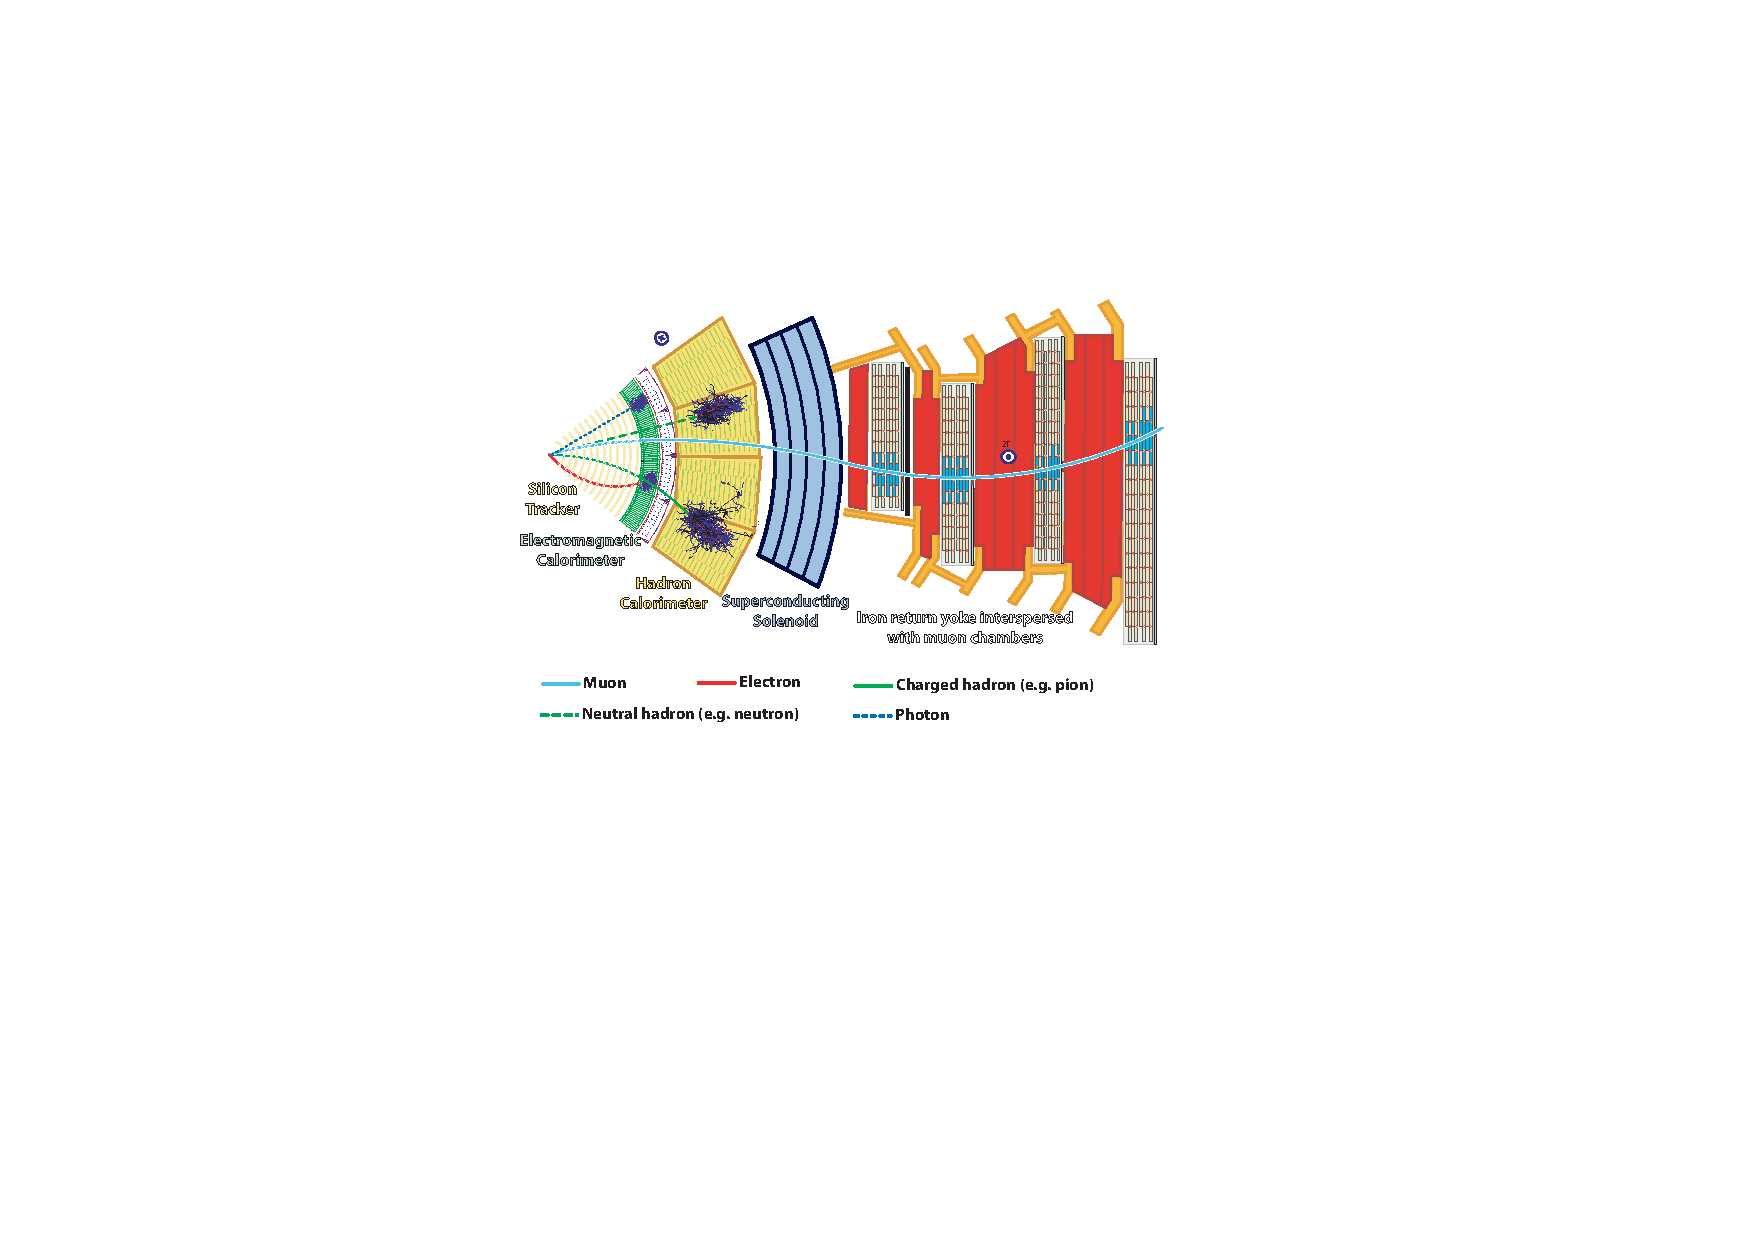
\includegraphics[width=0.5\textwidth]{slice}
  \caption{The path of different particles through a cross section of the CMS detector.}
  \label{reco:crosssec}
\end{figure}

\section{Electrons}
\todo[inline]{Why are electrons important phsyics objects}
\todo[inline]{Describe path that electrons make through the detector.}

\subsection{Triggering}

\subsection{Reconstruction}
Electrons are reconstructed in CMS using information from the pixel detector,
silicon strip tracker and the ECAL.

\subsubsection{Electron Clustering}
As electrons traverse the CMS tracker, the strong magnetic field causes the path
of the electrons to be curved in the azimuthal, $\phi$, direction. The electrons
radiate bremsstrahlung photons, so that when the electron energy reaches the
ECAL it is spread over a narrow strip in the phi direction.
\FigureRef{reco:brem} shows the fraction of energy radiated by bremsstrahlung for
electrons of energy $10$, $30$ and \unit{$50$}{\GeV}.

\begin{figure}[htb]
  \centering
  %\includegraphics[width=0.5\textwidth]{placeholder}
  \missingfigure{Fraction of energy radiated by bremsstrahlung from Electron
reconstruction in CMS}
  \caption{Fraction of electron energy, $E^{e}$, radiated away as bremsstrahlung
photons, $\sum E_{brem}^{\gamma}$ for electrons of energy }%$10$, $30$ and \unit{$50$}{\GeV}. From \cite{}.}
  \label{reco:brem}
\end{figure}

To measure the electron energy, including the bremsstrahlung photons, the
seperated deposits of energy need to be collected, using super-clustering
algorithms. 

In the barrel a ``hybrid'' algorithm is used. The hybrid algorithm proceeds by
identifying several hot crystals, with energies above a certain threshold, that
will act as seeds. The algorithm then forms $1\times3$ or $1\times5$ crystal
``dominos'', centered on the seed crystal, depending on the energy within the
domino. The dominos are then collected together in the $\phi$ direction, up to
an extension of \unit{0.3}{\rad}, to form clusters of clusters. This is
demonstrated in \FigureRef{fig:hybrid}.

\begin{figure}[htb]
  \centering
  %\includegraphics[width=0.5\textwidth]{placeholder}
  \missingfigure{hybrid clustering algorithm}
  \caption{Demonstration of the clustering of dominos in the hybrid algorithm.}
  \label{reco:hybrid}
\end{figure}

A ``multi5x5'' algorithm is used in the ECAL endcaps. Energy is collected in
$5\times5$ matrices, which are then collected together if their position lies on
a narrow $\phi$ road to form superclusters.

\subsubsection{Electron Seeding}
The superclusters are then used to select seeds for the track reconstruction.
Starting with a supercluster that passes a \pt and a hadronic veto, the
trajectory of the electron is propogated back through the magnetic field and
matched to the trajectory seeds, pairs or triplets of hits in the inner tracker.
If the trajectory seeds fall within a window of the supercluster path under
either charge hypothesis, they are selected and used to seed the track
reconstruction.
The ECAL driven seeding is comlemented by a tracker driven seeding algorithm.
This starts with high purity tracks and extrapolating them outwards to the ECAL.
This is effective for lower \pt electrons.

Seeds from both of the algorithms are collected and merged in to a single
collection, which is then used to seed the electron track reconstruction.

\subsubsection{Electron Track Reconstruction}
\todo[inline]{Rewrite this section}
The track reconstruction is based on a combinatorial Kalman filter,\todo{find a
citation for this} with the electron energy losses described using Bethe Heitler
modelling.

The track reconstruction starts with a seed, from which a tree of possible track
candidates is built from. 

%track reconstruction paper
Throughout the track reconstruction, tracks candidates are described by a state
vector containing information on the momentum, direction and position of the
track.

The Kalman filter is a
two step process. In the propogation step, track states are extrapolated to
the next layer of the detector, while taking in to account for energy losses due
to bremsstrahlung and coulomb scattering. 
In the update step, the extrapolated track state is 
combined with what is observed in that layer and the track is updated. 

The collected hits are passed to the GSF for a final fitting and estimation of
the track parameters. The GSF algorithm is similar to the Kalman filter but
energy losses are now described by a weighted sum of Gaussian distributions.
% corrections

\subsection{Electron Identification}
Electron identifiaction is based on a limited number of variables.
\todo{backgrounds to prompt electrons}

\subsubsection{Shape variable }

$\sigma_{\eta\eta}$ is the width of the electron shower in the $\eta direction$,
\begin{equation}
\sigma_{\eta\eta} = 
\sum_{\text{crystals}} \left(\eta_{i} - \eta{s}\right)^{2}
\frac{E_{i}}{E_{\text{seed cluster}}}.
\end{equation}

\subsubsection{Hadronic Energy}
Ratio of the energy deposited in the HCAL tower behind the electromagnetic seed
cluster to the energy of that seed cluster.

\subsubsection{Angular Separation of Track and Super Cluster}
$\Delta\phi$ and $\Delta\eta$ represent the angular separation between the
trajectory of the reconstucted GSF track, extrapolated to the ECAL, and the ECAL supercluster in the $\phi$
and $\eta$ direction respectivly.
\begin{align}
|\Delta\eta| &\equiv |\eta_{\text{SC}} - \eta_{track}|\\
|\Delta\phi| &\equiv |\phi_{\text{SC}} - \phi_{track}|
\end{align}

\subsubsection{Isolation}
For the calorimeter quantities

\subsubsection{Conversion Rejection}
Three further variables are included to reject electrons that are produced from
photon conversions. The missing hits is simply the number of layers in the inner
tracker where an expected hit from the track reconstruction is not detected by
the detector.
\todo{coversion partner tracks and dist and cot}
Coversion partner tracks are track candidates that are with in a cone of $\Delta
R < 0.3$ around the electron candidate track, and have an opposite charge. The
following two variables are used to detect \todo{what?} conversions.

\begin{equation}
\Delta \cot \theta \equiv \cot(\theta_{\text{KF}}) - \cot(\theta_{\text{GSF}})
\end{equation}
where $\theta_{KF}$ and $\theta_{GSF}$ are the polar angle of the conversion
partner track and the GSF track of the electron respectivly.

The variable, dist, is the distance between the two tracks where they are
parralel. \FigureRef{fig:dist} describes dist.

\begin{figure}[htb]
  \centering
  \missingfigure{Explanation of dist}
  %\includegraphics[width=0.5\textwidth]{placeholder}
  \caption{Dist is the distance between}
  \label{fig:dist}
\end{figure}

\subsubsection{Electron Identification Working Points}

Several sets of cuts have been produced for CMS analyses with different
efficiencies in mind. The cut values are sumarised in \TableRef{tab:electronwp}.
\todo{table of electron working points}

\subsection{Charge Identification}
The charge of an electron can be identified by studying how the electron trajectory
is bent in the magnetic field as the electron passes through the tracker. This
can be made difficult by conversion of bremsstrahlung photons when they are
radiated early. 

Within CMS, three methods of charge identifaction have been developed based on
the GSF track charge, the general track charge and the supercluster charge. The
GSF track charge is simply the sign of the curvature of the GSF fit of the
electron track. The general track charge is found by matching the GSF track with
general Kalman filter track by asking for shared hits in the pixel tracker. 
The super cluster charge is obtained by finding the sign of the phi difference
between the supercluster position and the first hit of the electron track.

At the \PZ peak, a charge mis-identification rate of \unit{3}{\%} is expected,
when using the electron trajectory from the GSF fit.  A sample with improved
charge identifaction can be obtained by using a majority method, that combines
the three measurements and assigns the sign from the 2 estimates out of three
that are in agreemenet, or by requiring that all three methods for assigning
charge are in agreement and discarding the event otherwise.

\section{Missing Energy}
\todo[inline]{Describe how MET is measured in CMS} 

\subsection{Particle Flow at CMS}
\todo[inline]{Tie particle flow in with rest of chapter.} 

New physics will manifest itself in CMS through signatures involving standard
model particles. Important signatures for many new phenomena include high \Pt\
jets, missing transverse energy (\met), jets containing \Pbottom quarks and
hadronically decaying tau leptons. To study these signatures it is important to
reconstruct and identify all particles in events as accurately as possible. The
particle-flow event reconstruction attempts to reconstruct and identify all
stable particles in an event by combining information from all CMS
sub-detectors. The particle reconstruction and identification starts with
collecting information from each subdetector to form elements such as tracks
and energy clusters in the calorimeters. These basic 'elements' are then
combined to form blocks which are then interpreted in terms of particles by the
particle flow algorithm. A list of individual particles is then returned from
the algorithm which can be used to study the event in greater detail by,
amongst other things, building jets, tagging b quarks and calculating missing
transverse energy.\cite{PF}

The first step of the particle-flow reconstruction algorithm is to collect the
fundamental elements. The elements consist of charged particles tracks from the
tracker, clusters of energy deposition in the calorimeters and muon tracks.
These elements need to be identified with a high efficiency and low fake rate
since the particle reconstruction depends on these basic elements and
misidentified elements could lead to missing or double counted
particles.\cite{PF}

As a particle traverses the detector it may interact with many CMS subdetectors
creating several particle-flow elements. A link algorithm is used to connect
the elements together to form blocks that typically contain 1, 2 or 3 elements.
The algorithm returns a distance between the elements as a measure of the
quality of the link. The final step of the particle flow algorithm is to
reconstruct and identify particles from each block of linked elements.\cite{PF}

Once the event has been fully reconstructed with the particle flow technique
the missing transverse energy (\met) in the event can be easily computed by
summing up the transverse momentum of all the reconstructed particles.\cite{PF}


  \chapter[Measurement of the Electron Charge Asymmetry]{Measurement of the Electron Charge Asymmetry with \unit{36}{\invpb} }
\label{chap:analysis}

In this chapter the measurement of the electron charge asymmetry is presented.
The analysis is performed on the full 2010 dataset, which corresponds to a
luminosity of \unit{36.1}{\invpb} at $\sqrtS = \unit{7}{\TeV}$
\cite{asym36,baisini2010electron}.

The results are presented in 6 bins of absolute value of pseudorapidity with a
fixed width of 0.4. To avoid the gap between the ECAL barrel and the ECAL endcap the
region $1.4<|\eta|<1.6$ is excluded.

\section{Event Selection}

The event selection is performed on single electron datasets formed of events
that are selected using various single photon and single electron triggers. From
these datasets, electrons are selected that pass a limited number of cuts.
Events that contain only a single electron are then selected for the analysis.

\subsection{Trigger}
\label{sec:trigger1}

Several high-level triggers (HLT) were used to select the events due to the
increasing luminosity during the {LHC} 2010 run.  In the initial runs, events
were selected using only a single photon trigger.  As the instantaneous
luminosity was increased and these triggers became prescaled, it was necessary
to use electron triggers to select events.  As the luminosity increased even
further, it was necessary to use electron triggers that included cuts on certain
electron ID variables.

In the following analysis, a control region is obtained by inverting the
selection on the $\Delta\phi$ and $\Delta\eta$ variables (see
\SectionRef{sec:eid}).
To ensure that this inverted selection is effective and will actually
select events, it is necessary to avoid using triggers that apply a selection on
these variables.

The triggers used to select the events are summarised in \TableRef{tab:triggers}
where ``HLT\_Ele$X$'' indicates a high-level trigger selection requiring an
electron with  $\Pt > \unit{X}{\GeV}$.  ``Photon'' in the name indicates that
the selection was applied to ECAL superclusters rather than a reconstructed
electron.  ``SW'' stands for small window, where window refers to the electron
pixel-matching window.  ``Cleaned'' indicates that spikes in the {ECAL} have
been removed.  

``CaloEleId'' and ``TighterCaloIdIso'' represent increasingly tighter selection
based on the shower shape ID and isolation variables from only the {ECAL},
and not the $\Delta\phi$ or $\Delta\eta$ variables.  


``TightEleId'' indicates a tight selection based on all ID variables. 
This nullifies the inverted cuts used for the control region but
it was the only trigger available for these runs without a prescale applied.
To compensate for the missing events in the control region, a looser prescaled
trigger was also applied in these runs.

\begin{table}[htbp]
  \centering
  \begin{tabular}{ l l }
    \toprule
    Run Ranges & Trigger String\\
    \midrule
    132440-137028 & \verb=HLT_Photon10_L1R= \\
    138564-140401 & \verb=HLT_Photon15_Cleaned_L1R= \\
    141956-144114 & \verb=HLT_Ele15_SW_CaloEleId_L1R= \\
    146428-147116 & \verb=HLT_Ele17_SW_CaloEleId_L1R= \\
    147196-148102 & \verb=HLT_Ele17_SW_TightEleId_L1R= \\
                  & \verb=HLT_Ele17_SW_L1R (prescaled)= \\ 
    148822-149063 & \verb=HLT_Ele22_SW_TighterCaloIdIso1_L1R_v1= \\
    149181-149442 & \verb=HLT_Ele22_SW_TighterCaloIdIso1_L1R_v2= \\
    \bottomrule
  \end{tabular}
  \caption{The triggers used to select the data used in this analysis.}
  \label{tab:triggers}
\end{table}

\subsection{Electron Selection}
The available high-level triggers place a lower limit on the electron \pT
threshold.
To avoid a changing HLT efficiency caused by the trigger-turn-on efficiency
curve the electron \PT is required to be
greater than \unit{25}{\GeV} in the analysis. 
The results are presented with an electron \pT cut of 25, 30
and \unit{35}{\GeV}. 

Electron candidates are identified using a cut-based approach on a limited
number of variables \cite{daskalakis2009data}.  The cut values used correspond
to the $80\%$ working point from \TableRef{tab:electronwp}, and are summarised
again in \TableRef{tab:electronselection}. The $80\%$ working point was chosen
as a compromise between ensuring high-enough statistical accuracy while maintaining
a high-enough purity of the sample.

\begin{table}[htbp]
  \begin{center}
    \leavevmode
    \begin{tabular}{lll} 
    \toprule
     Selection Variable & \multicolumn{2}{c}{Cut Value}\\
                        & Barrel & Endcap\\
\midrule 
  \multicolumn{3}{l}{\emph{ID Cuts}}\\
   H/E & 0.04 & 0.025 \\
  $\Delta\phi$ & 0.06 & 0.03 \\
  $\Delta\eta$ & 0.004 & 0.007  \\
  $\sigma_{\eta\eta}$ & 0.01 & 0.03 \\
  \midrule \multicolumn{3}{l}{\emph{Isolation Cuts}}\\
  $ISO_{trk} / E_T $  & 0.09 & 0.04 \\ 
  $ISO_{ecal}/ E_T$  & 0.07 & 0.05 \\
  $ISO_{hcal}/ E_T$  & 0.10 & 0.025 \\ 
  \midrule
   \multicolumn{3}{l}{\emph{Conversion Rejection Cuts}}\\
    Missing Hits  & \multicolumn{2}{c}{$\leq 0$}\\
    Dist (cm) $||$ Dcot   & \multicolumn{2}{c}{$>0.02$}\\
  \bottomrule 
  \end{tabular} 
  \caption[The electron selection variables and corresponding cut values.]
{\label{tab:electronselection}The electron selection variables and corresponding
cut values \cite{simplecutbasedeleid}.} 
  \end{center} 
\end{table}

Incorrectly assigning the charge of an electron will lead to a dilution of the
measured charge asymmetry.  An additional requirement is applied to the charge
of the reconstructed electron to reject events where the true charge is
difficult to determine.  The methods for assigning a charge to an electron are
described in \SectionRef{sec:charge}. The methods are based on the GSF electron
charge, the general track charge and the supercluster charge.
Electron candidates are only selected if all of the three methods agree on the
charge assignment.

The incorrect charge assignment rate can be measured at the Z peak by comparing
the same sign \HepProcess{\PZ\to\Pepm\Pepm} yield to the opposite sign
\HepProcess{\PZ\to\Pelectron\APelectron} yield. \FigureRef{fig:zpeak} show these
Z yields using only the {GSF} track charge (red) and also requiring a unanimous
assignment of charge from all three methods (blue). 

The incorrect charge assignment rate from the GSF track charge alone is about
$3\%$.  By requiring that all three methods for assigning the charge agree, and
vetoing events otherwise, the incorrect assignment rate can be reduced by a
factor of 8 with only a $5\%$ loss in efficiency \cite{baisini2010electron}.

\begin{figure}[htbp]
  \centering
  \begin{subfigure}{\textwidth}
    \centering
    \includegraphics[width=0.75\textwidth]{zpeak_os}
    \caption{Opposite sign \PZ peak.}
    \label{fig:zpeak_os}
  \end{subfigure}
  \begin{subfigure}{\textwidth}
    \centering
    \includegraphics[width=0.75\textwidth]{zpeak_ss}
    \caption{Same sign \PZ peak.}
    \label{fig:zpeak_ss}
  \end{subfigure}
  \caption[$Z\rightarrow ee$ peak.]
{ $Z\rightarrow ee$ peak. One electron is required to be in the
barrel to pass the electron selection and to have a fraction of energy loss by
radiation less than 0.3; the second electron is required only to pass the
electron selection \cite{baisini2010electron}.}\label{fig:zpeak} 
\end{figure}

\subsection{Event Selection}
An event is selected if it contains a single electron that passes all the
electron selection requirements.  To remove Drell-Yan events, an event is vetoed
if it contains a second electron passing a loose selection with $\PT >
\unit{15}{\GeV}$.  Events are also vetoed if they contain an isolated muon with
$\PT > \unit{15}{\GeV}$.

The expected composition of the selected events is measured from the MC
simulation samples, With a \pT cut of \unit{25}{\GeV} it is expected that $65\%$
of selected events are signal events, and of the remaining $35\%$ background
events, the majority are from {QCD} backgrounds with a small number from
{electroweak} processes, which are mostly Drell-Yan (DY) events. 

%\begin{table}[htbp]
%\begin{center}
%\begin{tabular}{llrrr}
    %\toprule
%& & $\PT>25$ \GeV & $\PT>30$ \GeV & $\PT>35$ \GeV  \\
%\midrule
%Signal & \HepProcess{\PW\to\Pe\Pnu} & $65.1\%$&$63.5\%$ &$60.2\%$ \\
%Electroweak & \HepProcess{\PZ\to\Ptau\Ptau} & $0.4\%$ &$0.3\%$  &$0.2\%$ \\
    %& \HepProcess{\PZ\to\Pe\Pe}     & $4.1\%$ &$3.5\%$  &$3.0\%$\\
    %& \HepProcess{\PW\to\Ptau\Pnu}  & $1.9\%$ &$1.1\%$  &$0.6\%$\\
    %& \HepProcess{\Ptop\APtop}      & $0.3\%$ &$0.3\%$  &$0.3\%$\\
    %& Total                         & $6.7\%$ &$5.2\%$  &$4.1\%$\\
%QCD & Total                         & $28.2\%$&$31.3\%$ &$35.7\%$\\
    %\bottomrule
%\end{tabular}
%\caption[Composition of selected events.]{Composition of selected events for lepton momentum cut of
%$\PT>\unit{25}{\GeV}$, $\PT>\unit{30}{\GeV}$ and $\PT>\unit{35}{\GeV}$ from
%{MC} simulation\cite{baisini2010electron}.}
%\label{tab:selectedcomp}
%\end{center}
%\end{table}

The particle flow \ETm distribution for the events that pass the event
selection, with an electron cut of $\PT > \unit{25}{\GeV}$ and $|\eta| < 2.4$ is
shown in \FigureRef{fig:pfmet_dist_36}. There are two obvious peaks in the
distribution. The peak at $\ETm \approx \unit{40}{\GeV}$ is the
\HepProcess{\PW\to\Pe\Pnue} signal region. This region also contains
\HepProcess{\PW\to\Ptau\Pnut} backgrounds. The peak at
$\ETm\approx \unit{10}{\GeV}$ is the background region that contains the {QCD}
and {DY} background events.

\begin{figure}[htbp]
  \begin{center}
    \includegraphics*[width=0.8\textwidth]{pfmet_dist}
    \caption[Particle Flow \ETm distribution for selected events.]{Particle Flow
\ETm distribution for selected events with an electron cut of $\PT >
\unit{25}{\GeV}$ and $|\eta| < 2.4$\cite{baisini2010electron}.\label{fig:pfmet_dist_36}}
  \end{center}
\end{figure}

The number of selected events that pass the
event selection are shown in \TableRef{tab:selectedevents}. To obtain a
measurement of the asymmetry from the selected events it is necessary to extract
the signal yield from each pseudorapidity/charge bin.

\begin{table}[htbp]
\begin{center}
%\begin{sideways}
\begin{tabular}{lcrrr}
    \toprule
  $|\eta|$ range & Charge & \multicolumn{3}{c}{Selected Events}\\
                 &        & $\PT>25$ \GeV & $\PT>30$ \GeV & $\PT>35$ \GeV\\
\midrule
$0.0<| \eta |<0.4$ &$+$& 18956&14232&9885\\
                   &$-$& 15060&11505&8105\\
$0.4<| \eta |<0.8$ &$+$& 20118&14966&10345\\
                   &$-$& 15736&11780&8307\\
$0.8<| \eta |<1.2$ &$+$& 20681&15091&10184\\
                   &$-$& 16167&11735&8112\\
$1.2<| \eta |<1.4$ &$+$& 10646&7606&5161\\
                   &$-$& 8226&5871&4067\\
$1.6<| \eta |<2.0$ &$+$& 16426&11877&7814\\
                   &$-$& 11678&8578&5886\\
$2.0<| \eta |<2.4$ &$+$& 18885&13239&8726\\
                   &$-$& 13226&9227&6184\\
    \bottomrule
\end{tabular}
%\end{sideways}
\end{center}
\caption[Number of events passing the event selection.]{Number of events passing
the event selection for lepton momentum cuts of $\PT> \unit{25}{\GeV}$, $\PT>
\unit{30}{\GeV}$ and $\PT>\unit{35}{\GeV}$ \cite{baisini2010electron}.}
    \label{tab:selectedevents}
\end{table}


\section{Signal Yield Extraction Method}
The number of signal and background events in each bin is extracted using a
maximum likelihood fit to the \ETm distribution using two fixed templates shapes
\cite{adam2007towards}, similar to the method used in the measurement of the \PW
cross section \cite{alcaraz2010updated}.
The first template is the sum of the \Wenu signal and the {electroweak}
background shapes, and the second template is the sum of the {QCD} plus \gjet
processes.

\subsection{{QCD} \ETm Shape}
The \ETm distribution for the {QCD} and \gjet background is obtained from a control.
The control sample is selected by requiring that the electrons pass the
isolation and $H/E$ cuts but fail the $\Delta\phi$ and $\Delta\eta$ cuts as
shown in \TableRef{tab:antisel}.

\begin{figure}[htbp]
  \centering
  \begin{subfigure}{0.4\textwidth}
    \centering
    \includegraphics*[trim = 0mm 0mm 15mm 0mm, clip, width=\textwidth, angle=90]{MetCompare_anti_eta1.pdf}
    \caption{$0.0<| \eta |<0.4$}
    \label{fig:qcd_met_eta1}
  \end{subfigure}
  \begin{subfigure}{0.4\textwidth}
    \centering
    \includegraphics*[trim = 0mm 0mm 15mm 0mm, clip, width=\textwidth, angle=90]{MetCompare_anti_eta2.pdf}
    \caption{$0.4<| \eta |<0.8$}
    \label{fig:qcd_met_eta2}
  \end{subfigure}
  \begin{subfigure}{0.4\textwidth}
    \centering
    \includegraphics*[trim = 0mm 0mm 15mm 0mm, clip, width=\textwidth, angle=90]{MetCompare_anti_eta3.pdf}
    \caption{$0.8<| \eta |<1.2$}
    \label{fig:qcd_met_eta3}
  \end{subfigure}
  \begin{subfigure}{0.4\textwidth}
    \centering
    \includegraphics*[trim = 0mm 0mm 15mm 0mm, clip, width=\textwidth, angle=90]{MetCompare_anti_eta4.pdf}
    \caption{$1.2<| \eta |<1.4$}
    \label{fig:qcd_met_eta4}
  \end{subfigure}
  \begin{subfigure}{0.4\textwidth}
    \centering
    \includegraphics*[trim = 0mm 0mm 15mm 0mm, clip, width=\textwidth, angle=90]{MetCompare_anti_eta5.pdf}
    \caption{$1.6<| \eta |<2.0$}
    \label{fig:qcd_met_eta5}
  \end{subfigure}
  \begin{subfigure}{0.4\textwidth}
    \centering
    \includegraphics*[trim = 0mm 0mm 15mm 0mm, clip, width=\textwidth, angle=90]{MetCompare_anti_eta6.pdf}
    \caption{$2.0<| \eta |<2.4$}
    \label{fig:qcd_met_eta6}
  \end{subfigure}
  \caption[The \ETm distribution in anti-selected {MC}
simulated events and selected {QCD} and \gjet background MC simulated events.]
{The \ETm distribution in data and background anti-selected {MC} simulated
events and selected {QCD} and \gjet background MC simulated events in each
pseudorapidity bin\cite{baisini2010electron}.}
  \label{tab:antiselclosure}
\end{figure}

\begin{table}[htbp]
  \begin{center}
    \leavevmode
    \begin{tabular}{lcc} 
    \toprule
      Selection Variable & \multicolumn{2}{c}{Cut Value}\\
                         & Barrel & Endcap\\
    \midrule
        H/E & 0.04 & 0.025 \\
        $\Delta\phi$ & $>0.06$  & $>0.04$ \\
        $\Delta\eta$ & $>0.007$ & $>0.009$\\
        $ISO_{trk} / E_T $ & 0.09 & 0.04 \\
        $ISO_{ecal}/ E_T$  & 0.07 & 0.05 \\
        $ISO_{hcal}/ E_T$  & 0.10 & 0.025\\ 
    \bottomrule
    \end{tabular}
    \caption[Electron anti-selection variables and corresponding cut values.]
{\label{tab:antisel} Electron anti-selection variables and corresponding cut
values. The $\Delta\phi$ and $\Delta\eta$ cuts are
inverted\cite{baisini2010electron}.}
  \end{center}
\end{table}

To validate the anti-selection used, {QCD} Monte Carlo (MC) simulation samples are used. The
distribution of {QCD} MC events passing the event selection is compared to the
anti-selected MC events. This is shown for each pseudorapidity bin in
\FigureRef{tab:antiselclosure}. The agreement is seen to be good with little
signal contamination in the control region.

\subsection{Signal \ETm Shape from Boson Recoil}
\label{sec:recoil}
The \ETm in signal events arises from the unmeasured neutrino in the event. 
The signal \ETm shape is derived from MC simulations with an event-by-event
correction applied to account for differences in the \ETm scale and resolution
between data and MC.
The correction is based on the hadronic recoil distribution measured in data.
The recoil response and resolution in \HepProcess{\PZ\to\Plepton\Plepton} data
events is measured as a function of the \pT of the boson. This is combined with
information from the \PW and \PZ MC simulation to derive a correction to
the simulated \ETm as a function of \PW boson's \pT
\cite{bauer2010modeling,alcaraz2010updated}.

The transverse recoil vector, $\vec{U}$, is calculated from the reconstructed
transverse missing energy, $\vec{E}_{\mathrm{T}}^{\mathrm{miss}}$, and the
electron \pT vectors,
\begin{align}
\vec{U} &= - \vec{E}_{\mathrm{T}}^{\mathrm{miss}} 
      - \vec{p}^{\ \mathrm{e}}_{\mathrm{T}}\\
\vec{U} &= - \vec{E}_{\mathrm{T}}^{\mathrm{miss}} 
      - \sum_i \vec{p}^{\ \mathrm{e}_i}_{\mathrm{T}}
\end{align}
for \PW events and \PZ events respectively. $\vec{U}$ is split into components
that are parallel ($U_1$) and perpendicular ($U_2$) to the true boson \pT
direction. 
In \PZ data events the true boson \pT is not known and is reconstructed from the
\pT of the two electrons.

The hadronic activity that balances the \pT of the boson will lie mostly in the
$U_1$ direction whereas $U_2$ will be mostly formed from other sources.
\FigureRef{fig:recoil} shows the decomposition of $\vec{U}$ into $U_1$ and
$U_2$ in W events \cite{bauer2010modeling}.
\begin{figure}
  \begin{center}
    \includegraphics*[width=0.85\textwidth]{recoil}
    \caption[The decomposition of $\vec{U}$ for \PW events.] {The decomposition
of $\vec{U}$ for \PW events. Modified from \cite{bauer2010modeling}.}
    \label{fig:recoil}
  \end{center}
\end{figure}

$U_1$ and $U_2$ are measured in \PZ data, \PZ MC simulation and \PW MC
simulation and are then binned in units of the boson \pT.  In each $p_T^{Z}$ bin
the $U_1$ and $U_2$ distributions are fitted with a Gaussian.  A linear function,
$f_i(p_T^Z)$, is fit to the distribution of the Gaussian means to produce a
response curve for both data and MC.  A second order polynomial,
$\sigma_i(p_T^Z)$, is then fit to the distribution of the Gaussian widths to
produce a resolution curve for both data and MC\cite{bauer2010modeling}.

The fitting procedure results in two response functions, $f_i(p_T)$, and two
resolution functions, $\sigma_i(p_T)$, for \PZ data, \PZ MC events and
the \PW MC events. The functions are then used to define a set of \PW
MC corrected functions, 

\begin{align}
f^{corr}_i (p^{W}_T)      
  &= \frac{ f^{Z\ data}_i (p^{Z}_T) }
          { f^{Z\ MC}_i (p^{Z}_T) }
          f^{W\ MC}_i (p^{W}_T) \\
\sigma^{corr}_i (p^{W}_T) 
  &= \frac{ \sigma^{Z\ data}_i (p^{Z}_T) }
          { \sigma^{Z\ MC}_i (p^{Z}_T) }
          \sigma^{W\ MC}_i (p^{W}_T) 
\end{align}

The corrected recoil response and resolution curves are then used to correct the
\PW MC \ETm. For each \PW MC event, the generator level \pT of the boson is
found, and the values for the response, $f^{corr}_i (p^{W}_T)$, and
resolution curves, $\sigma^{corr}_i (p^{W}_T) $, are looked up. A Gaussian is
defined with these values and then sampled to determine the new recoil
components $U_i$,
\begin{equation}
U_i \sim Gaus(f^{corr}_i (p^{W}_T), \sigma^{corr}_i (p^{W}_T) ).
\end{equation}
The components are then combined to form the new corrected recoil vector
$\vec{U^{\prime}}$ which is then combined with the electron vector to
form the corrected \ETm\cite{bauer2010modeling}.

The modelling of the \HepProcess{\PW\to\Plepton\Pnu} \ETm with boson recoil is
described in detail in reference \cite{bauer2010modeling}. 
Ntuples containing \HepProcess{\PW\to\Pelectron\Pnu} simulation with the recoil corrected \ETm were
provided from reference \cite{alcaraz2010updated}.

\subsection{{Electroweak} \ETm Shape}
The electroweak background processes that can produce a single isolated
electron which are considered in this analysis are:
\begin{itemize}
\item \HepProcess{\PZ\to\Pelectron\APelectron}, where one of the electrons falls
outside the geometric acceptance or is not detected,
\item \HepProcess{\PZ\to\Ptauon\APtauon}, where one of the taus decays
to an electron and the other decays hadronically, or semi-leptonically and the lepton
is not detected,
\item \HepProcess{\PW\to\Ptau\Pnu}, where the tau decays to an electron,
\item \HepProcess{\Ptop\APtop}, where an electron is produced.
\end{itemize}

The \ETm distributions for the {electroweak} background were obtained from
PYTHIA\cite{pythia} MC simulations for each pseudorapidity/charge bin.  The MC samples used
are summarised in \TableRef{tab:samples36}.  The scale of the {electroweak}
shape is fixed to the signal \ETm shape by the ratio obtained from MC samples.

\subsection{Fit Results}

The results of the extended maximum likelihood fits to each pseudorapidity/charge
bin are shown the appendix in \FigureRef{fig:fit1} and \FigureRef{fig:fit2} and
the $\chi^2$ of each fit is included in \TableRef{tab:chi2}.
%The signal yield in each bin is summarised in \TableRef{tab:sigyield} and 
%The ratio between the fits and the data for each of the 
%bins are shown in \FigureRef{fig:fit1ratio} and \FigureRef{fig:fit2ratio}.


%\begin{table}[htbp]
%\begin{center}
%\begin{tabular}{lcrrr}
    %\toprule
%$|\eta|$ range & Charge & \multicolumn{3}{c}{Signal Yield}\\
               %&        & $\PT>25$ \GeV & $\PT>30$ \GeV & $\PT>35$ \GeV  \\
%\midrule
%$0.0<| \eta |<0.4$ &$+$& 12866&  9992&  6955\\
                   %&$-$&  9432&  7646&  5476\\
%$0.4<| \eta |<0.8$ &$+$& 13413&  9596&  6898\\
                   %&$-$&  9627&  7128&  5376\\
%$0.8<| \eta |<1.2$ &$+$& 12684&  9161&  5947\\
                   %&$-$&  9013&  6803&  4560\\
%$1.2<| \eta |<1.4$ &$+$&  6220&  4427&  2895\\
                   %&$-$&  4349&  3247&  2231\\
%$1.6<| \eta |<2.0$ &$+$&  9033&  6285&  4079\\
                   %&$-$&  5850&  4270&  2905\\
%$2.0<| \eta |<2.4$ &$+$&  9104&  6965&  4259\\
                   %&$-$&  5420&  4335&  2775\\
    %\bottomrule
%\end{tabular}
%\end{center}
%\caption[The signal yield in each pseudorapidity bin after the fitting
%procedure.]{The signal yield in each pseudorapidity bin after the fitting
%procedure\cite{baisini2010electron}.}
    %\label{tab:sigyield}
%\end{table}

\begin{table}[htbp]
\begin{center}
\begin{tabular}{lcr}
    \toprule
$|\eta|$ range &Charge & $\chi^2$/ndof of Fit\\
\midrule
$0.0<| \eta |<0.4$ &$+$&  0.86\\
                   &$-$&  0.84\\
$0.4<| \eta |<0.8$ &$+$&  0.99\\
                   &$-$&  1.36\\
$0.8<| \eta |<1.2$ &$+$&  1.05\\
                   &$-$&  1.13\\
$1.2<| \eta |<1.4$ &$+$&  0.97\\
                   &$-$&  1.30\\
$1.6<| \eta |<2.0$ &$+$&  1.38\\
                   &$-$&  1.61\\
$2.0<| \eta |<2.4$ &$+$&  1.44\\
                   &$-$&  1.11\\
    \bottomrule
\end{tabular}
\caption[$\chi^2$/ndof of the fits in each pseudorapidity
bin.]{\label{tab:chi2}$\chi^2$/ndof of the fits in each pseudorapidity
bin\cite{baisini2010electron}.}
\end{center}
\end{table}


\subsection{Validation of Signal Extraction Method on Simulation}

The signal yield extraction procedure was validated using pseudo-data
experiments. 1000 pseudo-data experiments were generated with the number of
events expected in \unit{36.1}{\invpb} of data. The signal yields are extracted
in each experiment and the asymmetry is calculated. The distribution of
asymmetries is then fitted with a Gaussian.
The measured asymmetry for the 1000 pseudo-data experiments distribution for each
pseudorapidity bin is shown in \FigureRef{fig:toyasym}.

The width of the Gaussian is the statistical uncertainty on the measurement.
The statistical uncertainty can also be estimated from the following formula
\begin{equation}
  \label{tab:statuncert}
\sigma_\mathcal{A} = 
\frac{ 
  2 \times \sqrt{ \left( N^+ \sigma_{N^-} \right)^2 + \left( N^- \sigma_{N^+} \right)^2 } 
}
{ 
  \left( N^{+} + N^{-} \right)^2 
} .
\end{equation}
where $\sigma_\mathcal{A}$ is the statistical uncertainty on the asymmetry
measurement in a given pseudorapidity bin, $N^{\pm}$ is the measured signal
yield in a given pseudorapidity/charge bin and $\sigma_{N^\pm}$ is the
statistical uncertainty on the measured signal yield in each bin.

The uncertainty from \EquationRef{tab:statuncert} evaluated with {MC} truth
values, and the uncertainty measured from pseudo-data experiments for an
integrated luminosity of \unit{36.1}{\invpb} are summarised in
\TableRef{tab:statuncertsum} , and are in good agreement.

\begin{table}[htbp]
  \begin{center}
    \begin{tabular}{lcc}
    \toprule
    $|\eta|$ range & $\sigma_{A}$ from \EquationRef{tab:statuncert}. & $\sigma_{A}$ from pseudo-data exp.\\ \midrule
    $0.0<|\eta|<0.4$ & 0.0064 & 0.0062\\
    $0.4<|\eta|<0.8$ & 0.0064 & 0.0064\\
    $0.8<|\eta|<1.2$ & 0.0065 & 0.0065\\
    $1.2<|\eta|<1.4$ & 0.0096 & 0.0104\\
    $1.6<|\eta|<2.0$ & 0.0076 & 0.0079\\
    $2.0<|\eta|<2.4$ & 0.0077 & 0.0077\\
    \bottomrule
    \end{tabular}
  \caption[Expected statistical error from {MC} simulation and pseudo-data
experiments]{Expected statistical error from {MC} simulation and pseudo-data
experiments as a function of pseudorapidity, for an integrated luminosity of
\unit{36}{\invpb}\cite{baisini2010electron}. }
  \label{tab:statuncertsum}
  \end{center}
\end{table}

The distributions of the asymmetry measurements in each pseudo-data experiment
are shown in \FigureRef{fig:toyasym}. The true MC value of the asymmetry is
shown with a vertical line, and the Gaussian fit is also shown.
The results show good agreement with the true value which implies an unbiased
measurement.

%The pull is defined as the difference between the asymmetry measured
%from pseudo-data experiments and the true MC value for the asymmetry divided by
%the statistical uncertainty. The pull on the asymmetry measurment is small.

%\begin{table}[htbp]
  %\begin{center}
    %\begin{tabular}{lcc}
    %\toprule
    %$|\eta|$ range & Pull \\
    %$0.0<|\eta|<0.4$ & $-0.07 $\\
    %$0.4<|\eta|<0.8$ & $-0.15 $\\
    %$0.8<|\eta|<1.2$ & $ 0.00 $\\
    %$1.2<|\eta|<1.4$ & $ 0.04 $\\
    %$1.6<|\eta|<2.0$ & $ 0.12 $\\
    %$2.0<|\eta|<2.4$ & $ 0.07 $\\
    %\bottomrule
    %\end{tabular}
  %\caption{Pulls on the asymmetry measurement \cite{baisini2010electron}. }
  %\label{tab:pulls}
  %\end{center}
%\end{table}

\begin{figure}[htbp]
  \begin{center}
    \includegraphics*[angle=90,width=0.95\textwidth]{toyasym.pdf}
    \caption[Measured asymmetry for 1000 pseudo-data experiments.]
{\label{fig:toyasym}Measured asymmetry for 1000 pseudo-data experiments. The
distribution of the measured asymmetry is fitted with a
Gaussian\cite{baisini2010electron}.}
  \end{center}
\end{figure}

%\begin{figure}[htbp]
  %\begin{center}
%\includegraphics*[angle=90,width=0.95\textwidth]{pullasyTot.pdf}
    %\caption{\label{fig:toyasym_pull}Pull on the asymmetry in 1000 pseudo-data experiments. The distribution of the pull is fitted with a Gaussian\cite{baisini2010electron}.}
  %\end{center}
%\end{figure}

\section{Corrections to the Measured Asymmetry}
\label{sec:corrections1}
After the signal extraction procedure the measured asymmetry is simply,
\begin{equation}
\mathcal{A}_{meas} = \frac{
\label{eq:meas}
  N_{meas}^{+} -
  N_{meas}^{-}
}
{
  N_{meas}^{+} +
  N_{meas}^{-}
},
\end{equation}
where $N_{meas}^{+}$ and $N_{meas}^{-}$ are number of positrons and
electrons extracted with the fitting procedure.
To compare with the theoretical value, the measured lepton asymmetry has to be
corrected for three detector effects,
\begin{itemize}
\item charge-dependent reconstruction efficiency,
\item incorrect charge assignment rate,
\item electron energy resolution.
\end{itemize}

If the reconstruction efficiency of electrons is different to that of positrons
then a bias will be introduced into the measured asymmetry, which will need to
be taken into account in the calculation of the asymmetry.  

The second experimental effect is due the incorrect charge assignment of electrons.
The incorrect charge assignment rates, $\omega^+$ and $\omega^-$, are the rate
at which electrons are incorrectly assigned a positive charge and identified as
positrons and the rate that positrons are identified as electrons, respectively.  The
incorrect assignment induces a dilution factor to the asymmetry as a function of
the electron pseudorapidity. 

The true asymmetry at the reconstruction level is defined as,
\begin{equation}
\label{eq:reco}
\mathcal{A}_{reco} = \frac{
  N_{reco}^{+} -
  N_{reco}^{-}
}
{
  N_{reco}^{+} +
  N_{reco}^{-}
},
\end{equation}
where $N_{reco}^{+}$ and $N_{reco}^{-}$ are the true number of positrons and
electrons with \pT greater than the threshold.  $N_{meas}^{+}$, $N_{meas}^{-}$
and $N_{reco}^{+}$, $N_{reco}^{-}$ are related by the efficiency of electrons
and positrons ($\epsilon^{-}$ and $\epsilon^{+}$) and the incorrect charge
assignment rates ($\omega^{+}$ and $\omega^{-}$),
\begin{align}
  \label{eq:poscor}
  N_{meas}^{+} 
  &= \epsilon^+ \left( ( 1 - \omega^- ) N_{reco}^{+} + \omega^+ N_{reco}^{-} \right)\\
  \label{eq:negcor}
  N_{meas}^{-} 
  &= \epsilon^- \left( ( 1 - \omega^+ ) N_{reco}^{-} + \omega^- N_{reco}^{+} \right).
\end{align}

The Equations (\ref{eq:poscor}) and (\ref{eq:negcor}) can then be inserted
into the definition of the measured asymmetry, \EquationRef{eq:meas}, to obtain,

\begin{equation}
\label{eq:meas1}
\mathcal{A}_{meas} = \frac{
  \epsilon^+ ( ( 1 - \omega^- ) N_{reco}^{+} + \omega^+ N_{reco}^{-} ) -
  \epsilon^- ( ( 1 - \omega^+ ) N_{reco}^{-} + \omega^- N_{reco}^{+} )
}
{
  \epsilon^+ ( ( 1 - \omega^- ) N_{reco}^{+} + \omega^+ N_{reco}^{-} ) +
  \epsilon^- ( ( 1 - \omega^+ ) N_{reco}^{-} + \omega^- N_{reco}^{+} )
} .
\end{equation}
The above can be simplified by first assuming that the rate at which
electrons are assigned a positive charge is the same as the rate at which positrons
are assigned a negative charge, \ie\cite{baisini2010electron} 
\begin{equation}
  \omega^{+} = \omega^{-} = \omega ,
\end{equation}
A further simplification is to introduce the relative detection efficiency, $R$,
which is defined as the ratio of electron efficiency to the positron efficiency,

\begin{equation}
 R = \epsilon^+/\epsilon^- ,
\end{equation}
which can be substituted into \EquationRef{eq:meas1},
\begin{align}
\mathcal{A}_{meas} 
&= \frac{
  N_{reco}^{+} (R - \omega(R+1)) -
  N_{reco}^{-} (1 - \omega(R+1))
}
{
  N_{reco}^{+} (R - \omega(R-1)) +
  N_{reco}^{-} (1 + \omega(R-1))
}\\
&= \frac{
  (1+\mathcal{A}_{reco}) (R - \omega(R+1)) -
  (1-\mathcal{A}_{reco}) (1 - \omega(R+1))
}
{
  (1+\mathcal{A}_{reco}) (R - \omega(R+1)) -
  (1-\mathcal{A}_{reco}) (1 + \omega(R-1))
}\\
&= \frac{
  \mathcal{A}_{reco} (R + 1)(1 - 2 \omega) + (R - 1)
}
{
  \mathcal{A}_{reco} (R - 1)(1 - 2 \omega) + (R - 1)
},
\end{align}
which can then be inverted to derive $\mathcal{A}_{reco}$ as a function of the
measured asymmetry ($\mathcal{A}_{meas}$), the relative efficiency ($R$) and the
incorrect charge assignment rate ($\omega$),
\begin{align}
\mathcal{A}_{reco}
&=\frac{1}{1-2\omega}
  \frac{
    \mathcal{A}_{meas} (R + 1) - (R-1)
  }
  {
    (R + 1) - \mathcal{A}_{meas} (R-1)
  }\\
&\approx \frac{1}{1-2\omega}
\left(
  \mathcal{A}_{meas} -
\frac{ (R - 1)(1 - \mathcal{A}_{meas}^{2}) } { 2 }
\right)
\end{align}

The measurements of the parameters $R$ and $\omega$, as well as the
uncertainties, are detailed in the following sections.

The electron energy resolution and energy scale can also introduce a systematic
bias on the asymmetry due to the effect of the transverse momentum cut applied
to the electrons. The largest source of the electron energy scale is the
radiation-induced change to the ECAL crystal transparency.  To correct for this
effect, energy scale and resolution corrections are derived using a \Zee mass
distribution. The results are presented in the following sections.

\subsection{Relative Efficiency}

If the reconstruction efficiency of electrons is different to that of
positrons then the measured asymmetry will be diluted and will need to be
corrected.

The efficiency for electrons and positrons is measured using the tag and probe
method \cite{adam2009tag} with a sample of \Zee events from the same datasets
used in the analysis.  The \Zee events offer a high purity source of unbiased
electrons with which to measure the efficiencies.

From the sample of \Zee events a ``tag'' electron is selected with strict
selection criteria. 
A ``probe'' electron is selected with the same electron selection described
earlier.
The invariant mass of the tag-probe pair is required to be
$\unit{60}{\GeV} < M_{ee} < \unit{120}{\GeV}$ to ensure a high purity sample.

Efficiencies can then be calculated by measuring the signal yield in events
with one tag electron and one probe passing the selection (tag \& pass) and
events where the probe electron fails the selection (tag \& fail).
The signal yield is extracted using a simultaneous maximum likelihood fit to
both the tag \& pass and the tag \& fail samples.

For this analysis the efficiencies are measured in two parts:

\begin{itemize}
    \item GSF tracking efficiency, $\epsilon_{GSF}$.
    \item Identification efficiency, including conversion rejection, unanimous
charge assignment and HLT request, $\epsilon_{ID}$.
\end{itemize}
The ratios $R_{GSF} = \nicefrac{\epsilon^{+}_{GSF}}{\epsilon^{-}_{GSF}}$ and
$R_{ID} = \nicefrac{\epsilon^{+}_{ID}}{\epsilon^{-}_{ID}}$ are found and the
overall efficiency ratio is given by $R = R_{GSF} R_{ID}$.
\TableRef{tab:tagprobe} shows the GSF tracking efficiency and identification 
efficiency as a function of the charge.

\begin{table}[htbp]
\begin{center}
\begin{tabular}{lcrrrr}
\toprule
$|\eta|$ range & Charge & $\epsilon_{GSF}$ &$\epsilon_{ID}$& R\\
\midrule
$0.0<| \eta |<1.4$ &$+$& $98.8\pm0.5$ &$84.1\pm0.8$ & $1.007\pm0.015$\\
                   &$-$& $98.4\pm0.5$ &$83.8\pm0.8$ & \\
$1.6<| \eta |<2.4$ &$+$& $98.3\pm0.7$ &$70.7\pm1.4$ & $0.99\pm0.03$\\
                   &$-$& $97.8\pm0.7$ &$71.5\pm1.4$ & \\
\midrule
$0.0<| \eta |<2.4$ &$+$& $98.5\pm0.4$ &$80.3\pm0.7$ & $1.007\pm0.014$\\
                   &$-$& $97.8\pm0.4$ &$80.3\pm0.7$ & \\
\bottomrule
\end{tabular}
\end{center}
\caption[GSF track reconstruction and electron identification efficiency as a
function of charge.]{GSF track reconstruction and
electron identification efficiency as a function of charge in the barrel and endcap
separately and the full inclusive range\cite{baisini2010electron}.}
\label{tab:tagprobe}
\end{table}

%\begin{table}[htbp]
%\begin{center}
%\begin{sideways}
%\begin{tabular}{cccccccc}
    %\toprule
%$|\eta|$  & \multicolumn{3}{c}{GSF tracking } & \multicolumn{3}{c}{ID } & $R$ \\
%region    & $\epsilon_{GSF}^+$ (\%) &$\epsilon_{GSF}^-$ (\%) & $R_{\epsilon_{GSF}}$ 
                                              %& $\epsilon_{ID}^+$ (\%) &$\epsilon_{ID}^-$ (\%) & $R_{\epsilon_{ID}}$ &  \\
%\midrule
%$\left[ 0.0,0.4 \right]$ & 95.7$\pm$1.1 & 97.5$\pm$1.0 & 0.982$\pm$0.015 & 71.2$\pm$1.5 & 68.4$\pm$1.5 & 1.04$\pm$0.03 &1.02$\pm$0.035  \\
%$\left[ 0.4,0.8 \right]$ & 98.8$\pm$ 1.0& 98.5$\pm$1.1 & 1.003$\pm$0.015 & 72.5$\pm$1.7 & 75.6$\pm$1.6 & 0.96$\pm$0.04 &0.96$\pm$ 0.04 \\
%$\left[ 0.8,1.2 \right]$ & 97.6$\pm$ 1.0& 98.4$\pm$1.0 & 0.992$\pm$0.015 & 77.4$\pm$1.5 & 74.4$\pm$1.7 & 1.04$\pm$0.04 &1.03$\pm$ 0.04 \\
%$\left[ 1.2,1.4 \right]$ & 96.2$\pm$ 1.5& 96.3$\pm$1.5 & 0.999$\pm$0.022 & 69.3$\pm$2.7 & 73.0$\pm$2.6 & 0.95$\pm$0.05 &0.95$\pm$0.05  \\
%$\left[ 1.6,2.0 \right]$ & 96.8$\pm$ 1.2& 96.9$\pm$1.0 & 0.999$\pm$0.015 & 61.9$\pm$2.0 & 63.6$\pm$2.0 & 0.97$\pm$0.05 &0.97$\pm$0.05  \\
%$\left[ 2.0,2.4 \right]$ & 96.4$\pm$ 1.1& 97.0$\pm$1.0 & 0.994$\pm$0.015 & 58.2$\pm$2.1 & 56.7$\pm$2.1 & 1.03$\pm$0.05 &1.02$\pm$0.05  \\
%\midrule
%$\left[ 0.0,1.4 \right]$ & 98.8$\pm$0.5 & 98.4 $\pm$0.5 & 1.004$\pm$0.007 & 84.1$\pm$0.8 & 83.8$\pm$0.8 & 1.003$\pm$0.014 & 1.007$\pm$ 0.015 \\
%$\left[ 1.6,2.4 \right]$ & 98.3$\pm$0.7 & 97.8 $\pm$0.7 & 1.005$\pm$0.010 & 70.7$\pm$1.4 & 71.5$\pm$1.4 & 0.99$\pm$0.03 &0.99$\pm$ 0.03 \\
%\midrule 
%$\left[ 0.0,2.4 \right]$ & 98.5$\pm$0.4 & 97.8$\pm$0.4 & 1.007$\pm$0.006 & 80.3$\pm$0.7 & 80.3$\pm$0.7 & 1.000$\pm$0.012 &1.007$\pm$0.014  \\
    %\bottomrule
%\end{tabular}
%\end{sideways}
%\end{center}
%\caption[GSF track reconstruction and electron identification efficiency as a
%function of charge in each pseudorapidity bin.]{GSF track reconstruction and
%electron identification efficiency as a function of charge in each
%pseudorapidity bin. The efficiencies are also shown for the barrel and endcap
%separately and the full inclusive range\cite{baisini2010electron}.}
%\label{tab:tagprobe}
%\end{table}


The main systematic errors on the efficiency measurements are the energy scale
and the signal shape used to extract the signal yield. Fortunately, these
errors will cancel in the calculation of the ratio $R$, such that the
effects of the energy scale and signal shape are negligible
when compared to the statistical uncertainty of the measurement. Only the
statistical uncertainty is therefore propagated to the error in the ratio
$\sigma_R$.

%The value of $R$ is measured in each pseudorapidity bin, as well as inclusively
%across the range $0<| \eta |< 2.4$. 
%The relative efficiency is found to be statistically compatible with 1 so the
%measured asymmetry is not corrected for this effect.

The value of $R$ is measured in the barrel and endcap separately as well as inclusively
across the range $0<| \eta |< 2.4$. 
The relative efficiency is found to be statistically compatible with 1 so the
measured asymmetry is not corrected for this effect.

The statistical errors on the relative efficiency are taken as a source of
systematic uncertainty and is propagated to the asymmetry. The inclusive
electron efficiency ratio is found to be $1.007\pm0.014$.  The systematic error
assigned in each bin is $0.070$. 

\subsection{Incorrect Charge Assignment}

The incorrect charge assignment rate, $\omega$, is the rate at which electrons are
wrongly assigned a positive charge and identified as positrons, and vice versa.
The effect of incorrectly assigning the charge is to dilute the measured
asymmetry.

The main mechanism responsible for the incorrect assignment of charge is the
conversion of bremsstrahlung photons close to the initial track, which the GSF
track reconstruction then incorrectly reconstructs.

The rate of incorrect charge assignment is obtained from \Zee samples, selected from
real data with the same selection as used in the analysis. 
The rate is measured by comparing the
same sign \PZ\ yield (\HepProcess{\PZ\to\Pepm\Pepm}) to the opposite sign \PZ\
yield (\HepProcess{\PZ\to\Pelectron\APelectron}).
It was found that the rate at which electrons are reconstructed as positrons is
the same as the rate of positrons reconstructed as electrons.
The total Z yield from this sample is 6834 opposite-sign \PZ candidates and 21
same-sign \PZ candidates.
The sample is split into 21 sub-samples, representing
combinations of the 6 pseudorapidity bins of the two electrons.

For each \PZ event with two electrons in pseudorapidity bin $i$ and $j$
respectively the probability of an event being same sign or opposite sign can be
written,
\begin{equation}
\label{eq:chargepdf}
 p(q_i q_j) =
  \begin{cases}
\left( 1-\omega_{i} \right) \left( 1-\omega_{j} \right) + \omega_{i} \omega_{j}
   & \text{if } q_i q_j =-1 \\
\omega_{i} \left( 1-\omega_{j} \right) + \omega_{j} \left( 1-\omega_{i} \right) 
   & \text{if } q_i q_j =+1 \\
  \end{cases} 
,
\end{equation}
where $ \omega_{i},\omega_{j}$ are the incorrect charge assignment rates and $
q_{i},q_{j}$ are the charges of the electrons.

The incorrect charge assignment rates in each of the 6 pseudorapidity bins can then be
determined by a simultaneous fit to each of the 21 sub-samples. The results are
shown in \TableRef{tab:incorrectcharge}. The charge asymmetry is corrected for these
values.
The statistical error on the measurement of $\omega$ is then propagated to the
charge asymmetry as a systematic uncertainty,
$\sigma(\mathcal{A})_{misch}$.

\begin{table}[htbp]
  \begin{center}
\begin{tabular}{lrrrr}
\toprule
$\eta$ range        & $\omega \times 10^{-3}$  & \multicolumn{3}{c}{$\sigma(\mathcal{A})_{misch}\times 10^{-3}$}\\
& & \PT $>$ 25 \GeV & \PT $>$ 30 \GeV & \PT $>$ 35 \GeV \\
\midrule
$0.0<| \eta |<0.4$  & $0^{+8}$          & 0.2 & 0.2 & 0.2 \\ 
$0.4<| \eta |<0.8$  & $8^{+8}_{-8}$     & 0.3 & 0.2 & 0.2 \\
$0.8<| \eta |<1.2$  & $11^{+10}_{-8}$   & 0.3 & 0.3 & 0.3 \\
$1.2<| \eta |<1.4$  & $34^{+21}_{-15}$  & 0.8 & 0.7 & 0.6 \\
$1.6<| \eta |<2.0$  & $41^{+20}_{-15}$  & 0.9 & 0.8 & 0.7 \\
$2.0<| \eta |<2.4$  & $25^{+21}_{-15}$  & 1.0 & 1.0 & 0.9 \\
\bottomrule
\end{tabular}
\caption[Incorrect charge assignment rate and systematic error on the charge
asymmetry.]{\label{tab:incorrectcharge}Incorrect charge assignment rate and
systematic error on the charge asymmetry\cite{baisini2010electron}.}
\end{center}
\end{table}

\subsection{Lepton Energy Scale and Resolution}
\label{sec:adhoc}

The energy resolution and scale of the electrons can introduce a systematic
error on the asymmetry due to the effect of the transverse momentum cut applied
to the electrons. The largest source of bias in the electron energy scale is the
changing transparency of the ECAL crystals caused by the changing level of
radiation during the {LHC} 2010 run. Final state radiation (FSR) is considered
as an additional contribution to the electron energy resolution so is corrected for by the following
method. However, this effect is small as most FSR photons will tend to be
collected in the electron supercluster.

To correct for this effect, a set of ad-hoc energy scale and resolution corrections are
derived using a \Zee mass distribution. The corrections are parametrised by
six energy scale factors, $s_i$, and six resolutions, $\sigma_i$, one for each
pseudorapidity bin in the asymmetry measurement.
The scale factors represent the average factor by which the \pT of each {MC} electron
should be corrected to match what is observed in data.
The resolution factors represent the difference between the resolution in data and
{MC}. It is the additional smearing that would need to be applied to
reconstruction level {MC} to match the observed resolution in data.

A sample of \Zee events is  split into 21 categories which correspond to all
combinations of pseudorapidity bins of the two electrons.  A mass template is
obtained in each category from {MC} simulation where the {ECAL} calibration is
taken to be perfect.
A simultaneous fit to the \Zee mass is performed in each of the 21 categories
to determine the six energy scale factors, $s_i$, and the six resolutions, 
$\sigma_i$.

In each category ($category_{ij}$) where one electron is in the $i^{th}$
pseudorapidity bin and the other is in the $j^{th}$ bin, the {MC} template
mass shape is scaled by $\frac{1}{\sqrt{s_i s_j} } $
and smeared by an additional Gaussian with width of
$\sqrt{\sigma_i^2+\sigma_j^2}$.

The bias in the measured charge asymmetry introduced by the
electron energy resolution is evaluated by measuring the difference in the
generator level charge asymmetry and the asymmetry after simulation of the
detector with a perfect ECAL calibration that has been scaled and smeared by the
factors obtained in the fit.

\TableRef{tab:bias} contains the bias values due to the electron resolution for
different electron \PT cuts. 
A conservative uncertainty of $1\%$ is assigned to the electron energy after the
scale corrections \cite{baisini2010electron}.  A systematic error is then
estimated by measuring the difference of the measured charge asymmetry with and
without the additional $1\%$ scale factor.
The systematic error due to the additional scale factors is summarised in
\TableRef{tab:AddScale}.

%\begin{table}[htbp]
  %\begin{center}
    %\begin{tabular}{cccc}
    %\toprule
%$\eta$ range& $\sigma{\mathcal{A}} \times 10^{-3}$  & Additional $\sigma{E_{e^\pm}}$  & $\sigma{\mathcal{A}} \times 10^{-3}$ \\
%& Perfect ECAL  & from fit  &  Realistic ECAL\\
%& Calibration & (GeV) & Calibration \\
%\midrule
%$0.0<| \eta |<0.4$  & 0.8  & 0.2  & 0.4 \\
%$0.4<| \eta |<0.8$  & 0.7  & 0.4  & 0.5\\
%$0.8<| \eta |<1.2$  & 1.7  & 0.3  & 1.9\\
%$1.2<| \eta |<1.4$  & 4.1  & 1.0  & 4.3\\
%$1.6<| \eta |<2.0$  & 3.1  & 0.9  & 3.2 \\
%$2.0<| \eta |<2.4$  & 4.1  & 0.3  & 4.2\\
    %\bottomrule
    %\end{tabular}
    %\caption
%
  %\end{center}
%\end{table}

\begin{table}[htbp]
  \begin{center}
    \begin{tabular}{cccc}
    \toprule
$\eta$ range& \PT $>$ 25 \GeV & \PT $>$ 30 \GeV & \PT $>$ 35 \GeV \\
\midrule
$0.0<| \eta |<0.4$  & 0.4 & 0.5 &-0.3\\
$0.4<| \eta |<0.8$  & 0.5 & 0.9 &-1.0\\
$0.8<| \eta |<1.2$  & 1.9 & 0.9 & 3.2\\
$1.2<| \eta |<1.4$  & 4.3 & 3.7 & 2.4\\
$1.6<| \eta |<2.0$  & 3.2 & 5.0 & 4.3\\
$2.0<| \eta |<2.4$  & 4.2 & 5.2 & 2.7\\
    \bottomrule
\end{tabular}
\caption[Bias values due to the electron resolution for different electron \PT
cuts.] {\label{tab:bias}Bias values due to the electron resolution for different
electron \PT cuts. All unit in $\times 10^{-3}$\cite{baisini2010electron}.}
  \end{center}
\end{table}

\begin{table}[htbp]
  \begin{center}
    \begin{tabular}{cccc}
    \toprule
$\eta$ range& \PT $>$ 25 \GeV & \PT $>$ 30 \GeV & \PT $>$ 35 \GeV \\
\midrule
$0.0<| \eta |<0.4$  & 1.0 & 0.5 & 1.4\\
$0.4<| \eta |<0.8$  & 0.7 & 1.5 & 4.4\\
$0.8<| \eta |<1.2$  & 0.2 & 2.4 & 3.1\\
$1.2<| \eta |<1.4$  & 1.9 & 2.7 & 4.6\\
$1.6<| \eta |<2.0$  & 2.4 & 1.7 & 2.8\\
$2.0<| \eta |<2.4$  & 1.6 & 1.7 & 4.4\\
    \bottomrule
\end{tabular}
\caption[Systematic error due to the additional scale factor of 1\% on the
energy.]{\label{tab:AddScale}Systematic error due to the additional scale factor
of 1\% on the energy. All unit in $\times 10^{-3}$\cite{baisini2010electron}.}
  \end{center}
\end{table}


\section{Other Systematic Effects}
There are several over systematic effects that must be evaluated and taken into
account for the measurements.

Bin-to-bin migrations in pseudorapidity have a negligible effect on the asymmetry
as the position resolution is small when compared to the size of the bins and
the pseudorapidity distributions of electrons and positrons are not steeply
falling in the region of interest, $0<| \eta | < 2.4$.  

The signal extraction procedure may introduce some biases into the measured
asymmetry. A bias may be introduced into the measurement if there is a
difference between the \ETm templates used and the true \ETm distribution.  The
systematic uncertainties due to the signal extraction method are evaluated by
varying the templates used within certain uncertainties. 

\subsection{Signal Extraction Method}

The systematic uncertainty due to the signal extraction method is evaluated be
considering the error introduced by each \ETm template shape used in the fit
separately.

\subsubsection{Background \ETm Shape}

The {QCD} and \gjet \ETm template shape is obtained from a control sample of
events by anti-selecting electrons. This may introduce a systematic bias to the
measurement if there is a difference between the anti-selected {QCD} and \gjet
\ETm samples and the selected {QCD} and \gjet samples.

The systematic uncertainty due to the {QCD} and \gjet \ETm shape is evaluated by
varying the set of cuts in the anti-selection that is used to obtain the control
sample by $\pm10\%$. The effect that this has on the asymmetry is taken
as a measure of the systematic uncertainty.

For each variation on the anti-selection, 500 pseudo-data experiments are
generated using the signal and background \ETm shapes from MC samples with the
number of events that are expected in \unit{36.1}{\invpb} of data. The
distribution of the measured asymmetry in each pseudo-data experiment is then
fitted with a Gaussian.  The effect that changing the anti-selection has on the
mean of the Gaussian is studied, the maximum distance from the asymmetry
measured with the nominal anti-selection is taken as an estimate of the
systematic uncertainty.  The effect of changing the anti-selection used on the
result with real data is also studied.  The assigned systematic error due to the
background is summarised in \TableRef{tab:systQCD} for each pseudorapidity bin.

\begin{table}[htbp]
\begin{center}
\begin{tabular}{crr}
    \toprule
$|\eta|$  &\multicolumn{2}{c}{ $\sigma(\mathcal{A}) \times 10^{-3}$}\\
   range      & MC & Data\\
\midrule
$0.0<|\eta|<0.4$ & 0.8 & 1.2\\
$0.4<|\eta|<0.8$ & 0.7 & 0.9\\
$0.8<|\eta|<1.2$ & 0.8 & 2.1\\
$1.2<|\eta|<1.4$ & 1.2 & 2.5\\
$1.6<|\eta|<2.0$ & 0.6 & 1.0\\
$2.0<|\eta|<2.4$ & 2.2 & 1.3\\
    \bottomrule
\end{tabular}
\caption[Maximum distance between the asymmetry measured with many different anti-selections
and the asymmetry measured with the chosen anti-selection in MC pseudo-data and
real data.]{Maximum distance between the asymmetry measured with many different anti-selections
and the asymmetry measured with the chosen anti-selection in MC pseudo-data and
real data for each $\eta$ bin\cite{baisini2010electron}.}
\label{tab:systQCD}
\end{center}
\end{table}

\subsubsection{Signal \ETm Shape from Boson Recoil}

The signal \ETm shape is constructed using information from the boson recoil.
There are three main sources of uncertainty due to the signal template.

The first source of systematic uncertainty is from the uncertainty in the recoil
corrections.  To evaluate the effect of the uncertainties of the recoil method,
the upper and lower limits on the corrections are used to generate different
templates, and the effect on the measured asymmetry is evaluated as a measure of
the systematic uncertainty.

The second source of systematic uncertainty is from the effect the energy scale
has on the recoil corrections.  Any differences in the energy scale of the
electrons between data and {MC} must be taken into account to ensure accurate
\ETm predictions. The {MC} energy scale corrections were determined from \PZ
data and applied to the \PZ MC before calculating the recoil components
\cite{bauer2010modeling}.

The final source of uncertainty is due to the uncertainty of the {PDF} set used
to generate the events that the recoil corrections are applied to.  The recoil
method uses generator level {MC} simulation as an input to the template shape.
To evaluate the effect of the generator used, templates are generated with the
CTEQ 6.6 \cite{lai2010vv} PDF set.  The PDF set contains the central PDF and 44
error PDFs, which contain the \unit{95}{\%} {CL} for each of the 22 free
parameters in the {PDF}.  The maximum changes in the asymmetry with respect to
the central value for each parameter are combined using the prescription in
\SectionRef{sec:asymuncert} and taken as a measure of the systematic
uncertainty.

The systematic uncertainties due to the signal \ETm shape used in the signal
extraction method are summarised in \TableRef{tab:systSIG}.

\begin{table}[htbp]
\begin{center}
\begin{tabular}{crrrr}
    \toprule
$|\eta|$   & \multicolumn{4}{c}{$\sigma(\mathcal{A}) \times 10^{-3}$}\\
range      & Recoil Corr. & Energy Scale & PDF & Combined \\
\midrule
$0.0<|\eta|<0.4$ &  0.4 & 0.2 & 1.0  & 1.1 \\
$0.4<|\eta|<0.8$ &  0.6 & 0.3 & 1.5  & 1.6 \\
$0.8<|\eta|<1.2$ &  0.5 & 0.2 & 1.5  & 1.6 \\
$1.2<|\eta|<1.4$ &  0.9 & 0.5 & 2.0  & 2.2 \\
$1.6<|\eta|<2.0$ &  1.1 & 0.4 & 2.0  & 2.3 \\
$2.0<|\eta|<2.4$ &  0.7 & 0.3 & 2.0  & 2.1 \\
    \bottomrule
\end{tabular}
\caption[Systematic uncertainty due to the signal \ETm shape used in the signal
extraction method.] {\label{tab:systSIG}Systematic uncertainty due to the signal
\ETm shape used in the signal extraction method assigned to each $\eta$
bin\cite{baisini2010electron}.}
\end{center}
\end{table}

\subsubsection{{Electroweak} \ETm Shape}

The {electroweak} shape is also generated from {MC} samples. During the fitting
procedure, the {electroweak} shape is fixed to the \Wenu signal shape according to
the cross section taken from the {MC} samples. To estimate the effect that the
uncertainty in the cross section has on the asymmetry measurement, the {electroweak}
background is artificially varied by $\pm20\%$ and the effect on the
asymmetry is measured. Even with an overestimation of the uncertainty on the
cross section, the effect on the asymmetry is found to be small.

The systematic uncertainties due to the electroweak \ETm shape used in the signal
extraction method are summarised in \TableRef{tab:systelectroweak}.

\begin{table}[htbp]
\begin{center}
\begin{tabular}{cr}
    \toprule
$|\eta|$ range & $\sigma(\mathcal{A}) \times 10^{-4}$\\
\midrule
$0.0<|\eta|<0.4$ & 0.0\\
$0.4<|\eta|<0.8$ & 0.3\\
$0.8<|\eta|<1.2$ & 0.1\\
$1.2<|\eta|<1.4$ & 0.1\\
$1.6<|\eta|<2.0$ & 0.0\\
$2.0<|\eta|<2.4$ & 0.3\\
    \bottomrule
\end{tabular}
\caption[Systematic uncertainty due to the electroweak \ETm shape used in the
signal extraction method.] {\label{tab:systelectroweak}Systematic uncertainty
due to the electroweak \ETm shape used in the signal extraction method assigned
to each $\eta$ bin\cite{baisini2010electron}.}
\end{center}
\end{table}

\subsection{Systematic Uncertainty Summary}
The summary of the systematic uncertainties due to the relative efficiency of
electrons and positrons, the electron energy scale and resolution, the signal
yield method and the incorrect assignment of charge are given in
\TableRef{tab:summarysyst}.

\begin{table}[htbp]
\begin{center}
\begin{tabular}{cccccc}
    \toprule
\multicolumn{6}{c}{$\sigma(\mathcal{A}) \times 10^{-3}$}\\
 & Relative   & Electron  & Signal     & Charge & Total \\
 & Efficiency & Scale/Res & Estimation & MisID  &  \\
\midrule 
\multicolumn{6}{c}{$\PT > 25$ \GeV}\\
$0.0<|\eta|<0.4$ & 7.0 & 1.1 & 1.6 & 0.2 & 7.3\\
$0.4<|\eta|<0.8$ & 7.0 & 0.9 & 1.9 & 0.3 & 7.3\\
$0.8<|\eta|<1.2$ & 7.0 & 1.9 & 2.6 & 0.3 & 7.7\\
$1.2<|\eta|<1.4$ & 7.0 & 4.7 & 3.3 & 0.8 & 9.0 \\
$1.6<|\eta|<2.0$ & 7.0 & 4.0 & 2.5 & 0.9 & 8.5\\
$2.0<|\eta|<2.4$ & 7.0 & 4.5 & 2.5 & 1.0 & 8.7\\
\midrule
\multicolumn{6}{c}{$\PT > 30$ \GeV}\\
$0.0<|\eta|<0.4$ & 7.0 & 0.7 & 1.6 & 0.2 & 7.2 \\
$0.4<|\eta|<0.8$ & 7.0 & 1.7 & 1.9 & 0.2 & 7.5 \\
$0.8<|\eta|<1.2$ & 7.0 & 2.6 & 2.6 & 0.3 & 7.9 \\
$1.2<|\eta|<1.4$ & 7.0 & 4.6 & 3.3 & 0.7 & 9.1 \\
$1.6<|\eta|<2.0$ & 7.0 & 5.3 & 2.5 & 0.8 & 9.2 \\
$2.0<|\eta|<2.4$ & 7.0 & 5.5 & 2.5 & 1.0 & 9.3 \\
\midrule 
\multicolumn{6}{c}{$\PT > 35$ \GeV}\\
$0.0<|\eta|<0.4$ & 7.0 & 1.4 & 1.6 &  0.2 & 7.3 \\
$0.4<|\eta|<0.8$ & 7.0 & 4.5 & 1.9 &  0.2 & 8.5 \\
$0.8<|\eta|<1.2$ & 7.0 & 4.4 & 2.6 &  0.3 & 8.7 \\
$1.2<|\eta|<1.4$ & 7.0 & 5.2 & 3.3 &  0.6 & 9.3 \\
$1.6<|\eta|<2.0$ & 7.0 & 5.1 & 2.5 &  0.7 & 9.4 \\
$2.0<|\eta|<2.4$ & 7.0 & 5.2 & 2.5 &  0.9 & 9.4 \\
\bottomrule
\end{tabular}
\caption[Summary of the systematic errors.]{\label{tab:summarysyst}Summary of
the systematic errors\cite{baisini2010electron}.}
\end{center}
\end{table}

\section{Results}
The measurement of the electron charge asymmetry is presented with three
different \pT cuts of 25, 30 and \unit{35}{\GeV}. 
The higher \Pt cuts select a subset of events that will have a pseudorapidity
closest to the \PW boson rapidity and enables the testing of PDF predictions in
a more constrained region of phase space \cite{asym36}.

The results of the electron charge asymmetry with a \pT cut of \unit{25}{\GeV},
\unit{30}{\GeV} and \unit{35}{\GeV} are summarised in \TableRef{tab:results25},
 \TableRef{tab:results30} and \TableRef{tab:results35}.

\FigureRef{fig:asym25}, \FigureRef{fig:asym30} and \FigureRef{fig:asym35} show
a comparison of the experimental results to predictions from
CTEQ10W PDF model \cite{lai2010vv} and MSTW08NNLO PDF model
\cite{martin2009parton}. The predictions are obtained using the
MCFM\cite{campbellmcfm} MC tool and the uncertainties are obtained by using the
prescription outlined in \SectionRef{sec:asymuncert}.

The data suggest the asymmetry has a flatter pseudorapidity dependence than the
PDF models studied. At more central rapidities the CTEQ prediction is favoured
but at higher rapidities the MSTW is favoured by the experimental data.
The combined statistical and systematic uncertainty on the experimental results
is comparable to the PDF uncertainty on the theoretical predictions.

\begin{figure}[htbp]
  \begin{center}
  \includegraphics*[width=0.65\textwidth,angle=90]{Asym_25}
  \caption[Measured electron charge asymmetry with a \pT cut of
{\unit{25}{\GeV}}]{\label{fig:asym25} Measured electron charge asymmetry with
predictions from CTEQ10W and MSTW08NNLO with a \pT cut of
\unit{25}{\GeV}\cite{baisini2010electron}.}
  \end{center}
\end{figure}

\begin{table}[htbp]
\begin{center}
\begin{tabular}{crrrr}
    \toprule
$|\eta|$ range & $<|\eta|>$ & Data & CTEQ6.6 & MSTW \\
\midrule 
$0.0<|\eta|<0.4$ & 0.2 & $0.154\pm0.006\pm0.007$ & $0.150^{+0.006}_{-0.005}$ & $0.130^{+0.002}_{-0.003}$\\
$0.4<|\eta|<0.8$ & 0.6 & $0.167\pm0.006\pm0.007$ & $0.168^{+0.006}_{-0.006}$ & $0.146^{+0.002}_{-0.003}$\\
$0.8<|\eta|<1.2$ & 1.0 & $0.173\pm0.007\pm0.008$ & $0.194^{+0.005}_{-0.007}$ & $0.174^{+0.003}_{-0.003}$\\
$1.2<|\eta|<1.4$ & 1.3 & $0.190\pm0.010\pm0.009$ & $0.222^{+0.005}_{-0.009}$ & $0.198^{+0.003}_{-0.003}$\\
$1.6<|\eta|<2.0$ & 1.8 & $0.233\pm0.008\pm0.009$ & $0.267^{+0.005}_{-0.011}$ & $0.245^{+0.004}_{-0.002}$\\
$2.0<|\eta|<2.4$ & 2.2 & $0.267\pm0.008\pm0.009$ & $0.282^{+0.004}_{-0.011}$ & $0.262^{+0.004}_{-0.002}$\\
    \bottomrule
\end{tabular}
\caption[Measured electron charge asymmetry with a \pT cut of {\unit{25}{\GeV}}]
{Measured electron charge asymmetry with a \pT cut of \unit{25}{\GeV} with
predictions from CTEQ6.6 and MSTW PDFs.  The uncertainties on the measured
asymmetry are statistical and systematic respectively and the uncertainties on
the predictions are due to the uncertainties on the PDFs\cite{baisini2010electron}.}
\label{tab:results25}
\end{center}
\end{table}


\begin{figure}[htbp]
  \begin{center}
  \includegraphics*[width=0.65\textwidth,angle=90]{Asym_30}
  \caption[Measured electron charge asymmetry with a \pT cut of {\unit{30}{\GeV}}.]
{\label{fig:asym30} Measured electron charge asymmetry with predictions from
CTEQ10W and MSTW08NNLO with a \pT cut of \unit{30}{\GeV}\cite{baisini2010electron}.}
  \end{center}
\end{figure}

\begin{table}[htbp]
\begin{center}
\begin{tabular}{crrr}
    \toprule
$|\eta|$   & $<|\eta|>$ & \multicolumn{2}{c}{$\PT>30$ \GeV} \\
range                  &      & Data & Prediction                   \\
\midrule    
$0.0<|\eta|<0.4$ & 0.2 & $0.133\pm0.007\pm0.007$ & $0.133^{+0.006}_{-0.003}$\\
$0.4<|\eta|<0.8$ & 0.6 & $0.150\pm0.007\pm0.008$ & $0.150^{+0.003}_{-0.003}$\\
$0.8<|\eta|<1.2$ & 1.0 & $0.151\pm0.007\pm0.008$ & $0.171^{+0.004}_{-0.003}$\\
$1.2<|\eta|<1.4$ & 1.3 & $0.165\pm0.011\pm0.009$ & $0.195^{+0.003}_{-0.005}$\\
$1.6<|\eta|<2.0$ & 1.8 & $0.208\pm0.009\pm0.009$ & $0.242^{+0.006}_{-0.006}$\\
$2.0<|\eta|<2.4$ & 2.2 & $0.245\pm0.009\pm0.009$ & $0.263^{+0.007}_{-0.008}$\\
    \bottomrule
\end{tabular}
\caption[Measured electron charge asymmetry with a \pT cut of {\unit{30}{\GeV}}.]
{Measured electron charge asymmetry with a \pT cut of \unit{30}{\GeV} with
predictions from CTEQ6.6 PDF.  The uncertainties on the measured asymmetry are
statistical and systematic respectively and the uncertainties on predictions are
due to the uncertainties on the PDFs\cite{baisini2010electron}.}
\label{tab:results30}
\end{center}
\end{table}


\begin{figure}[htbp]
  \begin{center}
\includegraphics*[width=0.65\textwidth,angle=90]{Asym_35}
  \caption[Measured electron charge asymmetry with a \pT cut of {\unit{35}{\GeV}}.] 
{\label{fig:asym35} Measured electron charge asymmetry with
predictions from CTEQ10W and MSTW08NNLO with a \pT cut of
\unit{35}{\GeV}\cite{baisini2010electron}.}
  \end{center}
\end{figure}

\begin{table}[htbp]
\begin{center}
\begin{tabular}{crrr}
    \toprule
$|\eta|$ & $<|\eta|>$ & \multicolumn{2}{c}{$\PT>35$ \GeV}    \\
range                  &     &  Data                        & Prediction    \\
\midrule
$0.0<|\eta|<0.4$ & 0.2 & $0.119\pm0.009\pm0.007$ & $0.115^{+0.003}_{-0.002}$\\
$0.4<|\eta|<0.8$ & 0.6 & $0.126\pm0.008\pm0.009$ & $0.127^{+0.002}_{-0.003}$\\
$0.8<|\eta|<1.2$ & 1.0 & $0.135\pm0.009\pm0.009$ & $0.150^{+0.003}_{-0.004}$\\
$1.2<|\eta|<1.4$ & 1.3 & $0.139\pm0.013\pm0.009$ & $0.169^{+0.004}_{-0.004}$\\
$1.6<|\eta|<2.0$ & 1.8 & $0.183\pm0.011\pm0.009$ & $0.217^{+0.006}_{-0.007}$\\
$2.0<|\eta|<2.4$ & 2.2 & $0.222\pm0.011\pm0.009$ & $0.243^{+0.008}_{-0.009}$\\
    \bottomrule
\end{tabular}
\caption[Measured electron charge asymmetry with a \pT cut of {\unit{35}{\GeV}}.]
{Measured electron charge asymmetry with a \pT cut of \unit{35}{\GeV} with
predictions from CTEQ6.6 PDF.  The uncertainties on the measured asymmetry are
statistical and systematic respectively and the uncertainties on predictions are
due to the uncertainties on the PDFs\cite{baisini2010electron}.}
\label{tab:results35}
\end{center}
\end{table}



  \chapter[Update to the Electron Charge Asymmetry]{Update to the electron charge asymmetry
measurement with \unit{840}{\invpb} }
\label{chap:update}

The measurement detailed in the previous chapter was performed with
\unit{36}{\invpb} of data from the full 2010 dataset. 
In this chapter, the update to the measurement of the electron charge asymmetry in
inclusive \inclusiveWe production with \unit{840}{\invpb} is presented
\cite{asym840,bendavid2011electron}.
The data were collected with the {CMS} detector from collisions from the
first 2011 {LHC} run (Run A) and correspond to a nearly 25 times increase in
statistics over the 2010 measurement.

The majority of the 2011 analysis is identical to the 2010 analysis,
however small changes to the methodology have been implemented due to changes
in the instantaneous luminosity and the increased amount of data in the 2011 {LHC} run.

The results are presented in 11 bins of absolute value of pseudorapidity with a
fixed width of 0.2. To avoid the gap between the ECAL barrel and ECAL endcap the
region $1.4<|\eta|<1.6$ is excluded.

\section{Event Selection}

\subsection{Trigger}
\label{sec:trigger2}

The triggers used in the updated measurement are summarised in
\TableRef{tab:updatedtriggers} with the run ranges to which they are applied.
Due to the increased instantaneous luminosity in the 2011 Run A, the
identification and isolation cuts applied to the trigger have been tightened.
The \PT cut applied to the electron was increased, first to
\unit{27}{\GeV} and then in later runs to \unit{32}{\GeV}. 

\begin{table}[htbp]
  \begin{center}
    \leavevmode
     \begin{tabular}{ll} 
\toprule
      Run Ranges & Trigger  \\
     \midrule
     160404-161176 & HLT\_Ele27\_CaloIdVT\_CaloIsoT\_TrkIdT\_TrkIsoT\_v1  \\
     161217-163261 & HLT\_Ele32\_CaloIdVT\_CaloIsoT\_TrkIdT\_TrkIsoT\_v1  \\
     163270-163869 & HLT\_Ele32\_CaloIdVT\_CaloIsoT\_TrkIdT\_TrkIsoT\_v2  \\
     165088-165633 & HLT\_Ele32\_CaloIdVT\_CaloIsoT\_TrkIdT\_TrkIsoT\_v3  \\
     165970-166967 & HLT\_Ele32\_CaloIdVT\_CaloIsoT\_TrkIdT\_TrkIsoT\_v4  \\
\bottomrule
     \end{tabular}
  \caption{Triggers used to select the data used in this measurement.}
  \label{tab:updatedtriggers}
   \end{center}
\end{table}

\subsection{Electron Selection}

The electron transverse momentum cut is increased to \unit{35}{\GeV} due to the
constraints imposed by the high-level triggers available.  This is the only
change to the electron selection with respect to the 2010 analysis, detailed in
\TableRef{tab:electronselection}.

\subsection{Event Selection}
The event selection remains the same with respect to the 2010 measurement.
An event is selected if it contains a single electron that passes all electron
selections and it is vetoed if it contains a second charged lepton with
$\pT>\unit{15}{\GeV}$.

\begin{figure}[htbp]
  \centering
  \includegraphics*[width=0.8\textwidth]{pfmet_update}
  \caption{Particle Flow \ETm distribution for selected events that pass a
transverse momentum cut of {\unit{35}{\GeV}}.}
  \label{fig:pfmet}
\end{figure}

\begin{table}[htbp]
 \begin{center}
 \begin{tabular}{lcc}
\toprule
 $|\eta|$ range & Selected Positrons & Selected Electrons\\
 \midrule
 $0.0<| \eta |<0.2$ & 108235 &  90860 \\
 $0.2<| \eta |<0.4$ & 112870 &  93996 \\
 $0.4<| \eta |<0.6$ & 114148 &  94721 \\
 $0.6<| \eta |<0.8$ & 117099 &  95295 \\
 $0.8<| \eta |<1.0$ & 116956 &  94580 \\
 $1.0<| \eta |<1.2$ & 113336 &  90755 \\
 $1.2<| \eta |<1.4$ & 115265 &  91572 \\
 $1.6<| \eta |<1.8$ &  92137 &  70205 \\
 $1.8<| \eta |<2.0$ & 105596 &  80921 \\
 $2.0<| \eta |<2.2$ & 112419 &  86240 \\
 $2.2<| \eta |<2.4$ & 121224 & 102111 \\
\bottomrule
 \end{tabular}
 \caption[Number of events passing the event selection for a lepton momentum cut
 of {$\pT>\unit{35}{\GeV}$}.]{Number of events passing the event selection for a lepton momentum cut
 of $\pT>\unit{35}{\GeV}$ \cite{bendavid2011electron}.}
\label{tab:updatedselectedevents}
\end{center}
\end{table}

The particle flow \ETm distribution for the events that pass the event
selection, with $\PT > \unit{35}{\GeV}$ and $|\eta| < 2.4$ is shown in
\FigureRef{fig:pfmet}.
The numbers of selected events that pass the event selection are shown in
\TableRef{tab:updatedselectedevents}. 
The expected composition of the selected events, derived from MC simulations, is
shown in \TableRef{tab:updatedselectedcomp}. 

\begin{table}[htbp]
\begin{center}
\begin{tabular}{llr}
    \toprule
& & $\PT>\unit{35}{\GeV}$\\
\midrule
Signal & \HepProcess{\PW\to\Pe\Pnu} & $76.2\%$ \\
Electroweak & \HepProcess{\PZ\to\Ptau\Ptau} & $0.2\%$  \\
    & \HepProcess{\PZ\to\Pe\Pe}     & $6.4\%$  \\
    & \HepProcess{\PW\to\Ptau\Pnu}  & $0.8\%$  \\
    & \HepProcess{\Ptop\APtop}      & $0.4\%$  \\
    & Total                         & $7.8\%$  \\
QCD & Total                         & $16.0\%$ \\
\bottomrule
\end{tabular}
\caption[Composition of selected events for a lepton momentum cut of
{$\PT>\unit{35}{\GeV}$}.] {Composition of selected events for a lepton momentum
cut of $\PT>\unit{35}{\GeV}$. Numbers are evaluated using simulation
\cite{bendavid2011electron}.}
\label{tab:updatedselectedcomp}
\end{center}
\end{table}

\section{Signal Yield Extraction Method}
The number of signal and background events in each bin is extracted using a fit
to the \ETm distribution using two templates: the sum of the \Wenu signal and
the {electroweak} background shapes, and the {QCD} plus \gjet processes.

The {QCD} and \gjet background distribution is obtained from a control sample of
events that pass an anti-selection described in \TableRef{tab:antisel}.  The
\ETm distributions for the {electroweak} background were obtained from Madgraph
{MC} simulations with the Z2 tune.  The MC samples used are summarised in
\TableRef{tab:samples840}.  The scale of the {electroweak} The signal \ETm shape
is obtained by modelling the recoil of the W boson. 

\subsection{Signal \ETm Shape from Boson Recoil}
The \ETm shape for signal is obtained by modelling the recoil of the W boson.  The
recoil response and resolution is measured in in \HepProcess{\PZ\to\Pe\Pe} data
events, and \PW and \PZ {MC} simulations to derive a correction to \ETm as a
function of \PW \pT \cite{bauer2010modeling,alcaraz2010updated}.

The methodology in deriving the details is described in \SectionRef{sec:recoil}.
The Gaussian used to fit the recoil components was modified to a double
Gaussian. 
The corrections were obtained by selecting \HepProcess{\PZ\to\Pe\Pe} events
using the same selection criteria as the analysis, but with the requirement of
two electrons instead of one.

\subsection{Fit on Real Data}
The results of the extended maximum likelihood fits to each pseudorapidity/charge
bin are shown in Figures \ref{fig:data1}, \ref{fig:data2}, \ref{fig:data3} and
\ref{fig:data4} in the appendix.
The signal yield in each bin is summarised in \TableRef{tab:updatedsigyield} and
the uncorrected asymmetry values are shown in \TableRef{tab:uncorRes}.
%the Kolmogorov-Smirnov probability of fit in \TableRef{tab:ks2}.

\begin{table}[htbp]
 \begin{center}
 \begin{tabular}{lcrr}
\toprule
$|\eta|$ range &  Charge &  N$_{QCD}$     & N$_{W\rightarrow e \nu}$  \\
               &         & fitted events & fitted events            \\
\midrule
$0.0<| \eta |<0.2$ &  $+$ & $12794.5 \pm 202.6$ &$89698.3\pm330.5$ \\
                   &  $-$ & $12926.1 \pm 194.3$ &$72369.8\pm297.6$ \\ 
$0.2<| \eta |<0.4$ &  $+$ & $13773.9 \pm 209.6$ &$93109.0\pm337.7$ \\
                   &  $-$ & $14071.4 \pm 199.8$ &$74215.4\pm302.0$ \\ 
$0.4<| \eta |<0.6$ &  $+$ & $14803.9 \pm 212.9$ &$93211.7\pm338.1$ \\
                   &  $-$ & $14554.2 \pm 203.5$ &$74360.3\pm303.4$ \\ 
$0.6<| \eta |<0.8$ &  $+$ & $15484.5 \pm 217.0$ &$94943.5\pm341.0$ \\
                   &  $-$ & $15523.8 \pm 206.4$ &$73764.2\pm302.2$ \\ 
$0.8<| \eta |<1.0$ &  $+$ & $17177.5 \pm 221.7$ &$92971.3\pm338.1$ \\
                   &  $-$ & $16871.6 \pm 210.5$ &$71476.6\pm298.3$ \\ 
$1.0<| \eta |<1.2$ &  $+$ & $20001.2 \pm 229.9$ &$86449.0\pm329.0$ \\
                   &  $-$ & $19930.1 \pm 218.4$ &$64643.8\pm286.6$ \\ 
$1.2<| \eta |<1.4$ &  $+$ & $24214.9 \pm 243.7$ &$83718.6\pm326.6$ \\
                   &  $-$ & $24425.4 \pm 233.0$ &$60683.8\pm281.4$ \\ 
$1.6<| \eta |<1.8$ &  $+$ & $15759.0 \pm 228.6$ &$68726.0\pm302.3$ \\
                   &  $-$ & $16093.2 \pm 220.1$ &$47154.5\pm256.2$ \\ 
$1.8<| \eta |<2.0$ &  $+$ & $23809.6 \pm 241.7$ &$73116.7\pm305.0$ \\
                   &  $-$ & $23135.2 \pm 234.7$ &$49577.2\pm257.0$ \\ 
$2.0<| \eta |<2.2$ &  $+$ & $33773.0 \pm 261.7$ &$69872.7\pm299.1$ \\
                   &  $-$ & $32104.6 \pm 253.1$ &$45913.9\pm248.8$ \\ 
$2.2<| \eta |<2.4$ &  $+$ & $61794.8 \pm 309.3$ &$52495.9\pm269.8$ \\
                   &  $-$ & $60449.1 \pm 306.6$ &$34746.0\pm228.7$ \\ 
\bottomrule
 \end{tabular}
 \caption[The signal and {QCD} background yields with the corresponding
statistical uncertainty]{\label{tab:updatedsigyield} The signal and {QCD}
background yields with the corresponding statistical
uncertainty\cite{bendavid2011electron}.}
 \end{center}
\end{table}

%\begin{table}[htbp]
%\begin{center}
%\begin{tabular}{lrr}
%\toprule
%$|\eta|$ range &  \multicolumn{2}{c}{KS probability of fit} \\
               %& Positrons & Electrons \\
%\midrule
%$0.0<| \eta |<0.2$ & 0.999 & 0.999 \\ 
%$0.2<| \eta |<0.4$ & 0.999 & 0.999 \\ 
%$0.4<| \eta |<0.6$ & 0.999 & 0.872 \\ 
%$0.6<| \eta |<0.8$ & 0.999 & 0.971 \\ 
%$0.8<| \eta |<1.0$ & 0.950 & 0.958 \\ 
%$1.0<| \eta |<1.2$ & 0.770 & 0.676 \\ 
%$1.2<| \eta |<1.4$ & 0.985 & 0.857 \\ 
%$1.6<| \eta |<1.8$ & 0.480 & 0.797 \\ 
%$1.8<| \eta |<2.0$ & 0.915 & 0.416 \\ 
%$2.0<| \eta |<2.2$ & 0.581 & 0.575 \\ 
%$2.2<| \eta |<2.4$ & 0.386 & 0.274 \\ 
%\bottomrule
%\end{tabular}
%\caption{\label{tab:ks2} Kolmogorov-Smirnov probability of fit\cite{bendavid2011electron}.}
%\end{center}
%\end{table}

\begin{table}[htbp]
  \begin{center}
    \begin{tabular}{lc}
\toprule
    $|\eta|$ range & $\mathcal{A}_{exp} (\times 10^{-3})$\\
    \midrule
    $0.0<|\eta|<0.4$ & 106.9 $\pm$ 2.7\\
    $0.2<|\eta|<0.4$ & 112.9 $\pm$ 2.7\\
    $0.4<|\eta|<0.6$ & 112.5 $\pm$ 2.7\\
    $0.6<|\eta|<0.8$ & 125.5 $\pm$ 2.7\\
    $0.8<|\eta|<1.0$ & 130.7 $\pm$ 2.7\\
    $1.0<|\eta|<1.2$ & 144.3 $\pm$ 2.9\\
    $1.2<|\eta|<1.4$ & 159.5 $\pm$ 3.0 \\
    $1.6<|\eta|<1.8$ & 186.1 $\pm$ 3.4\\
    $1.8<|\eta|<2.0$ & 191.8 $\pm$ 3.2\\
    $2.0<|\eta|<2.2$ & 206.9 $\pm$ 3.3\\
    $2.2<|\eta|<2.4$ & 203.4 $\pm$ 4.1\\
\bottomrule
    \end{tabular}
  \caption[Uncorrected values of the charge asymmetry for an integrated
luminosity of {\unit{840}{\invpb}}.]{\label{tab:uncorRes}Uncorrected values
($\times 10^{-3}$) of the charge asymmetry  for an integrated luminosity of
\unit{840}{\invpb}\cite{bendavid2011electron}.}
  \end{center}
\end{table}

\section{Corrections}
\label{sec:corrections2}

To compare with the theoretical value, the measured lepton asymmetry has to be
corrected for the charge-dependent reconstruction efficiency, the incorrect charge
assignment rate and the effect of the electron energy resolution.

\subsection{Relative Efficiency}
The relative efficiency is again measured using a tag and probe method \cite{adam2009tag}.
The {GSF} tracking efficiency,
identification efficiency and the {HLT} efficiency are measured individually
for each bin of pseudorapidity and for electrons and positrons separately. 

The {GSF} tracking efficiency, identification efficiency and the {HLT}
efficiency are summarised in \TableRef{tab:updatedefficiency}
in each pseudorapidity bin, as well as inclusively
across the range $0<| \eta |< 2.4$. 

The main systematic errors on the measurements of the efficiencies are the
energy scale and the signal shape. It was verified that these systematic effects
cancel in the measurement of the ratio of the efficiencies, $R$, and are
negligible with respect to the statistical error on the measurement
\cite{bendavid2011electron}.  Only the statistical error on the measurement is
propagated to the error on the measurement of the ratio of the efficiencies.
Unlike in the previous chapter the statistical error on the measurement of $R$
in each pseudorapidity bin is propagated to the asymmetry as a systematic error. 

\begin{table}[htbp]
\begin{center}
\begin{tabular}{lcrrrr}
\toprule
$|\eta|$ range & Charge & $\epsilon_{GSF}$ &$\epsilon_{ID}$&$\epsilon_{HLT}$& R\\
\midrule
$0.0<| \eta |<0.2$ &+& 98.5$\pm$0.2 &83.6$\pm$0.4 &97.9$\pm$0.2 &1.003$\pm$0.009\\
                   &-& 98.4$\pm$0.2 &83.5$\pm$0.5 &97.8$\pm$0.2 & \\
$0.2<| \eta |<0.4$ &+& 98.9$\pm$0.2 &82.6$\pm$0.5 &97.9$\pm$0.2 & 0.998$\pm$0.009\\
                   &-& 98.8$\pm$0.2 &82.8$\pm$0.5 &98.0$\pm$0.2 & \\
$0.4<| \eta |<0.6$ &+& 98.9$\pm$0.2&83.6$\pm$0.5 &98.1$\pm$0.2 & 0.995$\pm$0.009\\
                   &-& 99.0$\pm$0.2 &84.1$\pm$0.5 &97.9$\pm$0.2 & \\
$0.6<| \eta |<0.8$ &+& 98.7$\pm$0.2 &83.7$\pm$0.5 &98.4$\pm$0.2 & 0.999$\pm$0.009\\
                   &-& 98.7$\pm$0.2 &84.0$\pm$0.5&98.2$\pm$0.2 & \\
$0.8<| \eta |<1.0$ &+& 98.6$\pm$0.2 &84.3$\pm$0.5 &97.3$\pm$0.2 & 0.998$\pm$0.009\\
                   &-& 98.3$\pm$0.2 &84.4$\pm$0.5 &97.7$\pm$0.2 & \\
$1.0<| \eta |<1.2$ &+& 98.2$\pm$0.2 &82.6$\pm$0.5 &97.6$\pm$0.2 & 1.010$\pm$0.010\\
                   &-& 98.2$\pm$0.2 &81.7$\pm$0.5 &97.7$\pm$0.2 & \\
$1.2<| \eta |<1.4$ &+& 97.4$\pm$0.2 &79.4$\pm$0.5 &97.3$\pm$0.2 & 1.005$\pm$0.011\\
                   &-& 97.5$\pm$0.2 &78.8$\pm$0.6 &97.5$\pm$0.2 & \\
$1.6<| \eta |<1.8$ &+& 97.3$\pm$0.3 &62.3$\pm$0.7 &97.1$\pm$0.3 & 1.032$\pm$0.019\\
                   &-& 96.9$\pm$0.3 &61.2$\pm$0.7 &96.2$\pm$0.4 & \\
$1.8<| \eta |<2.0$ &+& 97.3$\pm$0.3 &62.1$\pm$0.8 &97.6$\pm$0.3 & 0.976$\pm$0.018\\
                   &-& 97.4$\pm$0.3 &63.7$\pm$0.8 &97.4$\pm$0.3 & \\
$2.0<| \eta |<2.2$ &+& 97.5$\pm$0.3 &58.6$\pm$0.9 &98.5$\pm$0.3 & 0.966$\pm$0.021\\
                   &-& 97.3$\pm$0.3 &60.7$\pm$0.8 &98.6$\pm$0.3 & \\
$2.2<| \eta |<2.4$ &+& 95.9$\pm$0.4 &55.1$\pm$1.0 &97.5$\pm$0.4 & 0.967$\pm$0.026\\
                   &-& 96.5$\pm$0.4 &56.3$\pm$1.0 &98.0$\pm$0.4 & \\
\midrule
$0.0<| \eta |<1.4$ &+& 98.42$\pm$0.07 &82.9$\pm$0.2 &97.82$\pm$0.08 & 0.999$\pm$0.004\\
                   &-& 98.51$\pm$0.07 &82.9$\pm$0.2 &97.82$\pm$0.08 & \\
$1.6<| \eta |<2.4$ &+& 97.12$\pm$0.15 &60.1$\pm$0.4 &97.63$\pm$0.17 & 0.987$\pm$0.010\\
                   &-& 97.12$\pm$0.15 &61.0$\pm$0.4 &97.42$\pm$0.17 & \\
\midrule
$0.0<| \eta |<2.4$ &+& 98.09$\pm$0.06 &77.41$\pm$0.17 &97.76$\pm$0.07 & 0.999$\pm$0.003\\
                   &-& 98.16$\pm$0.06 &77.49$\pm$0.17 &97.73$\pm$0.07 & \\
\bottomrule
\end{tabular}
\end{center}
\caption[GSF tracking, identification and HLT efficiency as a function of
charge.] {\label{tab:updatedefficiency} GSF tracking, identification and HLT
efficiency as a function of charge\cite{bendavid2011electron}.}
\end{table}

\subsection{Incorrect Charge Assignment}
The rate that electrons and positrons are incorrectly assigned charge is measured
in data from the same-sign and opposite-sign \PZ yields using the same electron
selection as in the asymmetry measurement.

The \HepProcess{\PZ\to\Pe\Pe} sample is split into 66 sub-samples, representing
the combinations of pseudorapidity bins of the two electrons.  For each \PZ
event with two electrons in pseudorapidity bin $i$ and $j$ respectively, the
probability of an event being same-sign or opposite-sign is given by the
\EquationRef{eq:chargepdf}. The incorrect charge rates, $\omega_i$, are
extracted from a simultaneous fit to the 66 samples.  The resulting values of
$\omega$ are shown in \TableRef{tab:mischarge}.
The statistical uncertainty on $\omega$ is propagated to the
measurement of the asymmetry as a systematic uncertainty.

\begin{table}[htbp]
  \begin{center}
\begin{tabular}{lr}
\toprule
$\eta$ range        & $\omega \times 10^{-4}$    \\
\midrule
$0.0<| \eta |<0.2$  & $ 1 \pm 1 $    \\ 
$0.2<| \eta |<0.4$  & $ 1 \pm 1 $    \\
$0.4<| \eta |<0.6$  & $ 1 \pm 1 $    \\
$0.6<| \eta |<0.8$  & $ 2 \pm 1 $    \\
$0.8<| \eta |<1.0$  & $ 4 \pm 2 $    \\ 
$1.0<| \eta |<1.2$  & $ 3 \pm 2 $    \\
$1.2<| \eta |<1.4$  & $ 3 \pm 2 $    \\
$1.6<| \eta |<1.8$  & $17 \pm 4 $    \\
$1.8<| \eta |<2.0$  & $12 \pm 4 $    \\
$2.0<| \eta |<2.2$  & $26 \pm 7 $    \\
$2.2<| \eta |<2.4$  & $ 7 \pm 7 $    \\
\bottomrule
\end{tabular}
\caption[Incorrect charge assignment rates and related systematic
uncertainties.]{\label{tab:mischarge}Incorrect charge assignment rates and
related systematic uncertainties\cite{bendavid2011electron}.}
\end{center}
\end{table}

\subsection{Lepton Energy Scale and Resolution}
The effect of the electron energy resolution on the asymmetry measurement is
studied using a {MC} study. A correction to the asymmetry can be evaluated by
comparing the asymmetry measured at the generator level and the asymmetry
measured in {MC} after the simulation of detector effects.

The correction relies on the simulation reproducing the energy scale and
resolution of the electrons perfectly. Unfortunately the simulation does not
take into account all the detector effects present in real data, so additional
residual corrections to the simulated electron \pT distributions are necessary,
similar to the ad-hoc corrections in \SectionRef{sec:adhoc}. 
An additional Gaussian smearing of the \pT distribution ($\sigma_{corr}$) and
electron energy scale corrections ($k_{corr}$) for each pseudorapidity bin are
applied\cite{bauer2011higgs}.

The values for $k_{i}$ and $\sigma_{i}$ are obtained from the
\HepProcess{\PZ\to\Pe\Pe} mass distribution. The \HepProcess{\PZ\to\Pe\Pe}
sample is again split into 66 sub-samples for the combinations of
pseudorapidity bins of the two electrons for real data
and {MC}.  The \HepProcess{\PZ\to\Pe\Pe} mass distribution is then fitted with a
Breit-Wigner function convoluted with a Crystal Ball function that represents
the resolution function, instead of the simple Gaussian used previously. The
width and the mass of the Breit-Wigner function are taken from the PDG values
\cite{beringer2012review}. The resolution of the Crystal Ball function is
defined as,
\begin{equation}
\sigma_{ij} = \sqrt{\sigma_{i}^{2} + \sigma_{j}^{2}} ,
\end{equation}
where $\sigma_{i}$ is the resolution in each individual pseudorapidity bin.
The mean value of the Crystal Ball function is defined as,
\begin{equation}
m_{0_{ij}} = m_{\PZ}^{PDG} 
          \left( \sqrt{k_{i} k_{j}} - 1 \right) ,
\end{equation}
where $k_{i}$ is the scale factor in each pseudorapidity bin.  The 11 scale
factors $k_{i}$ and the 11 additional smearing factors $\sigma_{i}$ for each
pseudorapidity bin are obtained from a simultaneous fit to each of the mass
distributions from 66 sub-samples to both {MC} and data. 

To have a good agreement between data and simulation the simulated \pT
distribution of the leptons must be smeared with a Gaussian of width,
\begin{equation}
\sigma^{corr}_{i} = 
\sqrt{
\left(\sigma^{data}_{i}\right)^{2} -
\left(\sigma^{MC}_{i}  \right)^{2} 
},
\end{equation}
and then scaled by a factor,
\begin{equation}
k^{corr}_i = \frac{ k^{data}_i}{k^{MC}_i} ,
\end{equation}
The values of the
residual corrections, obtained with this method are given in
\TableRef{tab:ResCorr}.

\begin{table}[htbp]
  \begin{center}
\begin{sideways}
    \begin{tabular}{ccccccc}
\toprule
$\eta$ bin & $\sigma_{DATA}$ &  $\sigma_{MC}$ & $\sigma_{corr}$ & $k_{DATA}$ &  $k_{MC}$ & $k_{corr}$ \\
&GeV &GeV &GeV & & & \\
\midrule
0.0$<|\eta|<$0.2 &1.08$\pm$ 0.03 & 0.83$\pm$ 0.03 & 0.70$\pm$ 0.06 & 1.0007$\pm$ 0.0003 & 1.0012$\pm$ 0.0003 & 0.9995$\pm$ 0.0004 \\ 
0.2$<|\eta|<$0.4 &1.01$\pm$ 0.03 & 0.85$\pm$ 0.02 & 0.54$\pm$ 0.07 & 1.0036$\pm$ 0.0003 & 1.0020$\pm$ 0.0003 & 1.0016$\pm$ 0.0004 \\ 
0.4$<|\eta|<$0.6 &1.16$\pm$ 0.03 & 0.95$\pm$ 0.02 & 0.67$\pm$ 0.06 & 1.0019$\pm$ 0.0003 & 1.0006$\pm$ 0.0003 & 1.0013$\pm$ 0.0004 \\ 
0.6$<|\eta|<$0.8 &1.16$\pm$ 0.03 & 0.98$\pm$ 0.02 & 0.61$\pm$ 0.07 & 1.0039$\pm$ 0.0003 & 1.0008$\pm$ 0.0003 & 1.0031$\pm$ 0.0004 \\ 
0.8$<|\eta|<$1.0 &1.28$\pm$ 0.03 & 1.13$\pm$ 0.02 & 0.61$\pm$ 0.08 & 1.0003$\pm$ 0.0004 & 0.9987$\pm$ 0.0003 & 1.0016$\pm$ 0.0005 \\ 
1.0$<|\eta|<$1.2 &1.68$\pm$ 0.03 & 1.42$\pm$ 0.02 & 0.90$\pm$ 0.07 & 0.9906$\pm$ 0.0004 & 0.9941$\pm$ 0.0003 & 0.9964$\pm$ 0.0005 \\ 
1.2$<|\eta|<$1.4 &2.02$\pm$ 0.03 & 1.62$\pm$ 0.02 & 1.21$\pm$ 0.06 & 0.9859$\pm$ 0.0005 & 0.9962$\pm$ 0.0004 & 0.9896$\pm$ 0.0006 \\ 
1.6$<|\eta|<$1.8 &2.78$\pm$ 0.04 & 2.26$\pm$ 0.03 & 1.62$\pm$ 0.08 & 0.9977$\pm$ 0.0007 & 0.9797$\pm$ 0.0005 & 1.0184$\pm$ 0.0009 \\ 
1.8$<|\eta|<$2.0 &2.38$\pm$ 0.04 & 1.83$\pm$ 0.03 & 1.53$\pm$ 0.07 & 0.9976$\pm$ 0.0006 & 0.9768$\pm$ 0.0005 & 1.0213$\pm$ 0.0008 \\ 
2.0$<|\eta|<$2.2 &2.16$\pm$ 0.04 & 1.49$\pm$ 0.03 & 1.56$\pm$ 0.06 & 0.9922$\pm$ 0.0006 & 0.9837$\pm$ 0.0005 & 1.0087$\pm$ 0.0008 \\ 
2.2$<|\eta|<$2.4 &2.21$\pm$ 0.04 & 1.39$\pm$ 0.04 & 1.72$\pm$ 0.06 & 0.9510$\pm$ 0.0008 & 0.9881$\pm$ 0.0005 & 0.9625$\pm$ 0.0009 \\ 
\bottomrule
    \end{tabular}
\end{sideways}
    \caption[Scale and residual smearing factors measured in $Z\rightarrow ee$
data.] {\label{tab:ResCorr}Scale and residual smearing factors measured in
$Z\rightarrow ee$ data\cite{bendavid2011electron}. }
  \end{center}
\end{table}

%\begin{figure}[htbp]
  %\begin{center}
%\includegraphics*[width=0.45\textwidth]{ENSmeChargeSep.png}
%\includegraphics*[width=0.45\textwidth]{ENKfactChargeSep.png}
 %\caption{\label{Scale_sep} $\sigma_{corr}$(left) and $k_{corr}$(right) for electrons and positrons.}
%\end{center}
%\end{figure}
%% this is probably not needed here...

A {MC} sample of \HepProcess{\PW\to\Pe\Pnue} events is used to evaluate the
corrections introduced by the effect of the energy scale and resolution for each
pseudorapidity bin. The generator level electron \pT is first smeared by the
nominal \pT resolution of the simulated sample after the simulation of detector
effects. It is then smeared and scaled according to the residual energy
corrections, $\sigma^{corr}$ and $k^{corr}$. The \pT cut is then applied to the
generator and corrected samples, and the asymmetry corrections are obtained by
comparing the number of events that pass the threshold in either sample.

There are three sources of systematic uncertainty that affect the evaluated
correction, the {PDF} uncertainty on the generated \pT spectra, the modelling of
{FSR} and the uncertainty on the residual correction. The {PDF} uncertainty is
evaluated by generating a \pT spectrum for each error {PDF}  in the {PDF} set
and summing in quadrature the variations.  The energy scale correction will have
the effect of correcting for final state radiation in the event. The uncertainty
on the correction is evaluated using a prescribed method
\cite{SWGuideEWKUtilities}.  The uncertainty on the residual correction is
evaluated by scaling and smearing the \pT spectra within the uncertainty taking
the maximum distance from a central value as the uncertainty.  

The correction factor introduced by the electron energy scale and resolution and
the accompanying uncertainties are described in \TableRef{tab:energyscalecorr}.

\begin{table}[htbp]
  \begin{center}
    \begin{tabular}{cccccc}
\toprule
$\eta$ range & Correction  & Stat.   &PDF  Syst. &  FSR Syst. & Scale Syst.\\
          & factor & Error & Error   & Error  & Error  \\
     \midrule
 $0.0<|\eta|<0.2$ & $-1.1$ & 0.1 & 0.3  &0.1 & 0.0\\
 $0.2<|\eta|<0.4$ & $ 0.2$ & 0.1 & 0.6  &0.0 & 0.0\\
 $0.4<|\eta|<0.6$ & $-0.4$ & 0.1 & 0.3  &0.0 & 0.0\\
 $0.6<|\eta|<0.8$ & $-0.9$ & 0.1 & 0.3  &0.0 & 0.0\\
 $0.8<|\eta|<1.0$ & $-0.9$ & 0.1 & 0.6  &0.0 & 0.0\\
 $1.0<|\eta|<1.2$ & $-1.4$ & 0.1 & 1.0  &0.0 & 0.0\\
 $1.2<|\eta|<1.4$ & $-3.5$ & 0.1 & 0.8  &0.0 & 0.1\\
 $1.6<|\eta|<1.8$ & $-2.5$ & 0.1 & 0.8  &0.0 & 0.0\\
 $1.8<|\eta|<2.0$ & $-4.4$ & 0.1 & 1.6  &0.0 & 0.0\\
 $2.0<|\eta|<2.2$ & $-0.2$ & 0.1 & 2.6  &0.0 & 0.1\\
 $2.2<|\eta|<2.4$ & $-3.5$ & 0.1 & 2.4  &0.0 & 0.2\\
\bottomrule
    \end{tabular}
    \caption[Bias in the charge asymmetry introduced by the electron energy
scale and resolution.] {\label{tab:energyscalecorr}Bias in the charge asymmetry
introduced by the electron energy scale and resolution.  All values are in units
$\times 10^{-3}$\cite{bendavid2011electron}.}
  \end{center}
\end{table}

\subsection{Correction Factors}
The summary of each of the correction factors applied to the asymmetry
measurement in each pseudorapidity bin is given in
\TableRef{tab:correctionfactors}. At central pseudorapidities the corrections are
small, but at larger pseudorapidities the corrections due to the incorrect
charge assignment become larger.

\begin{table}[htbp]
  \begin{center}
    \begin{tabular}{ccccc}
\toprule
$\eta$ range & $\mathcal{A}_M$ & Rel. Eff & Energy & $\mathcal{A}_C$ \\
&                              & MisCharge & Resolution &  \\
&                              & Correction  & Correction & \\
\midrule
 $0.0<|\eta|<0.4$ & 106.9 &$- 1.5\pm 4.5$ & $-1.1\pm0.3$ & 104.3\\ 
 $0.2<|\eta|<0.4$ & 112.9 &$+ 1.0\pm 4.4$ & $ 0.2\pm0.6$ & 114.1\\ 
 $0.4<|\eta|<0.6$ & 112.5 &$+ 2.5\pm 4.4$ & $-0.4\pm0.3$ & 114.6\\
 $0.6<|\eta|<0.8$ & 125.5 &$+ 0.5\pm 4.4$ & $-0.9\pm0.3$ & 125.1\\ 
 $0.8<|\eta|<1.0$ & 130.7 &$+ 0.2\pm 4.4$ & $-0.9\pm0.6$ & 130.0\\ 
 $1.0<|\eta|<1.2$ & 144.3 &$- 4.8\pm 4.9$ & $-1.4\pm1.0$ & 138.1\\ 
 $1.2<|\eta|<1.4$ & 159.5 &$- 2.3\pm 5.4$ & $-3.5\pm0.8$ & 153.7\\ 
 $1.6<|\eta|<1.8$ & 186.1 &$-14.9\pm 9.2$ & $-2.5\pm0.8$ & 168.7\\
 $1.8<|\eta|<2.0$ & 191.8 &$+12.0\pm 8.7$ & $-4.4\pm1.6$ & 199.5\\
 $2.0<|\eta|<2.2$ & 206.9 &$+17.4\pm10.1$ & $-0.2\pm2.6$ & 224.1\\
 $2.2<|\eta|<2.4$ & 203.4 &$+16.1\pm12.5$ & $-3.5\pm2.4$ & 216.0\\
\bottomrule
    \end{tabular}
    \caption[Summary of the corrections that are applied to the measured
asymmetry.]{\label{tab:correctionfactors}Summary of the corrections ($\times
10^{-3}$) that are applied to the measured asymmetry\cite{bendavid2011electron}.}
  \end{center}
\end{table}


\section{Systematic Uncertainties}
The systematic uncertainties due to the relative efficiency, the incorrect
charge assignment and the electron energy scale and resolution are included in
the uncertainties on the correction factors applied to the asymmetry that were
described in the preceding section.

\subsection{Signal Extraction Method}
Biases may be introduced into the measurement if there is a
difference between the \ETm templates used and the true \ETm distribution. 
The systematic uncertainties due to the signal extraction method are evaluated
in a similar way to the measurement described in the preceding chapter.  The
template shapes used in the signal yield extraction method are varied within
certain uncertainties. 

\subsubsection{QCD \ETm Shape}
The systematic uncertainty due to the {QCD} and \gjet \ETm shape is evaluated
by varying the anti-selection that is used to obtain the control sample. The
effect that changing the values of the inverted $\Delta\eta$ and $\Delta\phi$
cuts used in anti-selection has on the asymmetry is observed and the maximum
distance from the measured asymmetry with the nominal anti-selection is used as a
measure of the systematic uncertainty.

\TableRef{tab:updatedsystQCD} summarises the systematic uncertainty due to the
{QCD} \ETm shape for each pseudorapidity bin.

\begin{table}[htbp]
\begin{center}
\begin{tabular}{cr}
\toprule
$|\eta|$ range  & $\sigma(\mathcal{A}) \times 10^{-3}$\\
\midrule
$0.0<|\eta|<0.2$ & 1.0\\
$0.2<|\eta|<0.4$ & 1.9\\
$0.4<|\eta|<0.6$ & 2.2\\
$0.6<|\eta|<0.8$ & 1.8\\
$0.8<|\eta|<1.0$ & 0.5\\
$1.0<|\eta|<1.2$ & 1.5\\
$1.2<|\eta|<1.4$ & 1.4\\
$1.6<|\eta|<1.8$ & 2.5\\
$1.8<|\eta|<2.0$ & 1.3\\
$2.0<|\eta|<2.2$ & 0.6\\
$2.2<|\eta|<2.4$ & 1.6\\
\bottomrule
\end{tabular}
\caption[Maximum distance between the asymmetry measured with many different
anti-selections and the asymmetry measured with the nominal anti-selection in MC
pseudo-data.]{Maximum distance between the asymmetry measured with
many different anti-selections and the asymmetry measured with the nominal
anti-selection in MC pseudo-data for each $\eta$
bin\cite{bendavid2011electron}.}

\label{tab:updatedsystQCD}
\end{center}
\end{table}

\subsubsection{Signal \ETm Shape from Boson Recoil}
The two sources of systematic error due to the signal \ETm shape are considered:
the uncertainties on the recoil method and the uncertainty due to the choice of
PDF used as an input to the recoil method.

The uncertainties on the recoil method corrections are propagated to the
asymmetry measurement as systematic uncertainties.  The corrections obtained
from the recoil method vary between an upper and lower
value\cite{bauer2010modeling}. The effect of these uncertainties on the
asymmetry measurement is evaluated by using the upper and lower limits on the
corrections to observe the effect that they have on the measured asymmetry, and
use this as a measure of the systematic uncertainty.

The systematic uncertainty due to the {PDF} uncertainty used to generate the
template shapes is evaluated by considering the {PDF} error sets. The
CTEQ6.6\cite{lai2010vv} error {PDF} sets have 45 individual PDFs which represent
the central value {PDF}, 22 upper and 22 lower error {PDF} for each of the 22
parameters the CTEQ collaboration use in their global fits to data.  The
uncertainty is evaluated by generating template shapes for each of the
parameters and measuring the effect of these templates on the measured
asymmetry. The effects due to each parameter are combined using the
prescription in \SectionRef{sec:asymuncert} and taken as a measure of the
systematic uncertainty.

The systematic uncertainty due to the signal \ETm signal shape is summarised in
\TableRef{tab:updatedsystsig}.

\begin{table}[htbp]
\begin{center}
\begin{tabular}{crrr}
\toprule
$|\eta|$  & \multicolumn{3}{c}{$\sigma(\mathcal{A}) \times 10^{-3}$}\\
range     & Recoil Corr.& PDF & Combined \\
\midrule
$0.0<|\eta|<0.2$ &  0.2 &  1.5  & 1.5 \\
$0.2<|\eta|<0.4$ &  0.4 &  1.6  & 1.7 \\
$0.4<|\eta|<0.6$ &  0.6 &  1.3  & 1.4 \\
$0.6<|\eta|<0.8$ &  0.8 &  1.5  & 1.7 \\
$0.8<|\eta|<1.0$ &  0.9 &  1.6  & 1.8 \\
$1.0<|\eta|<1.2$ &  0.8 &  1.7  & 1.9 \\
$1.2<|\eta|<1.4$ &  1.5 &  1.6  & 2.3 \\
$1.6<|\eta|<1.8$ &  0.7 &  1.7  & 1.9 \\
$1.8<|\eta|<2.0$ &  0.4 &  1.5  & 1.6 \\
$2.0<|\eta|<2.2$ &  1.1 &  1.5  & 1.9 \\
$2.2<|\eta|<2.4$ &  0.9 &  2.3  & 2.4 \\
\bottomrule
\end{tabular}
\caption[Systematic uncertainty due to the signal \MET shape used in the signal
extraction method.] {\label{tab:updatedsystsig} Systematic uncertainty due to
the signal \MET shape used in the signal extraction method assigned to each
$\eta$ bin\cite{bendavid2011electron}.}
\end{center}
\end{table}

\subsubsection{Electroweak \ETm Shape}

The {electroweak} \ETm shape is obtained from {MC} samples. During the fitting
procedure, the {electroweak} shape is fixed to the \Wenu signal shape according to
the cross section from NLO {MC}.

To estimate the effect of the uncertainty of the cross section has on the
asymmetry measurement, the {electroweak} background is varied by
the measured uncertainty on the relative \PW to \PZ cross sections of
$\pm2\%$. The effect on the asymmetry is measured and found to be
negligible \cite{bendavid2011electron}.

\subsection{Systematic Uncertainty Summary}
The summary of the systematic uncertainties due to the signal yield method, the
electron energy scale and resolution, the incorrect assignment of charge and the
relative efficiency of electrons and positrons are given in
\TableRef{tab:updatedsummarysyst}.

A full correlation matrix of the systematic errors in the measurement is
presented in \TableRef{tab:corr_tot}.

\begin{table}[htbp]
 \begin{center}
   \begin{tabular}{lcccc}
\midrule
      &Signal & Energy & Charge &  Efficiency \\
     & Yield & Scale and Res. & MisId. & Ratio \\ \midrule
$0.0<|\eta|<0.2$ & 1.8 & 0.6 & 0.0 &  4.5 \\
$0.2<|\eta|<0.4$ & 2.5 & 0.6 & 0.0 &  4.4 \\
$0.4<|\eta|<0.6$ & 2.7 & 0.3 & 0.0 &  4.4 \\
$0.6<|\eta|<0.8$ & 2.5 & 0.3 & 0.0 &  4.4 \\
$0.8<|\eta|<1.0$ & 1.9 & 0.6 & 0.1 &  4.4 \\
$1.0<|\eta|<1.2$ & 2.4 & 1.0 & 0.1 &  4.9 \\
$1.2<|\eta|<1.4$ & 2.6 & 0.8 & 0.1 &  5.4 \\
$1.6<|\eta|<1.8$ & 3.1 & 0.8 & 0.1 &  9.2 \\
$1.8<|\eta|<2.0$ & 2.0 & 1.6 & 0.2 &  8.7 \\
$2.0<|\eta|<2.2$ & 2.0 & 2.6 & 0.3 & 10.0 \\
$2.2<|\eta|<2.4$ & 2.9 & 2.4 & 0.3 & 12.5 \\
\bottomrule
    \end{tabular}
  \end{center}
 \caption[Summary of the systematic uncertainties.]
{\label{tab:updatedsummarysyst}Summary of the systematic uncertainties.  All
values are in units $\times 10^{-3}$\cite{bendavid2011electron}. }
\end{table}
                  

\begin{table}[htbp]
   \begin{center}
      \begin{sideways}
      \begin{tabular}{l|ccccccccccc}
\midrule
& \scriptsize{$\left[0.0,0.2\right]$}
& \scriptsize{$\left[0.2,0.4\right]$}
& \scriptsize{$\left[0.4,0.6\right]$}
& \scriptsize{$\left[0.6,0.8\right]$}
& \scriptsize{$\left[0.8,1.0\right]$}
& \scriptsize{$\left[1.0,1.2\right]$}
& \scriptsize{$\left[1.2,1.4\right]$}
& \scriptsize{$\left[1.6,1.8\right]$}
& \scriptsize{$\left[1.8,2.0\right]$}
& \scriptsize{$\left[2.0,2.2\right]$}
& \scriptsize{$\left[2.2,2.4\right]$} \\ \midrule
\scriptsize{$\left[0.0,0.2\right]$} & 23.7 & 2.6 & 2.2 & 2.5 & 2.7 & 2.9 & 2.9 & 2.9 & 2.8 & 3.1 & 4.2 \\
\scriptsize{$\left[0.2,0.4\right]$} & 2.6 & 26.2 & 2.6 & 2.9 & 3.1 & 3.3 & 3.4 & 3.2 & 3.0 & 3.9 & 4.7 \\
\scriptsize{$\left[0.4,0.6\right]$} & 2.2 & 2.6 & 26.6 & 2.6 & 2.8 & 2.9 & 3.2 & 2.9 & 2.5 & 3.3 & 4.1 \\
\scriptsize{$\left[0.6,0.8\right]$} & 2.5 & 2.9 & 2.6 & 25.6 & 3.3 & 3.4 & 3.7 & 3.3 & 2.8 & 3.7 & 4.7 \\
\scriptsize{$\left[0.8,1.0\right]$} & 2.7 & 3.1 & 2.8 & 3.3 & 23.3 & 3.9 & 4.2 & 3.7 & 3.4 & 4.6 & 5.6 \\
\scriptsize{$\left[1.0,1.2\right]$} & 2.9 & 3.3 & 2.9 & 3.4 & 3.9 & 30.8 & 4.5 & 4.1 & 4.0 & 5.7 & 6.8 \\
\scriptsize{$\left[1.2,1.4\right]$} & 2.9 & 3.4 & 3.2 & 3.7 & 4.2 & 4.5 & 36.5 & 4.3 & 3.7 & 5.8 & 6.7 \\
\scriptsize{$\left[1.6,1.8\right]$} & 2.9 & 3.2 & 2.9 & 3.3 & 3.7 & 4.1 & 4.3 & 94.9 & 3.8 & 5.1 & 6.2 \\
\scriptsize{$\left[1.8,2.0\right]$} & 2.8 & 3.0 & 2.5 & 2.8 & 3.4 & 4.0 & 3.7 & 3.8 & 82.4 & 6.2 & 7.0 \\
\scriptsize{$\left[2.0,2.2\right]$} & 3.1 & 3.9 & 3.3 & 3.7 & 4.6 & 5.7 & 5.8 & 5.1 & 6.2 & 110.7 & 10.3 \\
\scriptsize{$\left[2.2,2.4\right]$} & 4.2 & 4.7 & 4.1 & 4.7 & 5.6 & 6.8 & 6.7 & 6.2 & 7.0 & 10.3 & 171.0 \\
\bottomrule
    \end{tabular}
    \end{sideways}
    \end{center}
  \caption[Correlation matrix for all the systematic errors.]
{\label{tab:corr_tot}Correlation matrix for all the systematic errors.  All the
values are given in units $\times 10^{-6}$ \cite{bendavid2011electron}.}
\end{table}

\section{Results}
The measured electron charge asymmetry results are summarised in
\TableRef{tab:updatedresults} with both the statistical and systematic
uncertainties included. The experimental results are compared with predictions
from various PDF models obtained with the MCFM\cite{campbellmcfm} MC tool.  The
MCFM MC tool has been interfaced with the CT10\cite{lai2010vv},
HERAPDF\cite{aaron2010combined}, NNPDF\cite{Lionetti:2011pw} and
MSTW2008\cite{martin2009parton} PDF models and  the uncertainties are obtained
by using the prescription outlined in \SectionRef{sec:asymuncert}.

The results are also presented in \FigureRef{fig:updated_asym}. The experimental
data are in agreement with the predictions from the CT10, NNPDF and HERAPDF pdf
models whereas MSTW is systematically lower that than the experimentally
observed asymmetry in the more central regions. This is also demonstrated in
\FigureRef{fig:Carino} which shows the ratio between the experimental results
and the theoretical predictions from the four PDF models.

\begin{figure}[htbp]
  \begin{center}
\includegraphics*[width=0.80\textwidth]{updated_asym}
  \caption[Measured electron charge asymmetry with predictions from CTEQ10,
HERAPDF15, MSTW08NNLO and NNPDF2.2.]{\label{fig:updated_asym} Measured electron
charge asymmetry with predictions from CTEQ10, HERAPDF15, MSTW08NNLO and
NNPDF2.2.}
  \end{center}
\end{figure}

\begin{table}[htbp]
\begin{center}
\begin{tabular}{lccccc}
\toprule
$|\eta|$ range  & Data & CTEQ & HERAPDF & MSTW & NNPDF \\ \midrule
  $0.0<|\eta|<0.2$ &104$\pm$3$\pm$5 &$109^{+5}_{-5}$ &$106^{+4}_{-8}$ & $83^{+3}_{-5}$& 107$\pm$5\\
  $0.2<|\eta|<0.4$ &114$\pm$3$\pm$5 &$114^{+5}_{-5}$ &$110^{+4}_{-8}$ & $85^{+3}_{-5}$& 110$\pm$5\\
  $0.4<|\eta|<0.6$ &115$\pm$3$\pm$5 &$119^{+5}_{-5}$ &$115^{+4}_{-8}$ & $92^{+3}_{-5}$& 116$\pm$5\\
  $0.6<|\eta|<0.8$ &125$\pm$3$\pm$5 &$126^{+5}_{-5}$ &$122^{+4}_{-8}$ & $98^{+3}_{-5}$& 123$\pm$5\\
  $0.8<|\eta|<1.0$ &130$\pm$3$\pm$5 &$138^{+5}_{-6}$ &$132^{+4}_{-8}$ & $108^{+4}_{-5}$& 134$\pm$5\\
  $1.0<|\eta|<1.2$ &138$\pm$3$\pm$6 &$146^{+6}_{-6}$ &$140^{+5}_{-8}$ & $120^{+4}_{-5}$&145$\pm$5 \\
  $1.2<|\eta|<1.4$ &154$\pm$3$\pm$6 &$164^{+6}_{-7}$ &$153^{+5}_{-7}$ & $136^{+5}_{-5}$&158$\pm$5 \\
  $1.6<|\eta|<1.8$ &169$\pm$3$\pm$10 &$195^{+8}_{-9}$ &$181^{+5}_{-5}$ & $168^{+5}_{-5}$&190$\pm$4 \\
  $1.8<|\eta|<2.0$ &200$\pm$3$\pm$9 &$207^{+8}_{-10}$ &$196^{+4}_{-3}$ & $184^{+6}_{-5}$&206$\pm$4 \\
  $2.0<|\eta|<2.2$ &224$\pm$3$\pm$11 &$224^{+8}_{-11}$ &$211^{+5}_{-3}$ & $198^{+6}_{-5}$&219$\pm$4 \\
  $2.2<|\eta|<2.4$ &216$\pm$4$\pm$13 &$241^{+8}_{-12}$ &$225^{+9}_{-4}$ & $214^{+6}_{-5}$&231$\pm$5 \\
\bottomrule
\end{tabular}
\caption[Measured electron charge asymmetry with predictions from CTEQ6.6,
HERAPDF, NNPDF and MSTW PDFs.]{Measured electron charge asymmetry with
predictions from CTEQ6.6, HERAPDF, NNPDF and MSTW PDFs. Uncertainties on
measured asymmetry are statistical and systematic respectively and the
uncertainties on predictions are due to the uncertainties on the PDFs. All units
are $\times 10^{-3}$\cite{bendavid2011electron}.}
\label{tab:updatedresults}
\end{center}
\end{table}

\begin{figure}[htbp]
  \begin{center}
\includegraphics*[width=0.80\textwidth]{plotCarino}
  \caption[Ratio between the measured charge asymmetry and the predictions from
CTEQ(top-left), HERAPDF(top-right), MSTW(bottom-left), NNPDF(bottom-right). ]
{\label{fig:Carino} Ratio between the measured charge asymmetry and the
predictions from CTEQ(top-left), HERAPDF(top-right), MSTW(bottom-left),
NNPDF(bottom-right). The error bars include both the uncertainties on the
experimental results and the uncertainties on theoretical
predictions\cite{bendavid2011electron}.}
  \end{center}
\end{figure}


  \chapter{Conclusion}

\section{ 
Measurement of the electron charge asymmetry with \unit{36}{\invpb} }

\section{ 
Measurement of the electron charge asymmetry with \unit{840}{\invpb} }


%% Produce the appendices
%% bibliography, tables of figures etc., index...)
  \appendix
  \chapter{Common Definitions and Conventions}

\section{Coordinate Conventions}
The coordinate system of CMS is centred on the nominal interaction point. The
$x$-axis points towards the centre of the LHC ring, the $y$-axis points vertically
upwards and the $z$-axis points along the direction of the beamline, in the
anti-clockwise direction when the LHC is viewed from above. 
The azimuth angle, $\phi$, is the angle in the $x$-$y$ plane with respect to the
$x$-axis.  The polar angle, $\theta$, is measured from the $z$-axis.

The rapidity of a particle is defined as,
\begin{equation}
    y = \frac{1}{2} \ln \left(\frac{E+p_\text{L}}{E-p_\text{L}}\right),
\label{eq:rapidity}
\end{equation}
where $p_{L}$ is the longitudinal component (the component along the beam axis)
of the momentum of the particle. It represents the boost along the beam axis
required to go from the lab frame to the frame where the particle is produced
perpendicular to the beam axis.
The pseudorapidity is defined as 
\begin{equation}
    \eta = -\ln\left[\tan\left(\frac{\theta}{2}\right)\right], 
\label{eq:pseudorapidity}
\end{equation}
where $\theta$ is the polar angle.  In the massless approximation, this is equal
to the rapidity.

In the LHC experiments the initial longitudinal momentum in the event is not
known. Many of the kinematic quantities are considered only in the transverse
($x$-$y$) plane and denoted with a `T' subscript, for example the transverse
missing energy, \ETm, and the transverse momentum, \pT.

\section{List of Acronyms}
\begin{center}
\begin{longtable}{ll}
ALICE\dotfill & A Large Ion Collider Experiment\\
APD\dotfill & Avalanche Photodiode\\
AS\dotfill & Anti-Selection\\
ATLAS\dotfill & A Toroidal LHC ApparatuS\\
CERN\dotfill & European Organisation for Nuclear Research.\\
CMS\dotfill & Compact Muon Solenoid\\
CPU\dotfill & Central Processing Unit\\
CSC\dotfill & Cathode Strip Chamber\\
CTEQ\dotfill & The Coordinated Theoretical-Experimental Project on QCD\cite{lai2010vv}\\
DAQ\dotfill & Data Acquisition\\
DT\dotfill & Drift Tube\\
DY\dotfill & Drell-Yan\\
ECAL\dotfill & Electromagnetic Calorimeter\\
\ETm\dotfill & Missing Transverse Energy\\
EWSB\dotfill & Electroweak Symmetry Breaking\\
FSR\dotfill & Final State Radiation.\\
GSF\dotfill & Gaussian Sum Filter\\
HCAL\dotfill & Hadronic Calorimeter\\
HEP\dotfill & High Energy Physics\\
HERAPDF\dotfill & Hadron Elektron Ring Anlage PDF\cite{aaron2010combined} \\
HF\dotfill & Hadronic Calorimeter (Forward)\\
HLT\dotfill & High Level Trigger\\
KF\dotfill & Kalman Filter\\
L1\dotfill & Level 1 Trigger\\
LEP\dotfill & Large Electron-Positron Collider\\
LHAPDF\dotfill & Les Houches Accord PDF Interface\cite{whalley2005houches}\\
LHCb\dotfill & Large Hadron Collider Beauty.\\
LHC\dotfill & Large Hadron Collider\\
LINAC2\dotfill & Linear Accelerator 2\\
MC\dotfill & Monte Carlo\\
MCFM\dotfill & Monte Carlo for FeMtobarn processes\cite{campbellmcfm}\\
MET\dotfill & Missing Transverse Energy\\
MSTW\dotfill & Martin-Stirling-Thorne-Watt Parton Distribution Functions\cite{martin2009parton}\\
MVA\dotfill & Multivariate Analysis\\
NNPDF\dotfill & Neural Network Parton Distribution Functions\cite{Lionetti:2011pw}\\
NP\dotfill & New Physics\\
PDF\dotfill & Parton Distribution Function\\
PF\dotfill & Particle Flow\\
PFMET\dotfill & Particle Flow Missing Transverse Energy\\
PSB\dotfill & Proton Synchrotron Booster\\
PS\dotfill & Proton Synchrotron\\
PU\dotfill & Pile Up\\
PV\dotfill & Primary Vertex\\
QCD\dotfill & Quantum ChromoDynamics\\
QED\dotfill & Quantum ElectroDynamics\\
RPC\dotfill & Resistive Plate Chamber\\
SM\dotfill & Standard Model\\
SPS\dotfill & Super Proton Synchrotron\\
SUSY\dotfill & Supersymmetry\\
TEC\dotfill & Tracker End Cap\\
TIB\dotfill & Tracker Inner Barrel\\
TID\dotfill & Tracker Inner Disk\\
TOB\dotfill & Tracker Outer Barrel.\\
TP\dotfill & Tag and Probe\\
VEV\dotfill & Vacuum Expectation Value\\
VPT\dotfill & Vacuum Phototriode\\
\end{longtable}
\end{center}

\chapter{Fits to the \ETm Distributions}
\section{\unit{36}{\invpb}}

The following plots show the results of the fits to the \ETm for each
pseudorapidity/charge bin with \unit{36}{\invpb} of data. The $x$-axis is the
particle flow \ETm (GeV) and the $y$-axis is the number of events. The results
are for the $\Pt > \unit{25}{\GeV}$ cut.

\begin{figure}
\begin{center}
% bottom right top left
\includegraphics[trim = 80mm 100mm 0mm 0mm, clip, angle=90, width=0.95\textwidth]{Dec22_data}
\includegraphics[trim = 80mm 0mm 0mm 100mm, clip, angle=90, width=0.95\textwidth]{Dec22_data}
\includegraphics[trim = 40mm 100mm 40mm 0mm, clip, angle=90, width=0.95\textwidth]{Dec22_data}
\caption[The fit to \ETm for each pseudorapidity/charge bin.] {\label{fig:fit1}
The fit to \ETm\ for each pseudorapidity/charge bin.  The $x$-axis is the
particle flow \ETm (GeV) and the $y$-axis is the number of events
($2\GeV^{-1}$).}
\end{center}
\end{figure}

\begin{figure}
\begin{center}
% bottom right top left
\includegraphics[trim = 40mm 0mm 40mm 100mm, clip, angle=90, width=0.95\textwidth]{Dec22_data}
\includegraphics[trim = 0mm 100mm 80mm 0mm, clip, angle=90, width=0.95\textwidth]{Dec22_data}
\includegraphics[trim = 0mm 0mm 80mm 100mm, clip, angle=90, width=0.95\textwidth]{Dec22_data}
\caption[The fit to \ETm\ for each pseudorapidity/charge bin.]
{\label{fig:fit2} The fit to \ETm\ for each pseudorapidity/charge
bin.  The $x$-axis is the particle flow \ETm (GeV) and the $y$-axis is the
number of events ($2\GeV^{-1}$).}
\end{center}
\end{figure}

%\begin{figure}
%\begin{center}
% bottom right top left
%\includegraphics[trim = 80mm 100mm 0mm 0mm, clip, angle=90, width=0.95\textwidth]{Dec22_fitratio}
%\includegraphics[trim = 80mm 0mm 0mm 100mm, clip, angle=90, width=0.95\textwidth]{Dec22_fitratio}
%\includegraphics[trim = 40mm 100mm 40mm 0mm, clip, angle=90, width=0.95\textwidth]{Dec22_fitratio}
%\caption{\label{fig:fit1ratio}Ratio between fit and data for each pseudorapidity/charge bin.
%The $x$-axis is the particle flow \ETm (GeV).}
%\end{center}
%\end{figure}

%\begin{figure}
%\begin{center}
%% bottom right top left
%\includegraphics[trim = 40mm 0mm 40mm 100mm, clip, angle=90, width=0.95\textwidth]{Dec22_fitratio}
%\includegraphics[trim = 0mm 100mm 80mm 0mm, clip, angle=90, width=0.95\textwidth]{Dec22_fitratio}
%\includegraphics[trim = 0mm 0mm 80mm 100mm, clip, angle=90, width=0.95\textwidth]{Dec22_fitratio}
%\caption{\label{fig:fit2ratio}Ratio between fit and data for each
%pseudorapidity/charge bin.  The $x$-axis is the particle flow \ETm (GeV).}
%\end{center}
%\end{figure}

\clearpage

\section{\unit{840}{\invpb}}
The following plots show the results of the fits to the \ETm distribution in
each pseudorapidity/charge bin with \unit{840}{\invpb} of data. A \pT cut of
\unit{35}{\GeV} is applied. The $x$-axis is the particle flow \ETm (GeV) and the
$y$-axis is the number of events ($\GeV^{-1}$).

\begin{figure}[htb]
\begin{center}
\includegraphics[width=0.95\textwidth]{data_0.pdf} \\
\includegraphics[width=0.95\textwidth]{data_1.pdf} \\
\caption[The fit to \MET for pseudorapidity bins 1 and 2.]
{\label{fig:data1} The fit to \MET\ for pseudorapidity bins 1,2 and
3.  The $x$-axis is the particle flow \ETm (GeV) and the $y$-axis is the number
of events ($\GeV^{-1}$).}
\end{center}
\end{figure}

\begin{figure}
\begin{center}
\includegraphics[width=0.95\textwidth]{data_2.pdf}
\includegraphics[width=0.95\textwidth]{data_3.pdf} \\
\includegraphics[width=0.95\textwidth]{data_4.pdf} \\
\caption[The fit to \MET for pseudorapidity bins 3,4 and 5.]
{\label{fig:data2} The fit to \MET\ for pseudorapidity bins 4,5 and
6.  The $x$-axis is the particle flow \ETm (GeV) and the $y$-axis is the number
of events ($\GeV^{-1}$).}
\end{center}
\end{figure}

\begin{figure}
\begin{center}
\includegraphics[width=0.95\textwidth]{data_5.pdf}
\includegraphics[width=0.95\textwidth]{data_6.pdf} \\
\includegraphics[width=0.95\textwidth]{data_7.pdf} \\
\caption[The fit to \MET for pseudorapidity bins 6,7 and 8.]
{\label{fig:data3} The fit to \MET\ for pseudorapidity bins 7,8 and
9.  The $x$-axis is the particle flow \ETm (GeV) and the $y$-axis is the number
of events ($\GeV^{-1}$).}
\end{center}
\end{figure}

\begin{figure}
\begin{center}
\includegraphics[width=0.95\textwidth]{data_8.pdf}
\includegraphics[width=0.95\textwidth]{data_9.pdf} \\
\includegraphics[width=0.95\textwidth]{data_10.pdf}
\caption[The fit to \MET for pseudorapidity bins 9,10 and 11.]
{\label{fig:data4} The fit to \MET\ for pseudorapidity bins 10 and
11.  The $x$-axis is the particle flow \ETm (GeV) and the $y$-axis is the number
of events ($\GeV^{-1}$).}
\end{center}
\end{figure}


  
%\glossary{name={entry name}, description={entry description}}
%\glossary{name={entry name2}, description={entry description}}
%\glossary{name={entry name3}, description={entry description}}
%\glossary{name={entry name4}, description={entry description}}
%\printglossary
%\addcontentsline{toc}{chapter}{Glossary}

  \bibliographystyle{unsrt}
  \bibliography{thesis}

\end{document}
